\documentclass[12pt,a4paper]{article}

% Packages
%\usepackage[utf8]{inputenc}

\usepackage[utf8]{inputenc} % UTF-8 encoding support
\usepackage{lmodern} 
\usepackage[T1]{fontenc}
\usepackage{lmodern}
\usepackage{geometry}
\usepackage{amsmath}
\usepackage{amssymb}
\usepackage[round]{natbib}
\usepackage{graphicx}
\usepackage{hyperref}
\usepackage{setspace}
\usepackage{caption}
\usepackage{booktabs}


% Geometry setup
\geometry{margin=1in}

% Title
\title{Measuring systemic risk and macroprudential policy impact in Armenian financial system: A Growth-at-Risk approach\thanks{This paper is the sole responsibility of its authors. The views expressed in this paper are ours and do not necessarily reflect the views of the Central Bank of Armenia.}}

\author{
    Vladimir Yeghiazaryan\thanks{Central Bank of Armenia, Yerevan, Armenia. Email: \texttt{vladimir\_yeghiazaryan21@alumni.aua.am}} \and 
    Arthur Grigoryan\thanks{Central Bank of Armenia, Yerevan, Armenia. Email: \texttt{arthur.grigoryan@cba.am}} \and 
    Ashot Sargsyan\thanks{Central Bank of Armenia, Yerevan, Armenia. Email: \texttt{ashot.sargsyan@cba.am}}
}


% Document
\begin{document}

\onehalfspacing
\captionsetup{font=small}

\maketitle
\begin{abstract}
    In recent years, macroprudential policy has gained importance as a tool to handle cyclical and structural vulnerabilities in the financial system. These vulnerabilities, if left unmonitored, can amplify during periods of financial stress and pose significant risks to economic growth.
    This paper attempts to quantify these vulnerabilities and the effects of macroprudential policy on them through the use of an empirical growth-at-risk (GaR) framework. Using Bayesian quantile regression, we assess how systemic risks impact GDP growth and explore the potential costs and benefits of macroprudential policy on its growth distribution. Our findings are consistent with earlier studies suggesting that any policy measure introduces a trade-off between mitigating systemic risks and preserving median GDP growth.
    We contribute to the existing literature by two main ways 1. we estimate the long-term sustainable level of systemic risks relative to the resilience of the financial system using estimates of a panel model with 41 countries, 2. we offer improvements to existing macroprudential policy rule frameworks in the current literature to augment the decision-making process. Lastly, we check whether the outputs of some well known papers in this field hold in a small open economy like Armenia.
\end{abstract}

\noindent\textbf{Keywords:} growth-at-risk, systemic risk, quantile regressions, macroprudential policy, policy stance

    
\section{Introduction}
\label{introduction}
Over the past two decades macroprudential policy has emerged as a key policy for managing systemic risks within the financial system. It aims to mitigate the buildup of vulnerabilities early in the cycle and enhance the resilience of the financial system by moderating the financial cycle on the one hand, and building resilence of the financial system on the other. However, unlike other Central bank policies, Macroprudential policy
\begin{itemize}
    \item lacks a single measurement criteria, such as inflation in the case of Monetary policy
    \item has multiple tools in its toolkit, which are not directly comparable with each other with their impact channels
    \item the benefits of Macroprudential policy are visible in long-term, while costs are immediate
    \item there is no single universally accepted policy rule for Macroprudential policy (like Taylor rule in Monetary policy)
\end{itemize}

The result is that while being equivalent to Monetary policy in Cenatral bank policy stack, the decisions of Macroprudential policy largely rely on expert judgements and policymaker common sense. This may be acceptable in going concern situations, but in stress periods, when timely and measurable policy actions are crucial, there might be unforeseen consequences. There have been attempts in academic literaute to address this issue by quantifying macroprudential policy impact, emphasizing its non-linear impact on GDP distribution \citet{adrian_2019} or even designing a policy rule \citet{suarez2022}, but so far, there is no universally accepted approach to the issues listed.

Historically, the theoretical foundation of macroprudential policy was tilted more on addressing the risk accumulation inside the system. The COVID-19 shock vividly showed, that external shocks can be as devastating as internally developed ones. In accordance with this, we set up two variables that are meant to capture the level of financial vulnerabilities and the level of actual stress in the system. Financial vulnerability refers to the issues in the system that accumulate over time and have the potential to amplify economic shocks during crises. To measure financial vulnerability, we use the Financial Cycle Index (FCyI) \citep{hollo2012, plasil2014}. In contrast, financial stress describes a specific state of the system, characterized by heightened market volatility, tight credit conditions and liquidity constraints. To measure financial stress, we rely on the financial conditions index (FCI) \citep{koop_2013}. To better understand the difference between these two, financial vulnerability shows the accumulated risks that can lead to materialization of them, and financial stress shows the degree of actual stress in the system (which can be a result of either internally accumulated risks, or external shocks). Finally, to estimate the effects of macroprudential policy, the current literature \citep{alam2019, galan2020} suggests constructing a macroprudential policy index (MPI) based on the history and the macroprudential stance of a country. In this context, the term stance refers to cumulative net direction of macroprudential policy over the last few years. Those are the three key variables that we use in our model to estimate the impact of macroprudential policy on GDP growth distribution.

However, as in many countries, the data related to macroprudential policy in Armenian is quite limited. To address this, we employ a three-step approach. First, we estimate a panel quantile regression model, following a methodology similar to that of \citet{galan2020} and \citet{aikman2019} to get robust estimates of macroprudential policy on output growth distribution. This type of inference has been popularized in recent years and is a major part of the growth-at-risk (GaR) framework \citep{esrb2024}. We focus on output growth as the ultimate target of macroprudential policy as part of broader macroeconomic policy is public wealth, besides there is a close link and feedback effects between financial system and real economy, that cannot be neglected in this setup.

Next, we estimate a similar, but local quantile regression model tailored specifically to Armenia, including the limited macroprudential data. Basically, for older dates, when macroprudential policy was not material, we have included macroprudential-like measures also, such as actions on reserve requiements and risk-weight. Finally, we compare the results from the local model  to results of the panel model. In this setup, the latter serves as a useful and robust prior for final result calibration.

According to our results, systemic risks play not the last role in shaping the GDP growth distribution. Financial vulnerabilities negatively affect the lower tail of the future growth distribution, while their impact on the median is either negative or insignificant. An increase in the FCyI indicates increasing vulnerabilities; this relationship is best characterized by a leveraged bubble \citep{jorda2015}, that may emerge from positive feedback loops between credit growth and asset prices, and upon collapse create a severe recession with slower recovery. On the other hand, an increase in FCI, which implies higher degree of financial stress and deterioration of the financial conditions, has a negative effect on current GDP growth, while its effect on future median growth is either positive or insignificant.

Macroprudential policy exhibits nonlinear effects on the short-term growth distribution. The effects are negative on the median of the distribution. This is straightforward, as, for instance, when the countercyclical capital buffer (CCyB) is tightened, stricter capital requirements are imposed on banks, and if banks play close to minimum capital requirements, this will lead to a reduction in the credit supply. This, in turn, entails to a decrease in consumption and investment, thereby negatively affecting short-term output growth. However, our findings also show that macroprudential policy has positive effects on the tail of the distribution. Continuing with the example for CCyB, higher capital enhances the resilience of the banks building capital cushions on one hand and reduces potential losses by moderating the cycle. This viewpoint is supported by related literature, for example \citet{jimnez2017} find that an increase in capital buffers reduces the risk of insolvency. Our results are consistent with the existing literature \citep{galan2020} and support the theoretical framework where macroprudential policy is facing a trade-off between short-term costs (a decline in output) and long-term benefits (reduction of risks and buildup of resilience captured by the shrinking tail of the distribution).

Using this framework, it is possible to perform conditional forecasts for the median and the tail of the GDP growth distribution both by assuming active policy actions and without it. We refer to the difference between the median and tail as ``distance-to-tail'' or ``Gap''. The conditional distance-to-tail serves as a measure of the overall systemic risk in the financial system. This measure has the advantage of considering both risk (tail) and reward (median) simultaneously, instead of focusing on just one of them. By tightening the MPI, we reduce the median (lower reward), but the distance-to-tail is also reduced (lower risk). The benefits of this trade-off for policymakers will depend on their definition of welfare.

In our paper we consider two district welfare functions to arrive at the optimal policy direction/step: the distance-to-tail approach \citep{esrb2024} and the \citet{suarez2022} welfare function. 
\begin{enumerate}
    \item The distance-to-tail rule shapes the desired policy action rule by comparing the estimated distance-to-tail values with systemic thresholds derived from the quantiles of the historical series. The thresholds serve as an implicit measure of the resilience of the financial system. When the estimated distance-to-tail exceeds these thresholds, it indicates that systemic risks are underestimated, warranting a tightening of macroprudential policy.
    \item Meanwhile, the utility function is based on the welfare metric developed by \citet{suarez2022}. For the policy rule, \citet{suarez2022} proposes a simple welfare function derived from microfoundations, incorporating both the median and distance-to-tail of the GDP growth distribution. This allows us to capture the trade-offs of macroprudential policy with a simple rule: if the long-term benefits outweigh the short-term costs, then the policy should be tightened. We use our empirical framework alongside this utility function to determine the ``optimal policy''.
\end{enumerate}
 

The difference between the welfare functions is subtle, yet crucial. The distance-to-tail rule considers the trade-off between risk and resilience, without accounting for the potential costs of the policy. Put another way, it tells the policymaker to bring the level of distance-to-tail metric back to its long term level, not considering the costs of the action. In contrast, the welfare function proposed by \citet{suarez2022} emphasizes the trade-off between the costs and benefits of the policy. Neither approach is inherently superior; rather, they are complementary, providing insights with both conservative and opportunistic perspectives on risk management.

% The second-to-last paragraph of the introduction provides a brief overview of the main contributions. While all three contributions are relevant from a policy perspective, the first two (1. Assessment of systemic risk in Armenia; 2. Use of panel and localized models) are not particularly strong from an academic standpoint. We suggest emphasizing the specific advantages and strengths of these contributions to better showcase their value.
This paper makes several contributions to both academic literature and practical policymaking. 

\begin{itemize}
    \item First, it tests whether the findings of previous authors on this topic hold in Armenian financial system, offering insights into the specific vulnerabilities faced by small, open economies that are particularly sensitive to external shocks.
    \item Second, it employs both panel and localized models to robustly measure the impact of macroprudential policy, examining how different approaches can affect the results. A by-product if this point is that we use the results of the panel estimation to offer a long-term sustainable level of systemic risks, beyond which marginal gains in terms of output growth fade.
    \item Finally, the paper presents a flexible rule-based decision making framework and a set of indicators that are instrumental for macroprudential policy and can be applied to other emerging economies. We have performed this analysis with a strong intention to use it in the policymaking procedure.
\end{itemize}

The rest of the paper has the following structure. Section 2 provides an overview of literature on both Growth-at-Risk methodology and systemic risk indicators, Section 3 systemic risks and the Growth-at-Risk (GaR) framework. Section 3 evaluates the role of macroprudential policy and its effects on both risks and resilience. Section 4 introduces the methodological approach and describes the data used in the study. We discuss and interpret the quantile regression results in Section 5. Section 6 will discuss the two approaches for the macroprudential policy stance and their relevance for making informed policy decisions. Finally, Section 7 offers concluding remarks and discusses the broader policy implications of the framework.

\section{Literature review}


%\subsection{Growth-at-Risk framework}
The Growth-at-Risk (GaR) framework, which has conceptual similarities with the Value-at-Risk (VaR) concept in finance, links the probability and severity of negative economic outcomes to pre-existing financial vulnerabilities \citep{imf_gar_2019}. Essentially, GaR captures the time lag between the accumulation of systemic risks and the materialization of losses. Unlike models focusing solely on expected outcomes, GaR accounts for the entire distribution of future output growth, particularly the tail of the distribution \citep{szabo2020}. In other words, the policymaker now has the entire distribution at hand, instead of single measure. This approach is crucial as systemic risks often behave non-linearly, especially during economic downturns.

For the policymaker, it is a practical means of differentiating and quantifying potential risks before they manifest. In small open economies, for instance, external shocks propagate through the financial system more aggressively, leading to amplified negative effects \citep{esrb2021}. A case in point is Peru, where the impact of external shocks was found to be twice as large as that of internal factors, such as leverage \citep{imf_gar_2019}. While macroprudential policies cannot prevent the occurrence or magnitude of these crises, they can mitigate their impact through countercyclical measures \citep{esrb2021}. It is crucial for the policymaker both to know the potential magnitude of risk materialization and what impact on it can have the policy action from his side. GaR framework does an excellent job here giving answer to both questions.

In practice, the GaR framework has many variations in the literature. For instance, \citet{aikman2019} employ a panel quantile regression, incorporating variables like credit-to-GDP growth, asset price volatility, house price growth, current account deficit, and bank capital. \citet{adrian_2019} took a different approach by using the National Financial Conditions Index (NFCI), a composite indicator of debt, equity, and money markets. They also smooth out the estimated quantiles by interpolating between them using a skewed t-distribution. Meanwhile, \citet{imf_gar_2019} construct multiple partitions comprising of three parts: the domestic price of risk (reflects interest rate markets and financial conditions), leverage (measures credit growth and macrofinancial vulnerabilities), and external conditions (like commodity prices). According to the authors \citep{imf_gar_2019}, the partitioning technique helps extract common trends and remove idiosyncratic noise, which improves the quality of the quantile regressions.

Similarly, \citet{galan2020} applied a panel quantile regression model using factors like the FCI \citet{koop_2013}, credit-to-GDP growth, house prices, and the MPI. \citeauthor{galan2020}'s (\citeyear{galan2020}) model diverges from \citet{adrian_2019} by employing a kernel-based non-parametric method to interpolate between quantiles, allowing for greater flexibility. They also emphasize the role of macroprudential policy, considering its effects across different phases of the financial cycle. The authors separately model the effect of different types of macroprudential tools (borrower based vs capital based).

Compared to the other authors, \citet{szabo2020} proposes a Bayesian quantile regression model, which addresses overfitting and enhances out-of-sample forecasting. They also use ``system priors'' to make the model more consistent with the official GDP projections. Focusing on systemic risks, \citet{szabo2020} utilized variables such as the financial cycle indicator (equivalent to FCyI), the banking prudence indicator (BPI), the financial stress index (CISS), and the global uncertainty index (GEPU).

Despite its variations, the GaR framework shares some foundational steps across applications. The general framework can be summarized in three key steps. First, it involves selecting variables that effectively reflect financial imbalances. Next, these variables are evaluated for their impact on the distribution of future growth outcomes, with particular attention to non-linear relationships (the impact on tails vs median). Finally, these estimated effects are discussed or compared to understand how they contribute to overall risk assessments. These choices collectively shape the framework's adaptability and flexibility, allowing for modifications to meet evolving analytical or policy needs.

Meanwhile, the reports by the European Systemic Risk Board \citep{esrb2018, esrb2019, esrb2021, esrb2024} cover the GaR framework quite extensively. They decompose the source of systemic risks into financial vulnerabilities and financial stress. The framework also includes structural factors, specifically related to the financial sector, control variables, and the MPI. Using a panel quantile regression, they compare the performance of different indices for assessing the systemic risks. Lastly, they compare the systemic risks across the European countries and discuss their relevance in the current macroprudential stance.

Building on the insights from the literature, we employ both panel and localized quantile regressions. We focus on key risk indicators such as accumulated financial vulnerability and financial stress, supplemented by structural variables like the capital adequacy ratio (CAR) and the liquidity ratio (HQLA/Assets). The latters are included to take into account also the lending capacity of banks: the less the capital surplus of a bank, the more impact should macroprudential policy tightening have on its credit supply. Since Armenia is a small open economy, to account for the impact of external shocks, we also incorporate a general indicator for macroeconomy (MI). This indicator also is meant to capture the risks threatening to GDP originating not from the financial system, but from broader macroeconomic environment (more on this indicator in Section 4) After estimating conditional quantiles, we interpolate between them using both parametric and non-parametric methods. Finally, for deriving the macroprudential stance we use the distance-to-tail metric \citep{esrb2024}, but also extend that with the work of \citet{suarez2022}.

Consistent with prior studies \citep{imf_gar_2019}, we partition our data into indices to highlight common trends and filter out idiosyncratic noise. While we also consider the influence of macroprudential policy across different phases of the financial cycle \citep{galan2020}, we deliberately focus on a narrower set of indicators than some other studies \citep{aikman2019}. Unlike certain approaches \citep{szabo2020}, our framework avoids prior assumptions or other calibration steps designed to align it with official growth projections, prioritizing instead the estimation of current systemic risks over future growth forecasts.  Finally, we adapt and extend the framework to enhance its suitability for assessing the macroprudential stance.

\section{Data and key variables}
\subsection{Data}
The panel model for this study utilizes a quarterly dataset covering 41 countries and 16 variables (19, including interaction effects) for the period from 1993 to 2020. The majority of the data was sourced from two key International Monetary Fund (IMF) databases: the International Financial Statistics (IFS) and the Financial Soundness Indicators (FSI) \citep{ifs2024, fsi2024}. For data related to equity indices, we relied on the Global Economic Monitor (GEM) database (2023), maintained by the \citet{gem2024}. The data on residential property prices, debt service ratios, credit-to-GDP gaps, and policy rates was sourced from the Bank for International Settlements \citep{RPP, DSR, CREDIT_GAPS, CBPOL}. Some of the variables related to government bond rates were extracted from individual central bank websites. Lastly, data for the MPI was sourced from the iMaPP database \citep{alam2019}.

The Armenian model effectively utilized 32 variables (35 with interaction effects) covering the period from 2003 to 2024. The FCI required 8 interest-rate related variables, FCyI was constructed using 9 credit-related variables, the MI incorporated 10 macroeconomic variables, while the final model included 8 exogenous indicators (including the three indices). All of the data for the local model were collected from the Central Bank of Armenia \citep{cba2024}.\footnote{To overview summary statistics and data transformations please refer to \ref{appx:data}.}

\subsection{Key variables}
No crisis is the same, but during a crisis, the financial system has the potential to amplify shocks. The extent of this amplification will depend on the type and magnitude of existing vulnerabilities within the system. In this paper, we assess systemic risk exposures in terms of two key metrics: accumulated financial vulnerabilities and degree of stress. In addition, we present here two other metrics: Macroeconomic Index and Macroprudential Policy Index.

\subsubsection{Financial Cycle Index}
The Financial Cycle Index (FCyI) \citep{hollo2012, plasil2014} is an extension of the Basel credit-to-GDP gap approach \citep{basel2010} that also incorporates elements from mortgage markets, property prices, and the trade deficit, as well as correlation among them. It serves as a leading indicator for future deteriorations in GDP growth, as rising FCyI suggests that economic agents are more risk taking, overestimate future prospects and are accumulating more debt, than their actual income may support. It may also be characterized by asset bubbles where excessive borrowing drives up asset prices. Furthermore, the FCyI can reflect sovereign risk exposures, such as those witnessed during the European debt crisis of 2010.

Essentially, the Financial Cycle Index is meant to capture the risk accumulation within the financial system over time. We have defined it as an aggregate of different financial sector variables that may gauge the build-up of vulnerabilities and help to predict future loan losses. These include the credit-to-GDP gap, household (disaggregated to consumer and mortgage loans) and corporate loan flows, real estate prices, trade balance, and so on. Formally \citep{hollo2012}, the aggregation can be expressed as:
\begin{equation}
    \label{eq:fcyi}
    \text{FCyI}_t = (w\odot s_t)^T C_t (w\odot s_t)
\end{equation}

where, $s_t$ is the vector of exogenous indicators at time $t$ and $w$ is a vector showing the relative importance of the values in $s_t$. The expression $(w\odot s_t)$ is the Hadamard product between the vectors (element-wise multiplication). The matrix $C_t$ contains values of the cross-correlation coefficients for the indicators at time $t$. The matrix $C_t$ is estimated recursively using an exponentially weighted moving average (EWMA) process, utilizing the previous variance and covariance values as a base. Finally, the relative weights $w$ are determined by running a constrained optimization to find the $\text{FCyI}_t$ that provides the best predictions for future loan loss impairments \citep{plasil2014}.

\subsubsection{Financial Conditions Index}
In contrast, the Financial Conditions Indicator (FCI) shows the actual stress level in the system, which can be the result of either previously accumulated risks within the system, or an external shock (independent of the Financial cycle phase). We define financial stress as periods ``in which risks have [materialized], reflected in stress episodes with larger asset price volatility, interest rate spreads, and deteriorated risk sentiment'' \citep{esrb2021}. While constructing this index, we have followed the methodology proposed by \citet{koop_2013}. Using A factor-augmented vector autoregressive model with time-varying coefficients and stochastic volatility we have aggregated the relevant variables (which include metrics for yield curve level, steepness and curvature, as well as VIX index and others) variables into a single index. This index primarily focuses on the interest rates in markets, thus reflecting both current and future expectations of output growth.

From a more technical perspective, we have estimated the FCI (financial conditions index - a proxy for the level of stress in the system) with a factor-augmented VAR with structural instabilities and time-varying coefficients (TVP-FAVAR). The p-lag TVP-FAVAR \citep{koop_2013} state-space model takes the form:
\begin{align}
    \label{eq:tvpfavar_design}
    \begin{bmatrix}
        y_t \\
        x_t \\
    \end{bmatrix} &= 
    \begin{bmatrix}
        1 & 0 \\
        \lambda_t^y & \lambda_t^f \\
    \end{bmatrix}
    \begin{bmatrix}
        y_t \\
        f_t \\
    \end{bmatrix} +
    \begin{bmatrix}
        0 \\
        \nu_t \\
    \end{bmatrix}
\end{align}
\begin{align}
    \label{eq:tvpfavar_transition}
    \begin{bmatrix}
        y_t \\
        f_t \\
    \end{bmatrix} &=
    c_t +
    B_{t,1}
    \begin{bmatrix}
        y_{t-1} \\
        f_{t-1} \\
    \end{bmatrix} + \dots
    B_{t,p}
    \begin{bmatrix}
        y_{t-p} \\
        f_{t-p} \\
    \end{bmatrix} + \epsilon_t
\end{align}
\begin{equation}
    \label{eq:tvpfavar_design_coeff}
    \lambda_t = \lambda_{t-1} + \theta_t
\end{equation}
\begin{equation}
    \label{eq:tvpfavar_transition_coeff}
    \beta_t = \beta_{t-1} + \eta_t
\end{equation}

where $x_t$ is an $n_f\times1$ vector of financial variables, with $n_f=17$. These include interest rate spreads, mortgage rates, government bond rates, the level, slope, and curvature of the yield curve, the return on equity (RoE) of banks, VIX index (as a proxy for external shock) etc. The $y_t$ is an $s_m\times1$ vector of macro variables. In our model, we included the consumer price index (CPI), real GDP growth, and the monetary policy rate. In the design matrix (\autoref{eq:tvpfavar_design}), $\lambda_t^y$ is a vector of regression coefficients, while $\lambda_t^f$ is a vector of factor loadings. In the state equation, we have the latent factor $f_t$ interpreted as the FCI. The $c_t$ is a vector of intercepts, while $(B_{t,1} \dots B_{t,p})$ are matrices of VAR coefficients. We use $\lambda_t=\left((\lambda_t^y)^T,(\lambda_t^f)^T \right)^T$ and $\beta_t=\left(c_t^T,\text{vec}(B_{t,1})^T \dots \text{vec}(B_{t,p})^T\right)^T$ to track the time-varying properties of the parameters. Finally, the error terms $\nu_t$, $\epsilon_t$, $\theta_t$, and $\eta_t$ are zero-mean gaussian disturbances. Their covariances $V_t$, $Q_t$, $W_t$, and $R_t$ may also change over time. $V_t$, $W_t$, and $R_t$ are diagonal, thus the disturbance terms are assumed to be uncorrelated with each other.

To estimate the model a 3-step algorithm is used. First, we initialize the parameters and estimate the principal component analysis (PCA) based $f_t^*$. Next, we use this $f_t^*$ to obtain our time-varying parameters. We then use the ``Variance Discounting'' (VD) method proposed by the authors \citep{koop_2013} to estimate $V_t$, $Q_t$, $W_t$, and $R_t$. Using these disturbances, we can then estimate the actual $\lambda_t$ and $\beta_t$ using Kalman filtering and smoothing (KFS). Finally, we use the time-varying coefficients to generate $f_t$ using KFS.


\subsubsection{Macroeconomic indicator}
This variable is not a risk indicator per se. The role of this variable is twofold: first, it is meant to capture the risks threatening to future GDP growth stemming not from financial system, but from broader macroeconomy, and second, this variable fulfills a role of a control. We do not indend to have fully fledged macroeconomy in this model, that is why we represented macroeconomic environment with a single aggregated variable. It was constructed using a partial least squares regression between the current GDP growth (autoregressive term in \autoref{eq:local_qr}) and 10 macro variables. These include the exchange rate, trade balance, copper prices, current account, unemployment rate, government debt, government expenditure, the fiscal impulse from the QPM, CPI, and the central bank refinancing rate. 

In \autoref{fig:arm_systemic_risks_aa}, we plot the FCyI, FCI, MI, and real GDP growth. The key insight from this plot is that FCyI, FCI, and MI respond differently depending on the nature of the shock. During the 2007-2009 financial crisis, MI showed the first signs of deterioration, followed by increased financial stress, and finally, a shift in the financial cycle as losses materialized. Meanwhile, in 2014-2015 when Armenia was affected by the Russian oil crisis financial stress rose first, followed by changes in MI and the financial cycle. In the cases of the Covid-19 shock and the Nagorno-Karabakh war, the output growth was the first to decline, with vulnerabilities and financial stress increasing almost immediately after. Lastly, the Russo-Ukrainian war initially posed inflationary and trade-related risks for Armenia, but overall, it was a net positive shock for the economy due to the influx of businesses and skilled migrants. Financial conditions improved, and the financial cycle continued to rise.
\begin{figure*}[!ht]
    \centering 
    
\includegraphics[width=1\textwidth, angle=0]{../Figures/arm_systemic_risks_aa.png} 
    \caption{The financial cycle index, financial conditions index, macroeconomic indicator, and real GDP growth. The FCyI, FCI, and MI are normalized to have zero mean and a standard deviation of one. Vertical areas in red represent economic disturbances.} 
    \label{fig:arm_systemic_risks_aa}%
\end{figure*}

Throughout these crises, the primary goal of macroprudential policy was to improve the resilience of the financial system, thereby mitigating the negative impact of the crises on economic growth. However, it is important to recognize that the effectiveness of such a policy also depends on the economic conditions. The impact of the policy can vary according to the interaction of those two metrics: current buildup of vulnerabilities (the position in the financial cycle) and the degree of financial stress (before, during, and after a crisis). Financial vulnerabilities represent risks that manifest during periods of financial stress, as such, these two indices are also closely interconnected. To account for the relationships between these variables, we include three interaction terms in our models: (1) the product of the normalized FCyI and FCI, referred to as the Crisis Index (CI); (2) the product of MPI and the normalized FCyI, termed the Cycle-Based Policy Adjustment (CyBPA); and (3) the product between MPI and normalized FCI, the Conditions-Based Policy Adjustment (CBPA).


\subsubsection{Macroprudential Policy Index}
The key variable, through which we can perform policy simulations is the Macroprudential policy index, which is constructed much like other papers in the area (\citep{galan2020}, \citep{esrb2019}, etc.). The MPI is computed (both for the local and panel models) using the methodology and the dataset proposed by \citet{alam2019}. The dataset includes 17 categories of macroprudential measures over time. Each tightening is expressed as +1, while each loosening is represented as -1. Finally, no or neutral actions are marked as 0. This specification suffers from not accounting the magnitude of each policy action, but given the scarcity of relevant data, this is the optimal specification for this variable. We define the sum of the 17 dummy categories at time $t$ as $MP_t$. We express the MPI as the 4-quarter rolling sum of $MP_t$ like so:
\begin{equation}
    \label{eq:local_mpi}
    \text{MPI}_t = \sum_{p=0}^{3} \text{MP}_{t-p}
\end{equation}


\section{Background}

\subsection{Macroprudential policy uses}
Prior to the 2008 Great Recession, macroprudential regulation remained largely underdeveloped. The policy primarily focused on microprudential approaches and operated under the assumption that strong individual institutions would result in a stable financial system \citep{galati2013}. However, systemic risks related to procyclical leverage and bank interconnectedness remained high. The financial crisis revealed these vulnerabilities, prompting a shift in policymakers' focus from micro-level concerns to broader, macroprudential considerations. The Central Bank of Armenia (CBA) was no exception, implementing a targeted policy to create macroprudential policy framework afterwards of the GFC.

\autoref{fig:arm_MPI_actions} illustrates the evolution of tightening and loosening macroprudential measures in Armenia. Following the 2008 Great Recession, most regulatory changes focused on capital and asset risk weights. Indirect loosening measures were also used. In 2016, the risk weights for mortgage loans denominated in local currency that met specific criteria were reduced from 50\% to 35\%. Additionally, in February of that year, the risk weights for correspondent accounts, set at 20\% for AMD and 30\% for FX, were extended to demand deposits of banks with maturities of up to three months. These regulations effectively lowered banks' risk-weighted assets (RWA) relative to their equity, making it easier to meet capital requirements.
\begin{figure}[!ht]
    \centering 
    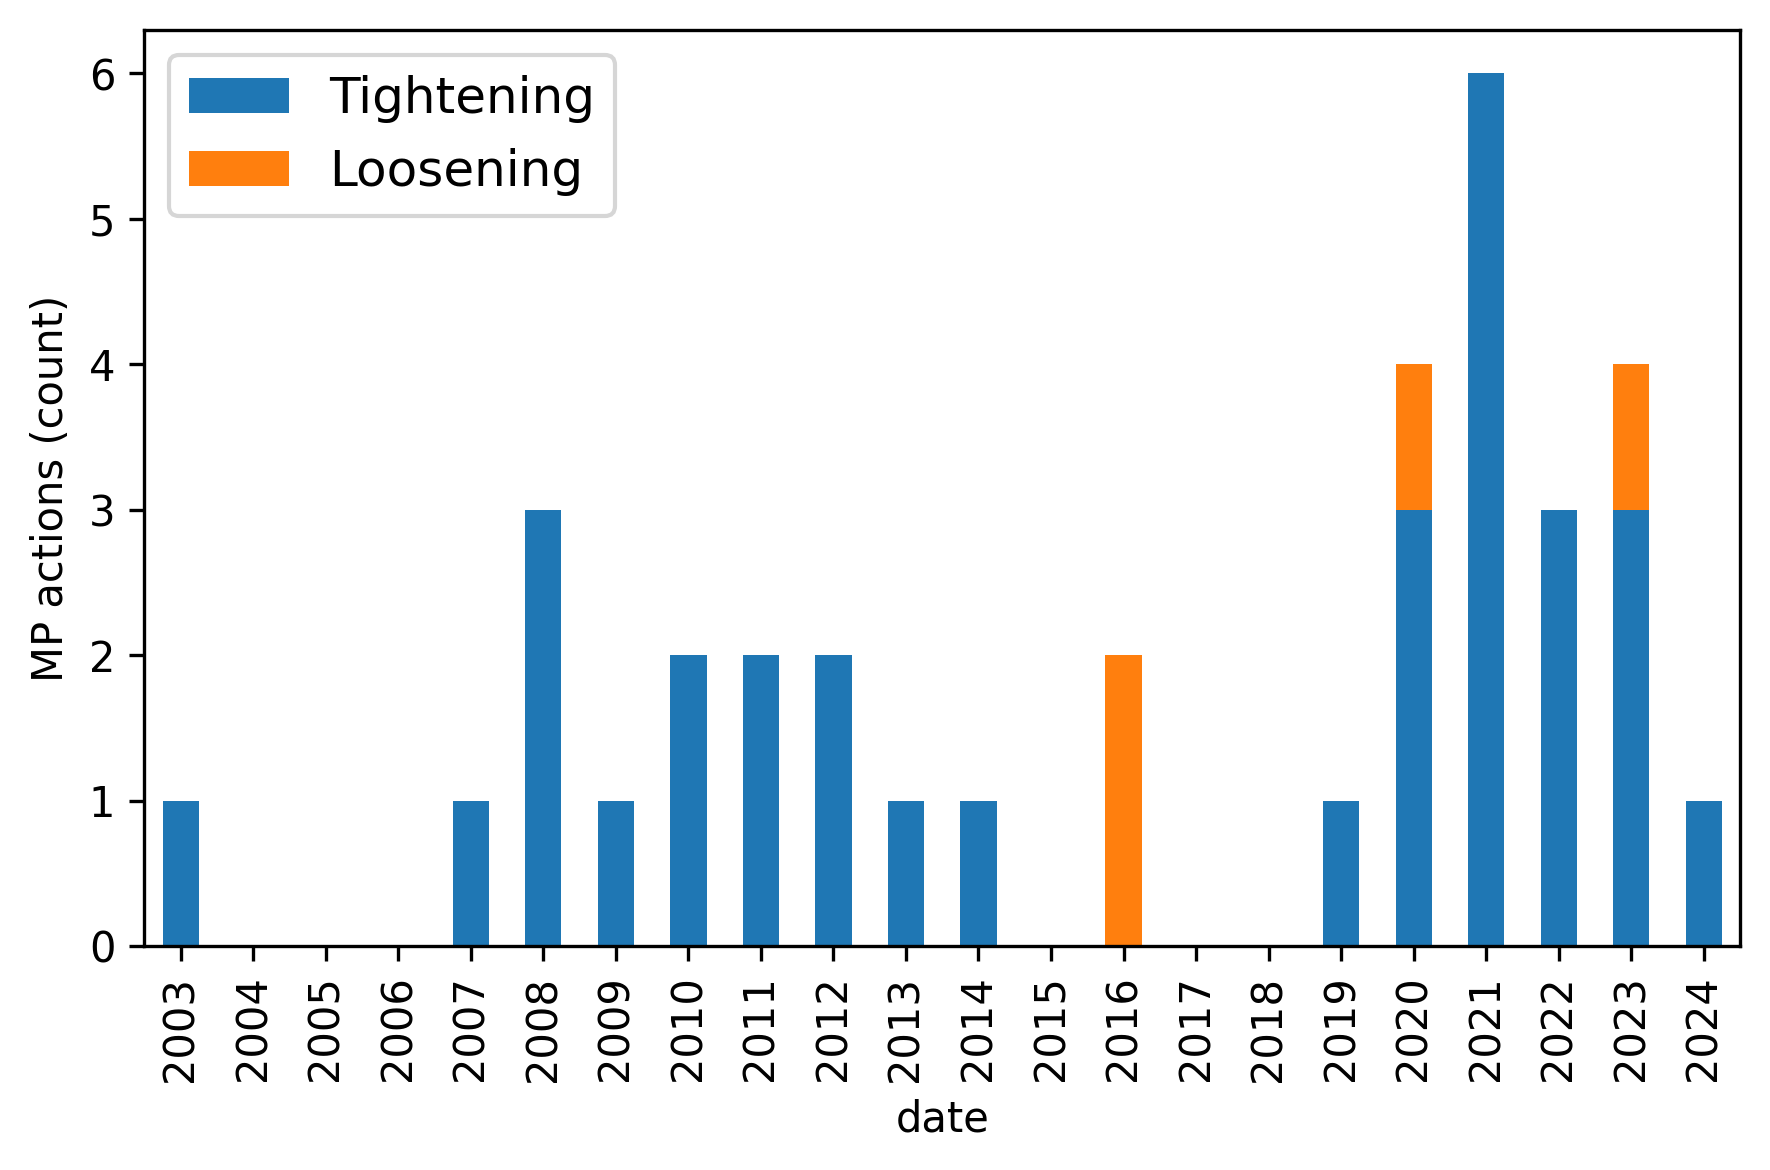
\includegraphics[width=0.9\textwidth, angle=0]{../../../Results/arm_MPI_actions.png}    
    \caption{Use of macroprudential policy in Armenia. The Y-axis shows the number of policy actions taken. in 2014, there has been a very sharp increase in provisioning rates to counter AMD depreciation tendencies, which is counted as a single action here. Large number of tightening actions during and after COVID-19 crisis is due to scheduled rise in Capital conservation buffer and SIFI buffer. } 
    \label{fig:arm_MPI_actions}%
\end{figure}

In 2020, the CBA adopted a more accommodative stance in response to the economic impacts of the Covid-19 pandemic. Specifically, funds received from state support programs were exempted from reserve requirements, providing relief to banks during the economic downturn. Other policy measures included relief of buffer requirements (not loosening the requirement, but usage of the buffers without penalties), etc. This marked a temporary shift toward loosening regulatory requirements to support financial stability during the crisis.

In April 2022, taking into account the pace of risk accumulation in real estate sector, the CBA implemented currency-based loan-to-value (LTV) caps, setting a maximum LTV ratio of 90\% for real estate loans in AMD and 70\% for those in FX. Lastly, during the same year, although the minimum CAR was reduced from 12\% to 11\%, the net stance of macroprudential policy was more restrictive than accomodative, as previously planned increases of other capital-based instruments took place. At year later the CBA indroduced the concenpt of cycle-neutral positive rate of the CCyB, and within following few quarters increased the actual CCyB rate to match the neutral level (it was raised from 1\% (effective from May 2023) to 1.5\% (effective from August 2023)). Simultaneously, the buffer for systemically important financial institutions (SIFIs) increased from 1\% to 1.5\%, and the capital conservation buffer (CCoB) was raised from 1.5\% to 2\%. Collectively, these measures resulted in a net tightening of the macroprudential policy.
\begin{figure}[!ht]
    \centering 
    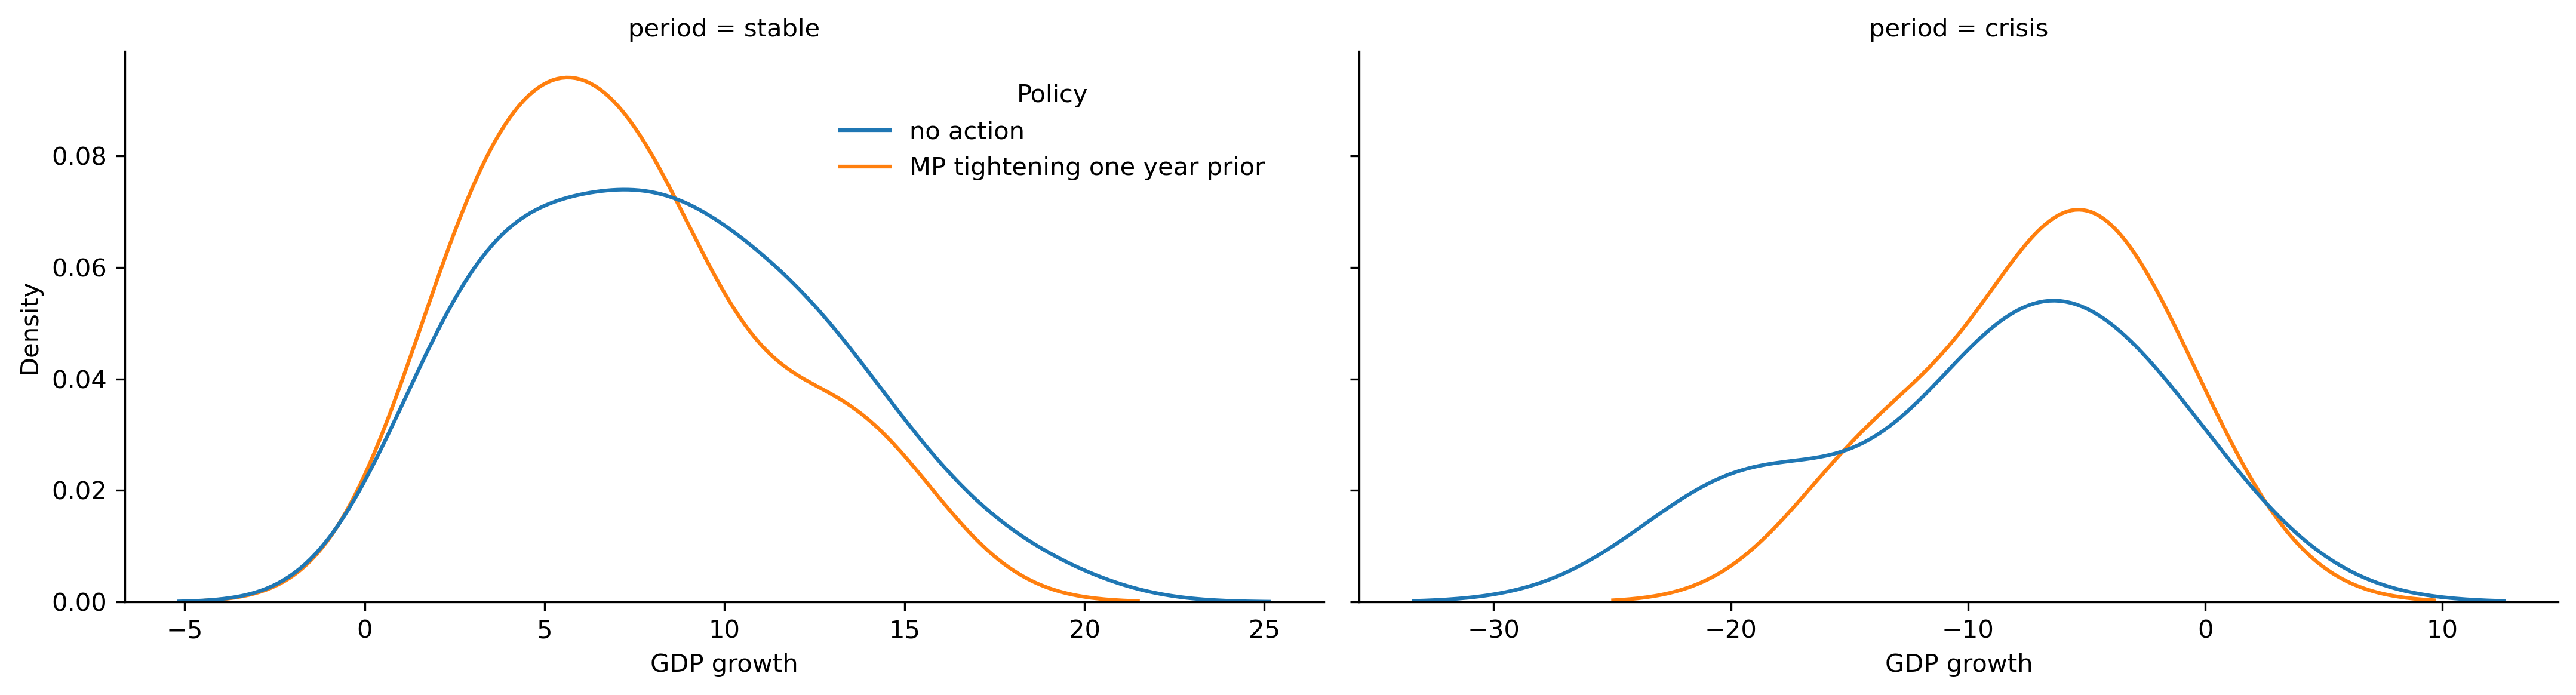
\includegraphics[width=0.9\textwidth, angle=0]{../Figures/arm_MPI_tightening_gdp_dist.png}    
    \caption{Use of macroprudential policy in Armenia (tranquil vs crisis times).} 
    \label{fig:arm_MPI_tightening_gdp_dist}%
\end{figure}

To analyze the impact of these policies we compare the GDP growth distribution of Armenia one year after tightening actions in tanquil vs stress times, as shown in \autoref{fig:arm_MPI_tightening_gdp_dist}. The results indicate that when tightening actions are not followed by a crisis, there is little effect on the left tail of the distribution. However, these actions tend to reduce the right tail, suggesting that they may limit the potential for excessive economic growth. Meanwhile, when a tightening action is followed by a crisis, the distribution shows a less severe left tail. This suggests that tightening policies may mitigate the severity of economic downturns. Finally, the right tail remains relatively unaffected.

To continue our analysis of the evolution of macroprudential policy, in \autoref{fig:panel_MP_use_TL} we investigate the tightening and loosening measures used in the other 40 countries of our study. We observe an active use of loosening measures during the 2008-2009 crisis, in 2012 during the European debt crisis, and during the 2020 Covid-19 pandemic. We also observe an increase in the number of tightening measures starting 2015. \autoref{fig:panel_MP_action_decomp} also delves deeper into the specific measures used over time. In 2009 and 2012 the majority of loosening measures were implemented thought reserve requirements, while in 2020 a much wider array of tools was available for the policymakers, including capital and liquidity-based measures, loan loss provisions (LLPs), LTV measures, and many others \citep{mack2021}. Lastly, the increase in tightening measures in 2015 was primarily driven by the introduction of capital conservation buffers and liquidity measures such as liquidity coverage ratio (LCR), liquid asset ratio (LAR), and net stable funding ratio (NSFR).
\begin{figure}[!ht]
    \centering 
    
\includegraphics[width=0.9\textwidth, angle=0]{../Figures/panel_MP_use_TL.png}    
    \caption{Use of macroprudential policy in 41 countries. The Y-axis shows the number of policy actions taken.} 
    \label{fig:panel_MP_use_TL}%
\end{figure}
\begin{figure*}[!ht]
    \centering 
    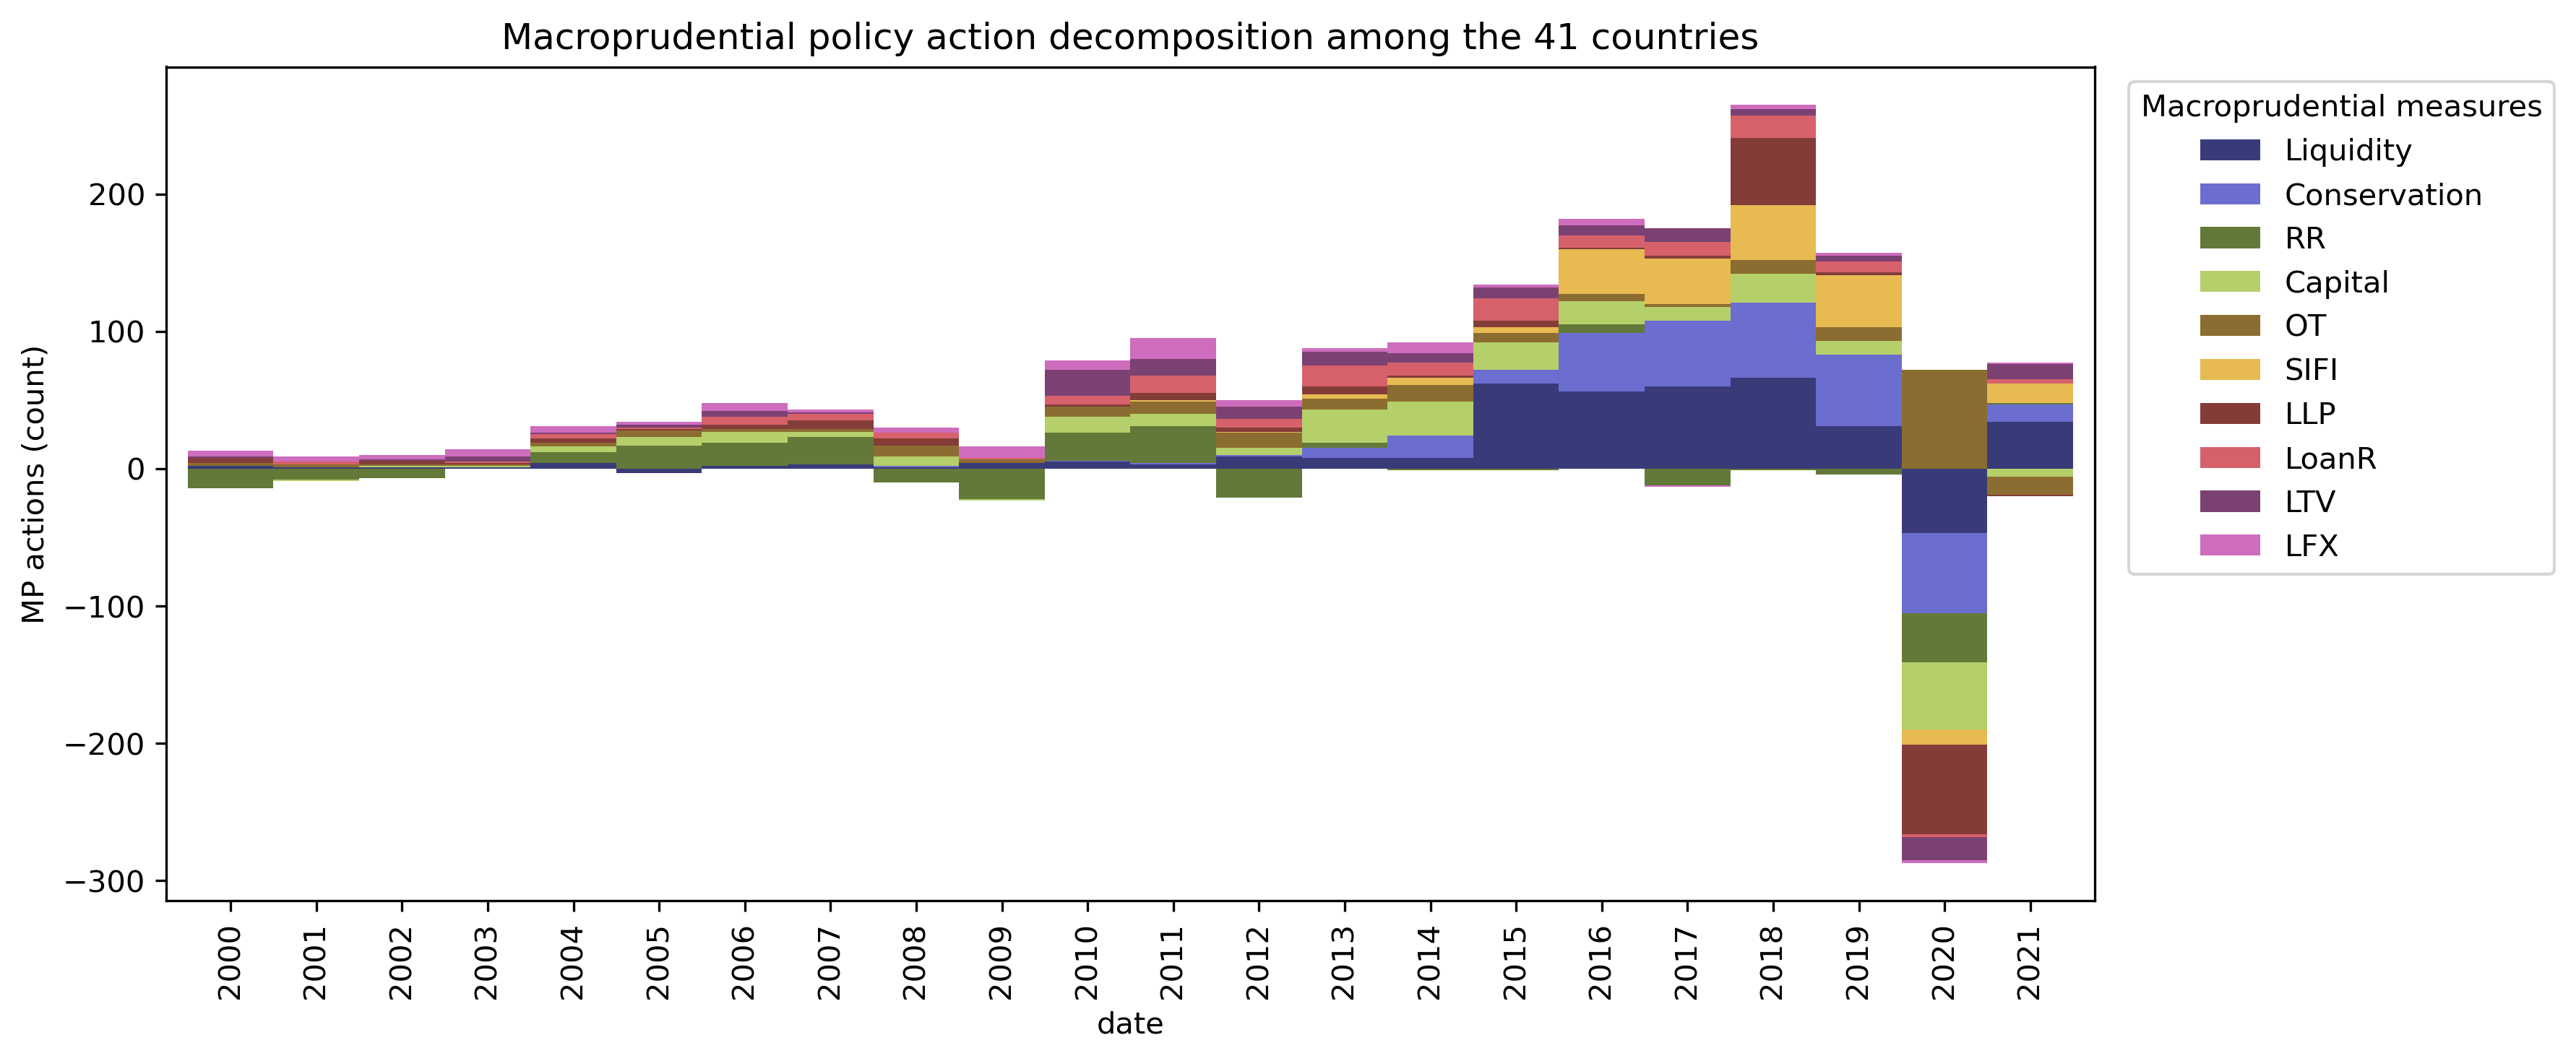
\includegraphics[width=0.9\textwidth, angle=0]{../Figures/panel_MP_action_decomp.png}    
    \caption{Use of macroprudential policy in 41 countries and decomposition of macroprudential measures. The Y-axis shows the net number of tightening vs loosening policy actions taken.} 
    \label{fig:panel_MP_action_decomp}%
\end{figure*}

We examine the impact of macroprudential policy on the GDP growth distribution of the 41 countries in \autoref{fig:panel_MP_use_before_crisis}. During the crisis period the major difference is observed on the right tail of the distribution, which may imply faster recovery \citep{stojkov2020}. The difference becomes more significant when examining the recovery period. Countries that had implemented prior tightening measures had higher GDP growth in this period, and this is broadly consistent with what we have observed in the case of Armenia \autoref{fig:arm_MPI_tightening_gdp_dist}.
\begin{figure*}[!ht]
	\centering 
	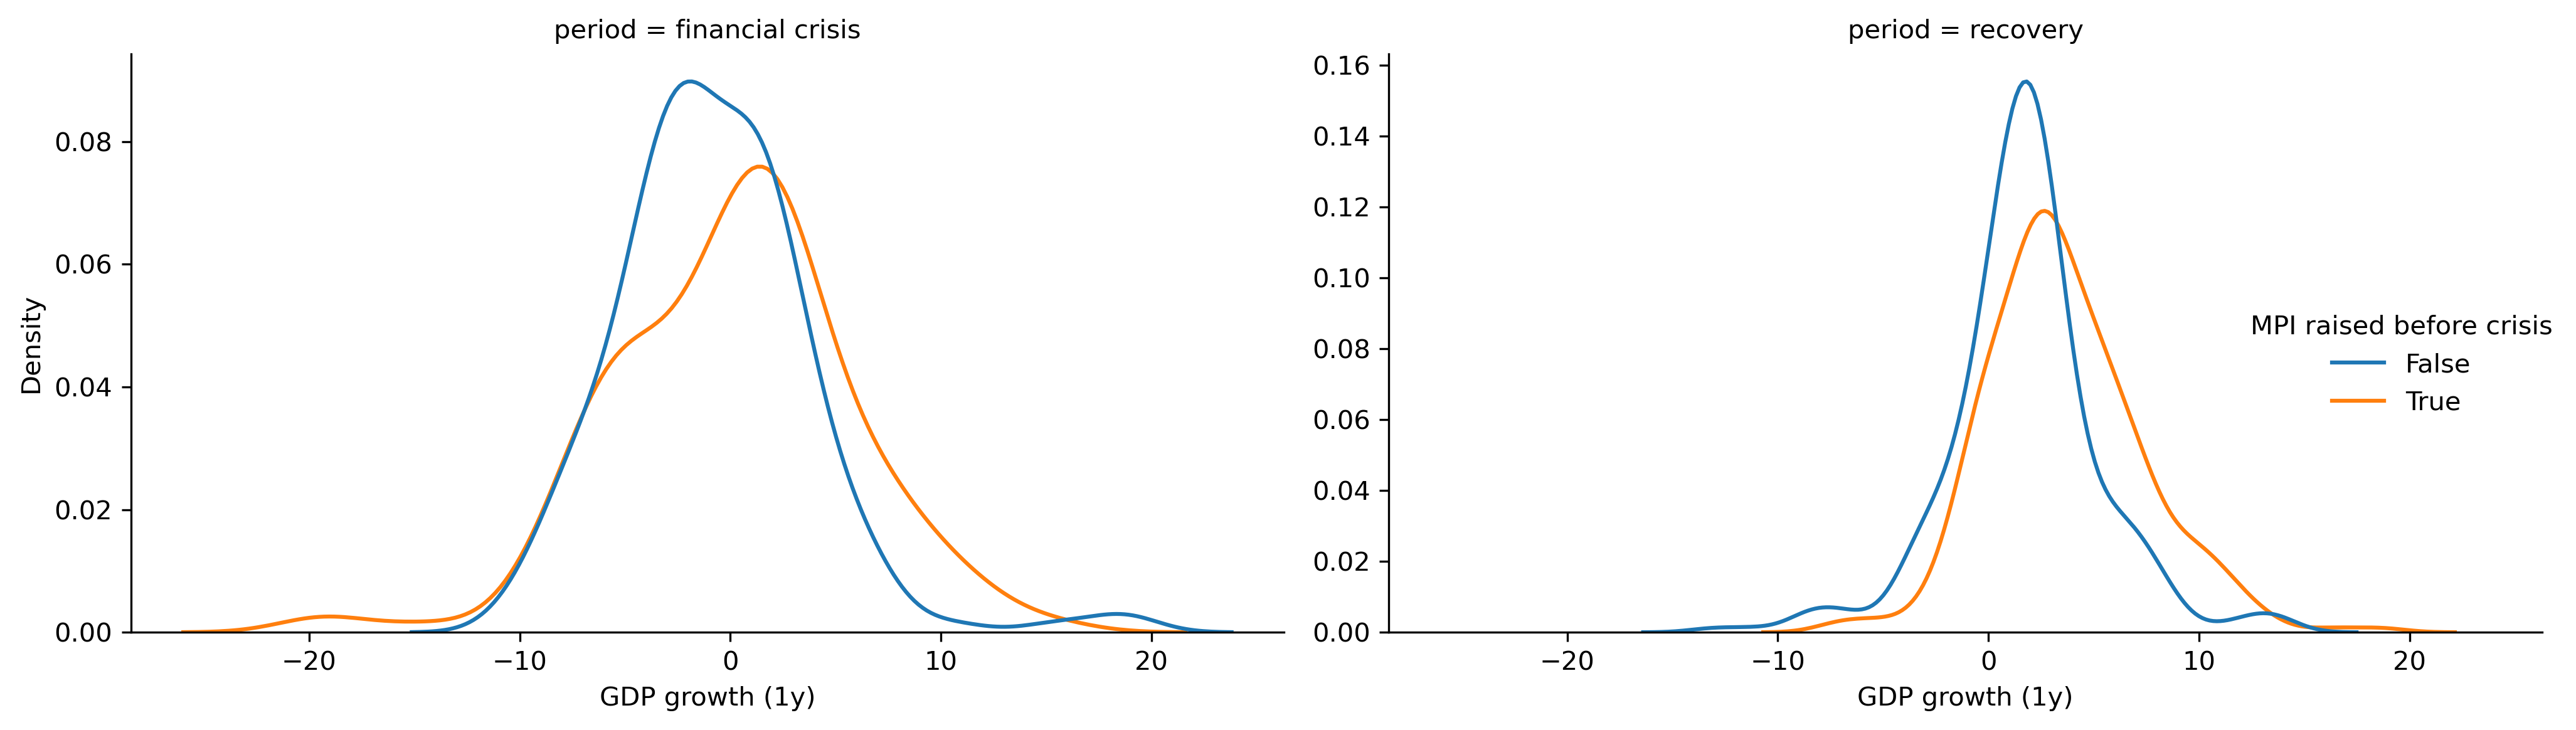
\includegraphics[width=1\textwidth, angle=0]{../Figures/panel_MP_use_before_crisis.png}	
	\caption{GDP growth distribution of 41 countries that implemented macroprudential policy tightening one year before a major crisis.} 
	\label{fig:panel_MP_use_before_crisis}%
\end{figure*}

\subsection{Materialization of risks}
Macroprudential policy affects the GDP growth distribution with two main channels: regulating the buildup of systemic risks (moderating the cycle) and building capital cushions to absorb losses and support normal lending in crisis episodes. These systemic risks tend to accumulate during periods characterized by rising asset prices and low market volatility. In such environments, the ease of borrowing encourages economic agents to increase leverage. From the supply side these conditions reduce the incentives of financial intermediaries to wisely manage liquidity and solvency risks due to rising risk appetite. This leads to negative externalities, manifesting as ``increased leverage, mismatches of maturity and financial positions, growing indebtedness, reduced debt servicing capacity, and other balance sheet weaknesses'' \citep{imf_gar_2019}. Consequently, during periods of financial stress, banks tend to reduce lending and engage in deleveraging, which further exacerbates the decline in asset prices. Ultimately, these exposures contribute to deeper, more prolonged, and severe economic downturns \citep{Cardarelli_2011}.

In \autoref{fig:theory_gdp_unconditional}, we present the unconditional GDP growth distribution of Armenia. The dotted lines represent the median and the 10th percentile (or tail) of the distribution. The difference between the median and the tail, referred to as the ``distance-to-tail'', reflects the unconditional risks faced by the financial system. This metric captures not only the direct impact of potential crises but also the amplifying effects of systemic risks. In the case of Armenia, a crisis, defined as the worst 10\% of possible outcomes, could reduce GDP growth by up to 12.4\%.
\begin{figure}[!ht]
    \centering 
    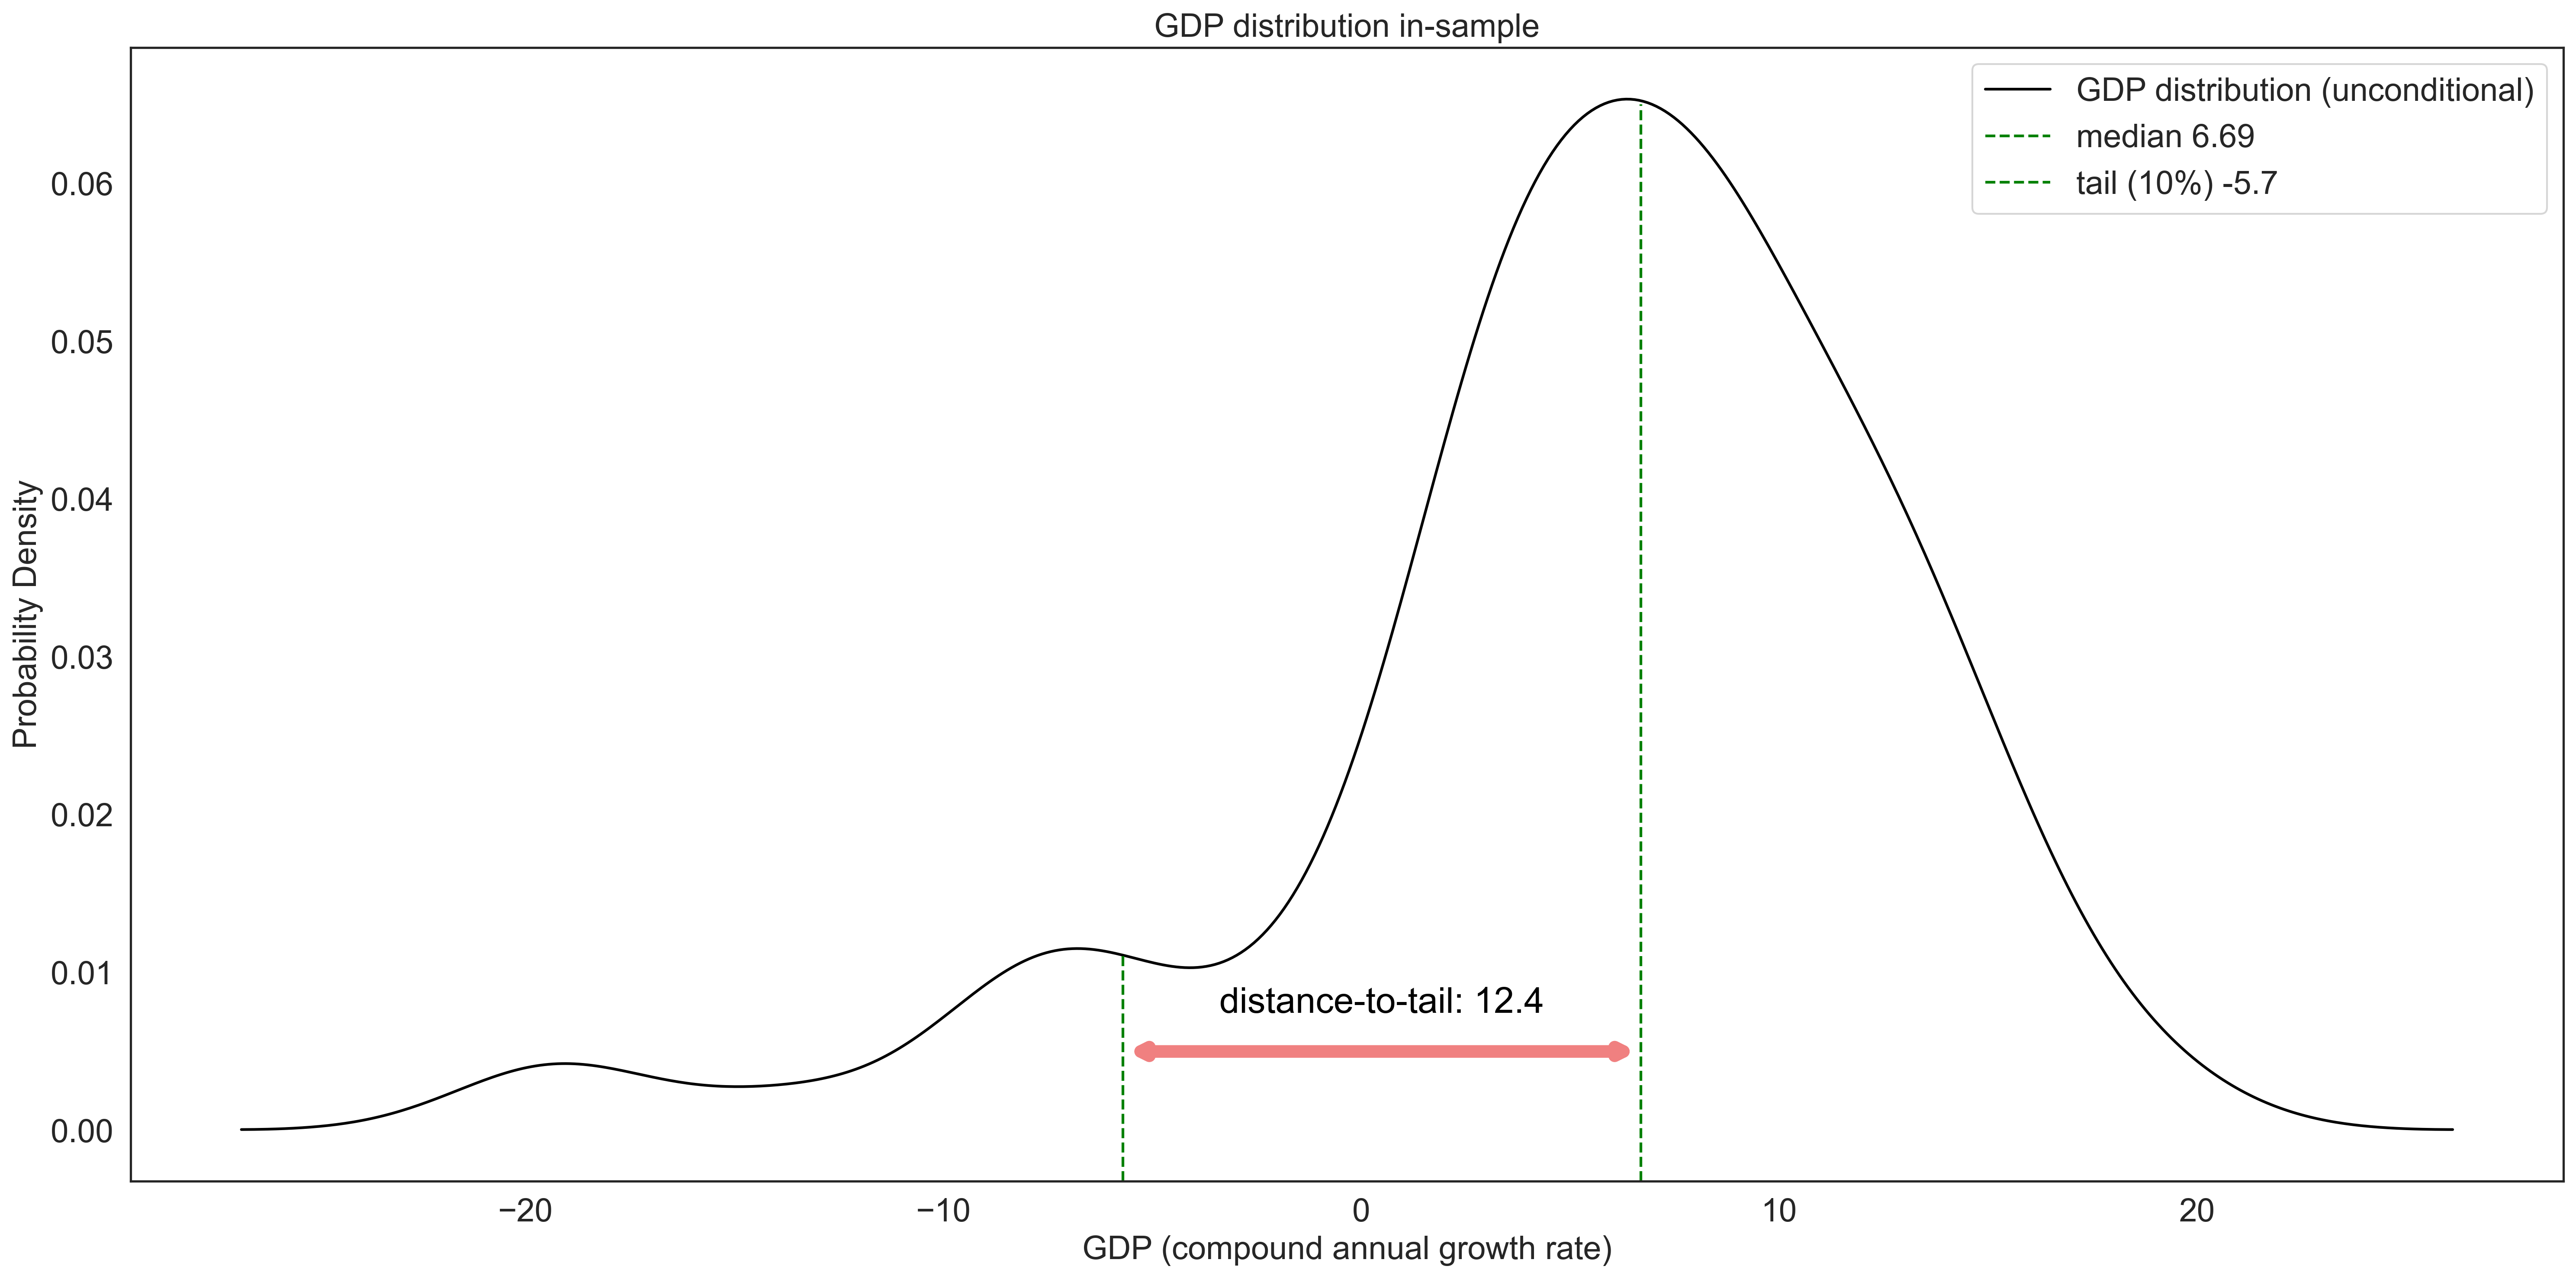
\includegraphics[width=0.9\textwidth, angle=0]{../Figures/theory_gdp_unconditional.png}   
    \caption{Unconditional GDP growth distribution of Armenia and distance-to-tail.} 
    \label{fig:theory_gdp_unconditional}%
\end{figure}

In \autoref{fig:theory_policy}, we illustrate the GDP growth distribution of Armenia conditional on systemic risks. This conditional distribution displays how the risks shape the uncertainty surrounding GDP growth expectations. The conditional distance-to-tail serves as a means to quantify the negative impact that the buildup of systemic risks can exert on the economy. In the same figure, we simulate how a buildup of financial vulnerabilities, such as excessive credit growth a year prior will affect the shape of the distribution (shown in yellow). This type of environment may increase or decrease the median depending on the nature of externalities, but it will always negatively affect the tail. The distance-to-tail will sharply increase as a result, reflecting the potential severity of these risks. Lastly, we simulate the impact that a tightening of the macroprudential policy during excessive credit growth might have on the distribution (shown in green). While tightening policies tend to lower the median due to the short-term costs imposed on banks, they also improve the tail outcomes. As a result, the distance-to-tail decreases, signaling a reduction in negative outcomes related to systemic risks. This is both a result of the reduction in risks, but also the increased resilience of the system.
\begin{figure}[!ht]
    \centering 
    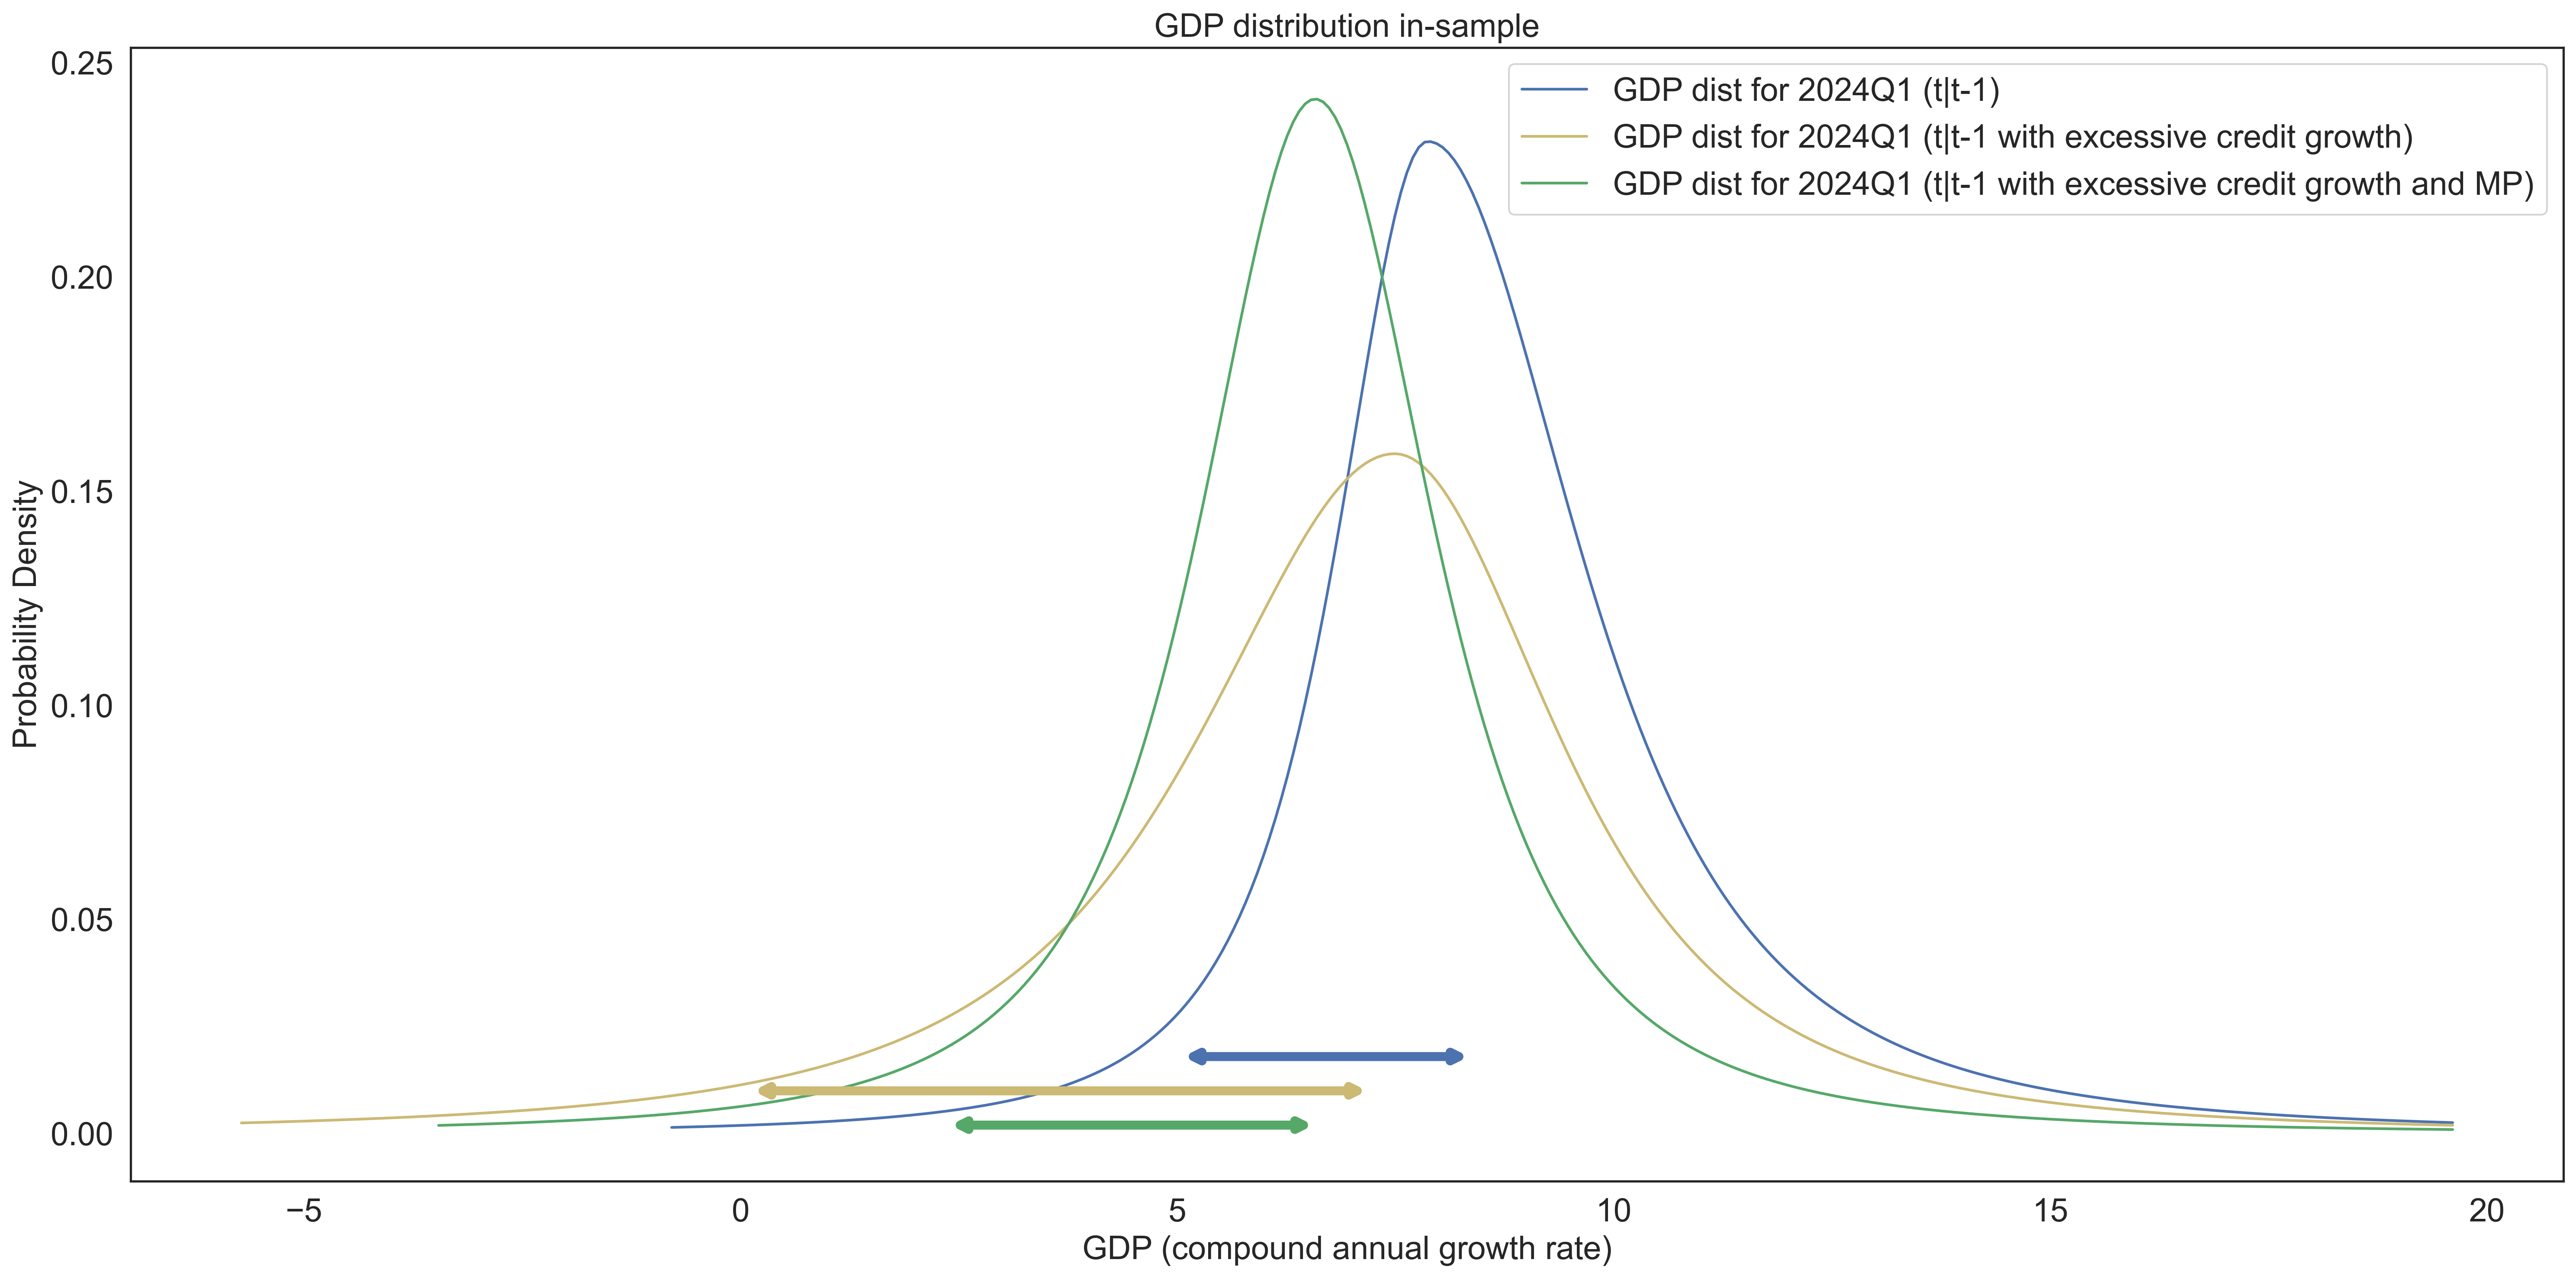
\includegraphics[width=0.9\textwidth, angle=0]{../Figures/theory_policy.png}  
    \caption{GDP growth distribution of Armenia conditional on systemic risks in 2024Q1. The yellow distribution considers the effect of an increase in financial vulnerabilities, while the green distribution considers the former, but also a tightening of macroprudential policy.} 
    \label{fig:theory_policy}%
\end{figure}


\section{Methodology}
\subsection{Panel quantile regression}
As we have discussed before, macroprudential policy has different effects on the median and tails of GDP growth distribution \citep{boar_2017}. To model these nonlinearities we use the quantile regression framework \citep{koenker_1978_regression} which allows us to focus on different conditional quantiles of the distribution and not just the conditional mean. Quantile regression has also become quite popular in forecasting growth-at-risk, which is the term indicating the expected loss in GDP growth given a tail event. Put another way, it is a measure of how big will the loss of GDP be, given that adverse shock happens. In fact, it has proven to outperform GARCH-type models \citep{kipriyanov_2022} in this task. In a panel framework, quantile regression helps to account for heterogeneous covariates, while the fixed effects consider the unobserved heterogeneity which does not change with respect to time \citep{galan2020}. It is important to note that in this framework the fixed effects are subject to change depending on the quantile. For a general case, a panel quantile regression takes the following form:
\begin{equation}
    \label{eq:panel_qr}
    y_{i,t+h} = \alpha_{i, \tau} + X_{i,t} \beta_\tau + \nu_{\tau,t+1}
\end{equation}
\begin{equation}
    \label{eq:panel_qr_loss}
    \nu_{\tau,t+1} = \sum_{i=1}^n \sum_{t=1}^{T-h}\rho_\tau| y_{i,t+h} -  y_{i,t+h}^*|
\end{equation}
\begin{equation}
    \label{eq:panel_qr_weights}
    \rho_\tau = \tau \cdot 1_{y_{i,t+h} \geq y_{i,t+h}^*} + (1-\tau) \cdot 1_{y_{i,t+h} < y_{i,t+h}^*}
\end{equation}

where, $y_{i,t+h}^*$ is the quantile regression estimate, $X_{i,t}$ is a vector of exogenous variables, $\alpha_{i, \tau}$ is a vector of fixed effects, $\rho_\tau$ are the quantile-based weights, $\tau\in\Gamma$ is the quantile, while $t\in T$ and $i\in n$ are the time dimension and the cross-section dimension respectively. In our case $T$=120 and $n$=41. An important note is that the model uses least absolute deviation (LAD) as its optimality criterion.

\subsection{Quantile regression for Armenia (local model)}
The baseline quantile regression model for the Armenian economy takes the form:
\begin{equation}
    \label{eq:local_qr}
    \begin{aligned}
    y_{t+h} = 
    &\;\alpha_\tau + \beta_{1, \tau}y_t + \beta_{2, \tau}\text{FCyI}_t + \beta_{3, \tau}\text{FCI}_t + \beta_{4, \tau}\text{CI}_t \\
    &+ \beta_{5, \tau}\text{MPI}_t + \beta_{6, \tau}\text{CAR}_t + \beta_{7, \tau}\text{LR}_t + \beta_{8, \tau}\text{MI}_t \\
    &+ \beta_{9, \tau}\text{CyBPA}_t + \beta_{10, \tau}\text{CBPA}_t + \varepsilon_{t, \tau}
    \end{aligned}
\end{equation}

In this specification $y_{t+h}$ is the annualized average growth rate of real GDP at $t+h$ quarters ahead. The $\alpha_\tau$ is an intercept, $y_t$ is the autoregressive component, $\text{FCyI}_t$ is the financial cycle index, $\text{FCI}_t$ is the financial conditions index, and $\text{CI}_t = St(\text{FCyI}_t) \cdot St(\text{FCI}_t)$ is the ``crisis index'', which is the product between the standardized $\mathcal{N}(0, 1)$ $\text{FCyI}_t$ and $\text{FCI}_t$.

Next, we include the macroprudential policy index $\text{MPI}_t$, the 2-year change in the excess capital adequacy ratio (actual CAR level minus minimum requirement) $\text{CAR}_t$, and the excess liquidity ratio (HQLA/Assets) $\text{LR}_t$.
The rest of the model includes a control variable, the macroeconomic indicator $\text{MI}_t$, which as was mentioned above, has two roles: capturing the risks originated not from financial system, but from broader macroeconomy, and serving as a control variable.

Finally, we include the interaction terms with the MPI, specifically, the Cycle-Based Policy Adjustment $\text{CyBPA}_t$ and the Conditions-Based Policy Adjustment $\text{CBPA}_t$, which were discussed in the previous section.


\subsection{Parametric fit}
After evaluating the quantile regression models, we end up with conditional quantile estimates $y_{t+h, \tau}^*$. With a sufficiently large set of quantiles $\Gamma$, one can describe the conditional cumulative distribution function (CDF) of the output growth at time $t+h$. To derive the probability distribution function (PDF) a parametric t-skew fit \citep{adrian_2019} is used. Compared to the normal distribution, the t-distribution is much better suited for capturing the fat tails. Using the closed-form specification of the distribution proposed by \citet{giot2003} we define the CDF as:
\begin{equation}
    \label{eq:tskew_cdf_n}
    F(x, \mu, \sigma, \text{df}, \xi) = \frac{2}{1+\xi^2} T_{cdf}\left(\frac{x-\mu}{\sigma}\xi, \text{df}\right), \;\text{if}\; x \leq \mu 
\end{equation}
\begin{equation}
    \label{eq:tskew_cdf_p}
    F(x, \mu, \sigma, \text{df}, \xi) = 1 - \frac{2}{1+\frac{1}{\xi^2}} T_{cdf}\left(-\frac{x-\mu}{\sigma}\frac{1}{\xi}, \text{df}\right), \;\text{if}\; x > \mu 
\end{equation}

where $\mu$ and $\sigma$ are the location and scale parameters, while $\xi$ is the skewness. To simplify the search space to only three parameters we anchor the degrees of freedom at 2 ($\text{df}=2$). Finally, we define the optimization function in terms of quantiles:
\begin{equation}
    \label{eq:tskew_cdf_loss}
    \mu_{t+h}^*, \sigma_{t+h}^*, \xi_{t+h}^* = arg\,min\left(\sum_\tau \left(F(y_{t+h, \tau}^*, \mu, \sigma, \text{df}^*, \xi)-\tau\right)^2\right)
\end{equation}

After the location, scale, and skewness parameters are estimated they can be used to generate the t-skew PDF and CDF at time at time $t+h$.

\subsection{Macroprudential stance}
Generally, when considering macroprudential policy through the ``risk-resilience framework'', a stance metric represents the residual systemic risk in the financial system \citep{esrb2019}. We derive the residual risk by ``assessing the aggregate risk and subtracting any exogenous and/or policy-induced resilience'' \citep{esrb2021}. From this perspective, macroprudential policy is a risk management approach, where we balance systemic risk and resilience while accounting for policymakers' tolerance of the net residual risk. As part of the indicator-based approach for Borrower-Based Measures (BBMs), \citet{esrb2024} defines the macroprudential stance as:
\begin{equation}
    \label{eq:stance}
    \textnormal{Stance} = \textnormal{Risk} - \textnormal{Resilience} - \textnormal{Policy}
\end{equation}

In the GaR framework, the conditional distance-to-tail tracks the changes in systemic risk over time, thus it can be used as one of the main indicators for the macroprudential stance. The metric primarily focuses on risks and policy, while using systemic thresholds as a reference for resilience. The systemic thresholds are calculated from the quantiles of the historical distance-to-tail series. The loss function for the distance-to-tail approach takes the form:
\begin{equation}
    \label{eq:dt_loss}
    \min_{\rho_t}\mathcal{L} = \max{\left((y_m - y_c), \textnormal{threshold}\right)}
\end{equation}

where $y_m$ and $y_c$ are the median and the tail, while ($y_m-y_c$) is the distance-to-tail. When this value exceeds the threshold, we are incentivized to tighten the macroprudential policy to minimize the loss. The complete \citet{esrb2024} formulation includes multiple thresholds at the 10th, 30th, 70th, and 90th percentiles of the distance-to-tail distribution. The resulting stances are classified into 5 categories: tight, grey-tight, neutral, grey-loose, and loose. Thus, the long-term goal of the policy is to maintain the stance at the neutral level.

The main limitation of this approach is that it does not consider the costs that macroprudential policy will impose for reducing systemic risks, put another way - it just shows the direction of macroprudential policy, not the size of action nor the costs associated with it. Additionally, the systemic thresholds are not a dynamic measure of the resilience of the financial system. 

As an alternative to the distance-to-tail approach, we consider the welfare function proposed by \citet{suarez2022}. The function takes the form:
\begin{equation}
    \label{eq:suarez_W}
    W = y_m - \frac{1}{2}w\left(y_m - y_c\right)^2
\end{equation}
\begin{equation}
    \label{eq:suarez_loss}
    \min_{\rho_t}\mathcal{L} = -\mathop{\mathbb{E}_t}\left\{\sum_{t=0}^{T}\beta^tW_{t+1}\right\}
\end{equation}

where $w$ is interpreted as the aversion to financial instability, while $\beta$ is a discount factor. This formulation considers both the median and the distance-to-tail, capturing the costs of macroprudential policy along with its benefits \citep{cecchetti_2021}. It is apparent from \autoref{eq:suarez_W}, that the optimal policy is subject to the choice of $w\in(0,\inf)$. This term includes the policymakers' appetite for risk, but also the probability of crisis. A higher value of w indicates that the policymaker is more sensitive to risks, while a value of zero would imply a complete disregard for the systemic risks in the economy. The calibration results indicate that the reasonable value of $w$ in Armenia is around 0.11\footnote{For detailed information on the calibration procedure, see \ref{appx:w_calibration}.}. The specific trade-off for the policymakers will depend on their tolerance for downside risks, but also the effectiveness of macroprudential policy \citep{esrb2021, suarez2022} \footnote{For details, please see \ref{appx:suarez}.}.

\subsection{Addressing Endogeneity}

As in many papers in the topic, the model in this paper faces the challenge of policy endogeneity. In other words, the expectations of economic growth may influence policy decisions, thus creating reverse causality that distorts our inference. This endogeneity adds bias to the coefficients that we estimate. The true effect of an exogenous change might be different from what was observed. Given that indicators such as the Credit to GDP gap have historically influenced macroprudential policy decisions, addressing this bias is essential. Additionally, closed-form regressions can not capture the nonlinear interactions between macroprudential policy and systemic risks, also exposing other coefficients to the endogeneity issue.
In the paper, we address the issue of endogeneity using three complementary strategies.
\begin{enumerate}
    \item First, we treat MPI (Macroprudential policy index) by estimating non-systemic policy shocks by regressing MPI on systemic risks and then extracting the residual (the constant is added back in). This essentially acts as the subset of macroprudential policy decisions not driven by prevailing economic conditions. It ensures that MPI is uncorrelated with systemic risks.
    \item Second, in the MCMC specification of the model, we estimate the coefficient of MPI as a nonlinear function of systemic risks. Thus, instead of looking at the subset of cases, this approach attempts to eliminate the bias by more closely modeling the relationship between policy decisions and risks. 
    \item Finally, for both approaches above, we use priors derived from the more robust panel specification of the model. This mitigates the coefficient instability (offshoots) caused by endogeneity, under the assumption that country-specific biases are random, yet consistent across time, and follow a white noise process.
\end{enumerate}




\section{Results}
\subsection{Quantile regression estimates for panel and local models}
To analyze the relationship between systemic risks, macroprudential policy, and GDP growth, we use the model estimates of \autoref{eq:panel_qr} and \autoref{eq:local_qr} as the foundation for the comparisons. \autoref{fig:arm_qr_f_r2} and \autoref{fig:panel_r2} illustrate the goodness of fit of the local and panel quantile regression models respectively across various quantiles and horizons. Specifically, horizons 4, 8, and 12 represent GDP growth projections for 1, 2, and 3 years ahead. The models demonstrate optimal in-sample performance at the lower and upper quantiles of the GDP growth distribution. This outcome is by design since our focus is on tail risks. In the panel model, the strongest fit occurs when predicting GDP growth 2-3 years ahead, whereas the local model excels in forecasting 1-2 years ahead. This may suggest that the lag between systemic risk buildup and its materialization is shorter in Armenia compared to other countries. Therefore, we adopt the 1-year ahead estimates as the primary benchmark for our comparisons and discussions.
\begin{figure*}[!ht]
    \centering 
    
\includegraphics[width=1\textwidth, angle=0]{../Figures/arm_qr_f_r2.png}   
    \caption{Pseudo r-squared for local quantile regression estimates across quantiles and horizons. OLS r-squared is displayed as a dashed line. Note: generally, quantile regression and OLS (pseudo) r-squared are not comparable. They are here for convenience.}
    \label{fig:arm_qr_f_r2}%
\end{figure*}
\begin{figure*}[!ht]
    \centering 
    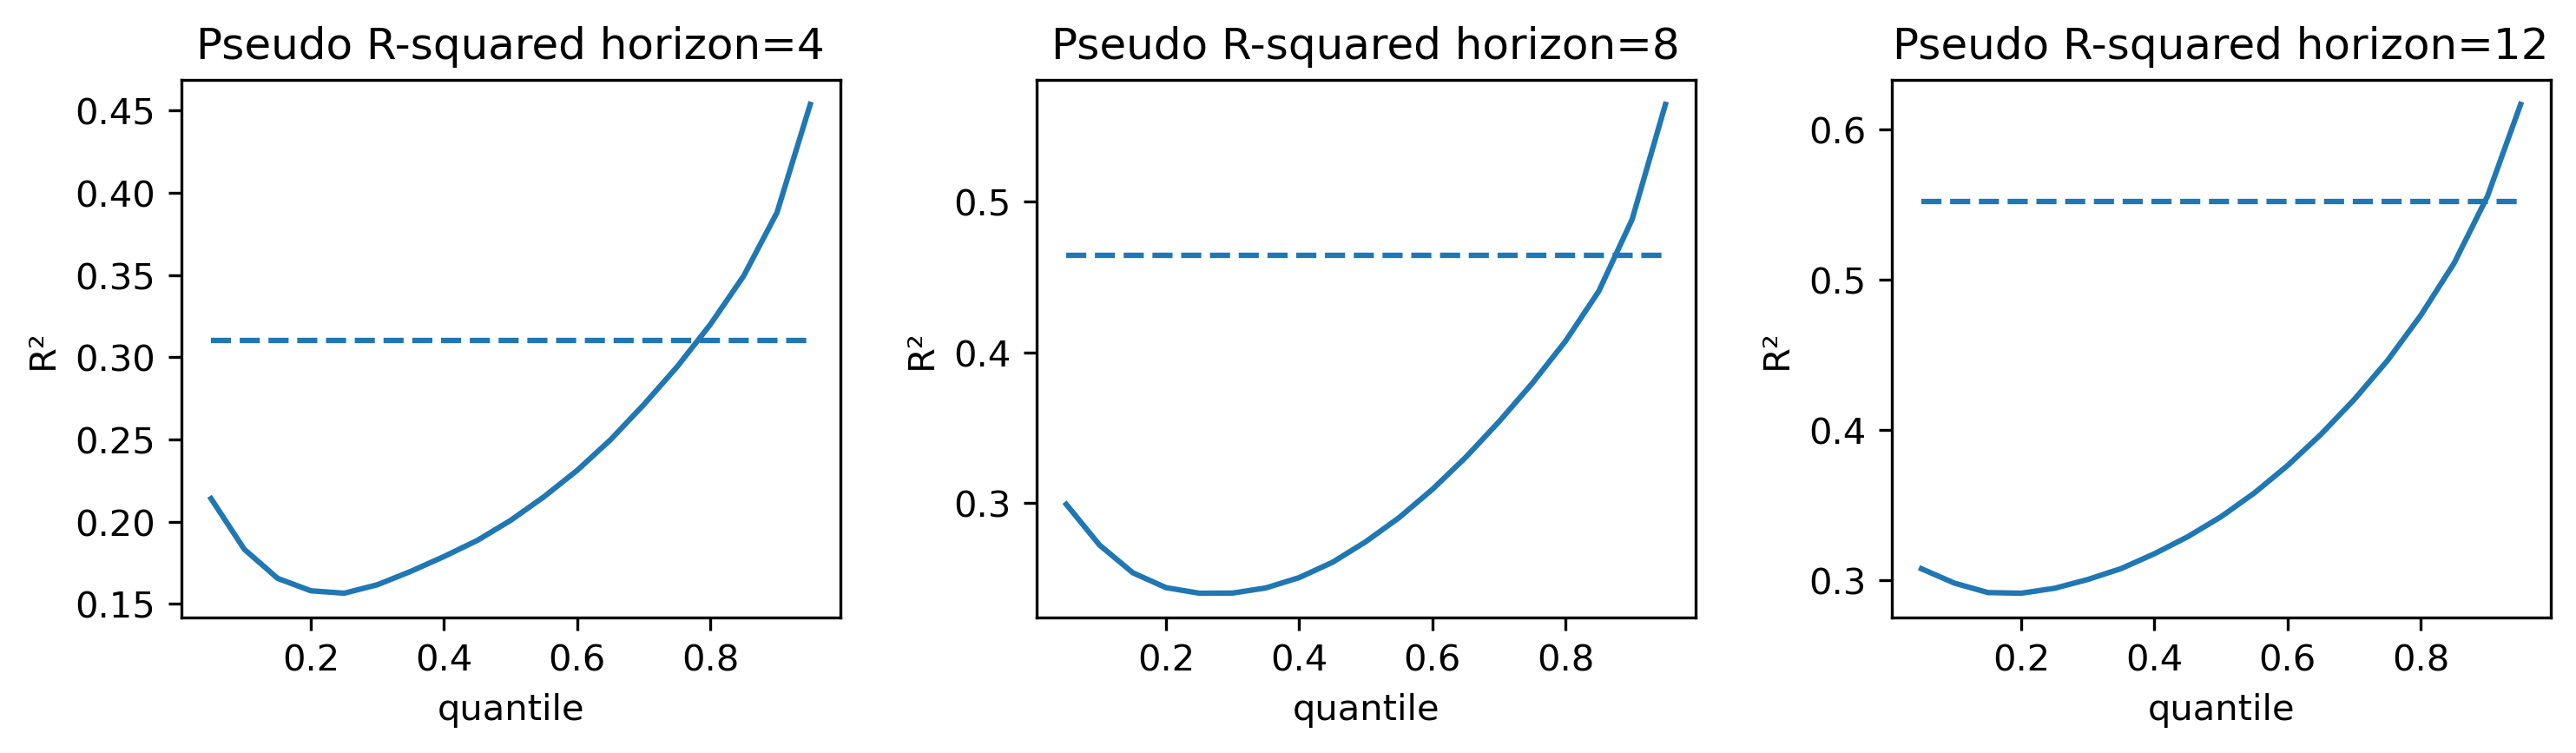
\includegraphics[width=1\textwidth, angle=0]{../Figures/panel_r2.png}  
    \caption{Pseudo r-squared for panel quantile regression estimates across quantiles and horizons. OLS r-squared is displayed as a dashed line.} 
    \label{fig:panel_r2}%
\end{figure*}


\autoref{fig:arm_FCyI_f_coeff_quantiles} and \autoref{fig:panel_FCyI_coeff_quantiles} in \autoref{appx:additional_figures} display the quantile regression coefficients for the FCyI in the local and panel models, respectively. In the local model, the FCyI shows a negative but insignificant effect in the short run, while its negative impact becomes significant over the long run. Conversely, the panel model demonstrates a consistently negative and significant FCyI effect in both the short and long run.

Additionally, the results reveal heterogeneous effects of FCyI across the distribution, with more pronounced impacts in the lower quantiles. This indicates that increases in FCyI exacerbate tail risks, suggesting that it would increase distance-to-tail, which is in line with the theory of business and financial cycles where a maturity or a peak phase is followed by a contraction. The results suggest that financial vulnerabilities affect the economy in the medium term. This relationship was also observed in Portugal where credit aggregates were the most relevant medium term predictors of future GDP growth \citep{imf_gar_2019}.

\autoref{fig:arm_FCI_f_coeff_quantiles} and \autoref{fig:panel_FCI_coeff_quantiles} in the same annex present the quantile regression coefficients for the FCI in both the local and panel models. In the local model, the FCI is positive and largely significant in the short run but becomes insignificant over the long-term. In contrast, the panel model shows that FCI remains significant across both time dimensions, though its effect varies considerably. The FCI negatively impacts the left and right tails while positively influencing the middle quantiles.



A high FCI reflects tight financial conditions. In the near term, this effect should be negative, yet due to its cyclical and mean-reverting nature, it will eventually normalize, boosting future growth \citep{imf_gar_2019}. The positive short-term coefficient in the local model likely reflects this cycle, where financial stress is followed by economic recovery. Meanwhile, the negative effect on the left tail in the panel model underscores the long-term negative externalities that financial stress can create. Overall, the literature suggests that FCI should primarily exert short-term effects on the GDP growth distribution \citep{esrb2021}.

\subsection{The impact of macroprudential policy on output growth distribution}
Macroprudential policy enters the panel and local equations through both direct and indirect (interaction) effects. Direct effects capture the benefits of increased resilience from policy interventions, as well as the associated costs. Interaction effects, on the other hand, capture the role of macroprudential policy in mitigating systemic risks in various situations and times (e.g. when cycle is up or down, or when stress level is elevated or low).

\autoref{fig:arm_MPI_f_coeff_quantiles} and \autoref{fig:panel_MPI_coeff_quantiles} plot the quantile regression coefficients for the direct effects of MPI in the local and panel models, respectively. In the local model, the short-run direct effects are positive at the left tail and negative at the median, though these coefficients are statistically insignificant. The panel model shows similar short-run patterns but with significant effects. Lastly, the long-run direct effects are negative and significant.

\begin{figure*}[!ht]
	\centering 
	
\includegraphics[width=1\textwidth, angle=0]{../Figures/arm_MPI_f_coeff_quantiles.png}	
	\caption{Local model direct Macroprudential Policy Index coefficients. Estimated quantile regression coefficients for horizons 4, 8, and 12. The grey-shaded areas represent the 95\% confidence intervals. The dashed horizontal line presents the OLS coefficient.}
	\label{fig:arm_MPI_f_coeff_quantiles}%
\end{figure*}
\begin{figure*}[!ht]
	\centering
	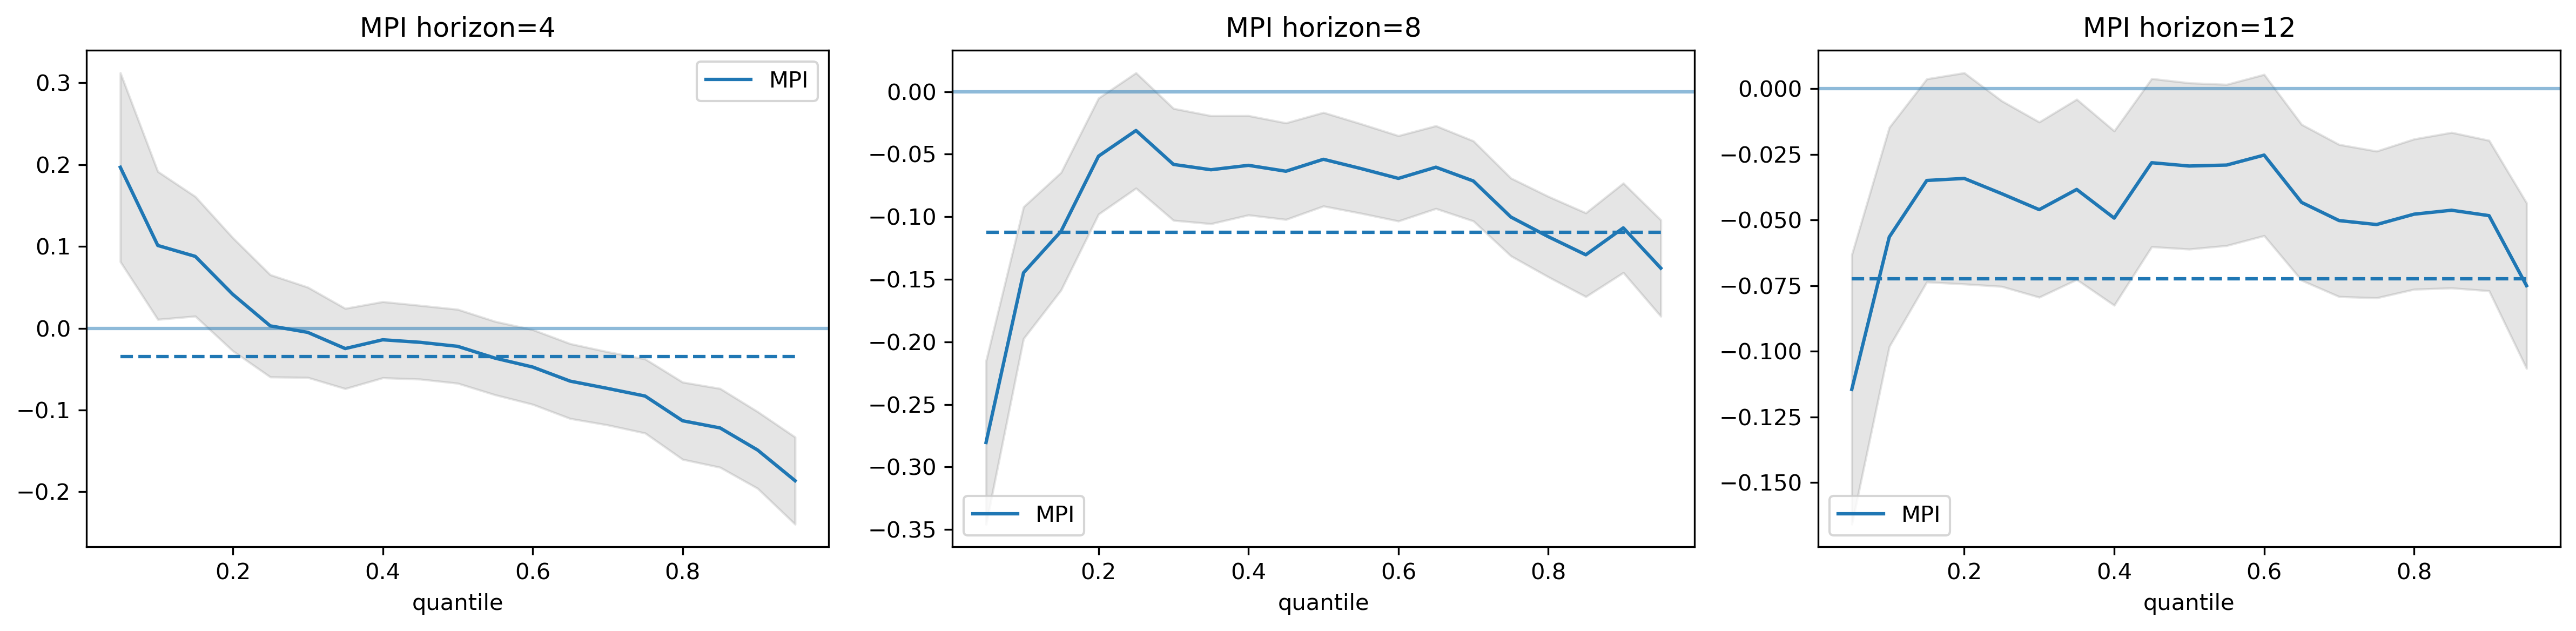
\includegraphics[width=1\textwidth, angle=0]{../Figures/panel_MPI_coeff_quantiles.png}	
	\caption{Panel model direct Macroprudential Policy Index coefficients.} 
	\label{fig:panel_MPI_coeff_quantiles}%
\end{figure*}


The heterogeneity in the direct effects suggests that, in the short run, MPI improves resilience and reduces distance-to-tail. However, if financial conditions remain stable and no crisis is observed, MPI could have negative long-term implications for both the median and distance-to-tail. These outcomes reflect the practical costs of macroprudential policy \citep{schmitz2022eu}, but also the prolonged requirement for banks to hold excess capital, which may suppress economic activity over time.

To examine the overall impact of macroprudential policy, we present the conditional MPI coefficients in \autoref{fig:arm_MPI_cond_coeff_quantiles}. The reason behind this definition is the convention, that the effectiveness and magnitude of performed policy actions will be heavily dependent on the conditions present in the system: whether it is early stage of financial cycle and risks are largely in neutral level or below it, or the system is operating at the peak of financial cycle, where significant amount of risks are accumulated. The situation is further complemented by the level of stress in the system. This has been done by defining a special function, which takes the baseline estimation from the model and transforms it according to the priors we provide for both FCyI and FCI (basically these priors are presented in the figure with numbers: -3 stands for underperformance, 0 for neutral level and 3 for overheating or elevated level of risks).
\begin{figure*}[!ht]
    \centering
    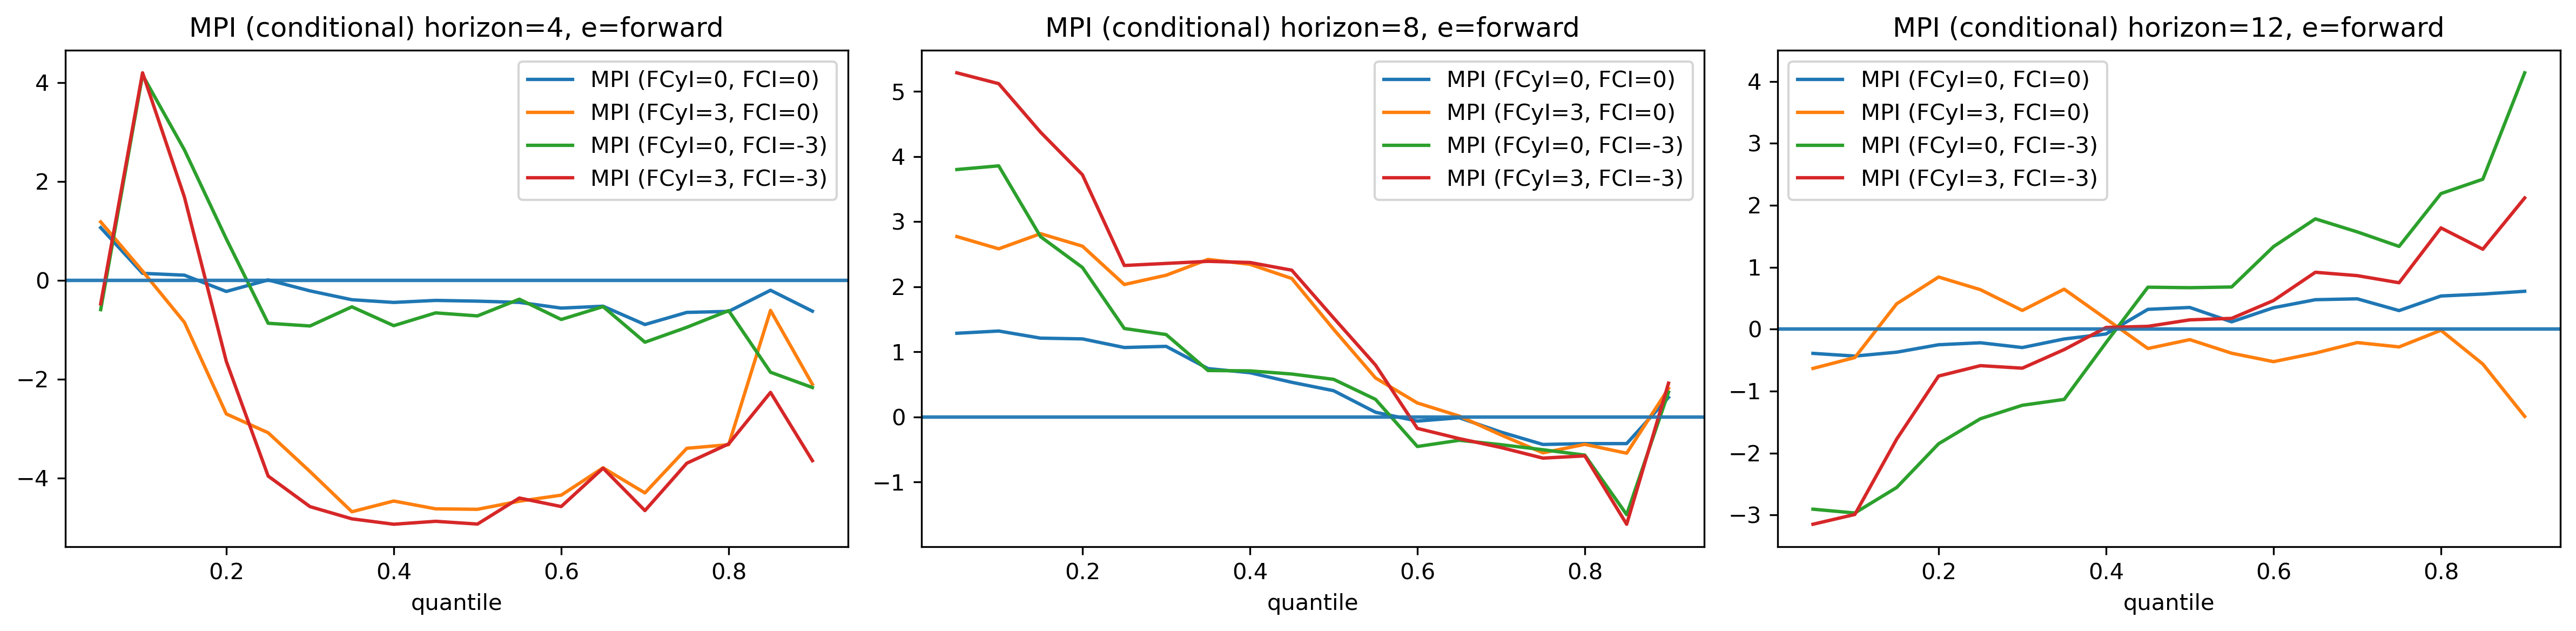
\includegraphics[width=1\textwidth, angle=0]{../Figures/arm_MPI_cond_coeff_quantiles.png}  
    \caption{Local model conditional Macroprudential Policy Index coefficients. Estimated quantile regression coefficients for horizons 4, 8 and 12.}
    \label{fig:arm_MPI_cond_coeff_quantiles}%
\end{figure*}

Short-term effects highlight the negative impact that macroprudential policy can have on median GDP growth, which is essentially the short-term cost of macroprudential on future GDP growth. On the other hand, the long-term results suggest, that in the longer term, the tail of GDP distribution shrinks significantly, while significantly benefitting the right tail of distribution. The rightmost chart in \autoref{fig:arm_MPI_cond_coeff_quantiles} also suggests that macroprudential policy is most effective during periods of low financial stress (red and green lines in the chart). However, if such periods coincide with excessive credit growth or asset price surges, the short-term costs to growth will be higher (coefficient value for median on red line in leftmost chart). Nonetheless, these conditions also lead to the most significant reduction of risks in the medium term.





\section{Macroprudential policy stance}
\subsection{Distance-to-tail approach}
\label{sec:dtt}
The goal of stance assessment is to assist macroprudential policymakers in making informed decisions. Put simply - Macroprudential decision making is based essentially on comparing the systemic risk level in the system with its resilience level, which includes also the impact of previous policy decisions. And if there is inconsistency there, the policymaker should be concerned if the source of those inconsistencies lie in financial system or are outside of it. The distance-to-tail approach achieves this by quantifying it and disaggregating its sources of systemic risk by the nature.  As was discussed in previous parts, the distance-to-tail metric is the difference between the median and tail (5\% quantile) of the fitted conditional GDP distribution. \autoref{fig:distance_to_tail_decomposition} depicts Armenia's estimated distance-to-tail over time. An increase of this indicator signals the buildup of vulnerabilities and gives a hint that policy action should supposedly be in tightening direction. What is truly important is the reason behind every move of this metric, as it can be conditioned by factors outside financial system, which, naturally should be out of the focus of macroprudential policy. Put another way, the latter should be concerned by the risks origination and/or amplification within the financial system. That is why, the mechanical rise of this metric is not solely enough for a policy action: it should be due to excessive risk accumulation (rise of FCyI) or high stress levels (rise of FCI) in order to be addressed by macroprudential policy. To address this issue, \autoref{fig:distance_to_tail_decomposition}  represents also the decomposition of the distance-to-tail ratio. For the sake of simplicity, some indicators, like capital surplus and liquidity position are not shown.
% Figure 10 misses the description of the yellow line, whether one should look at the right axis or the left one.
\begin{figure*}[!ht]
    \centering
    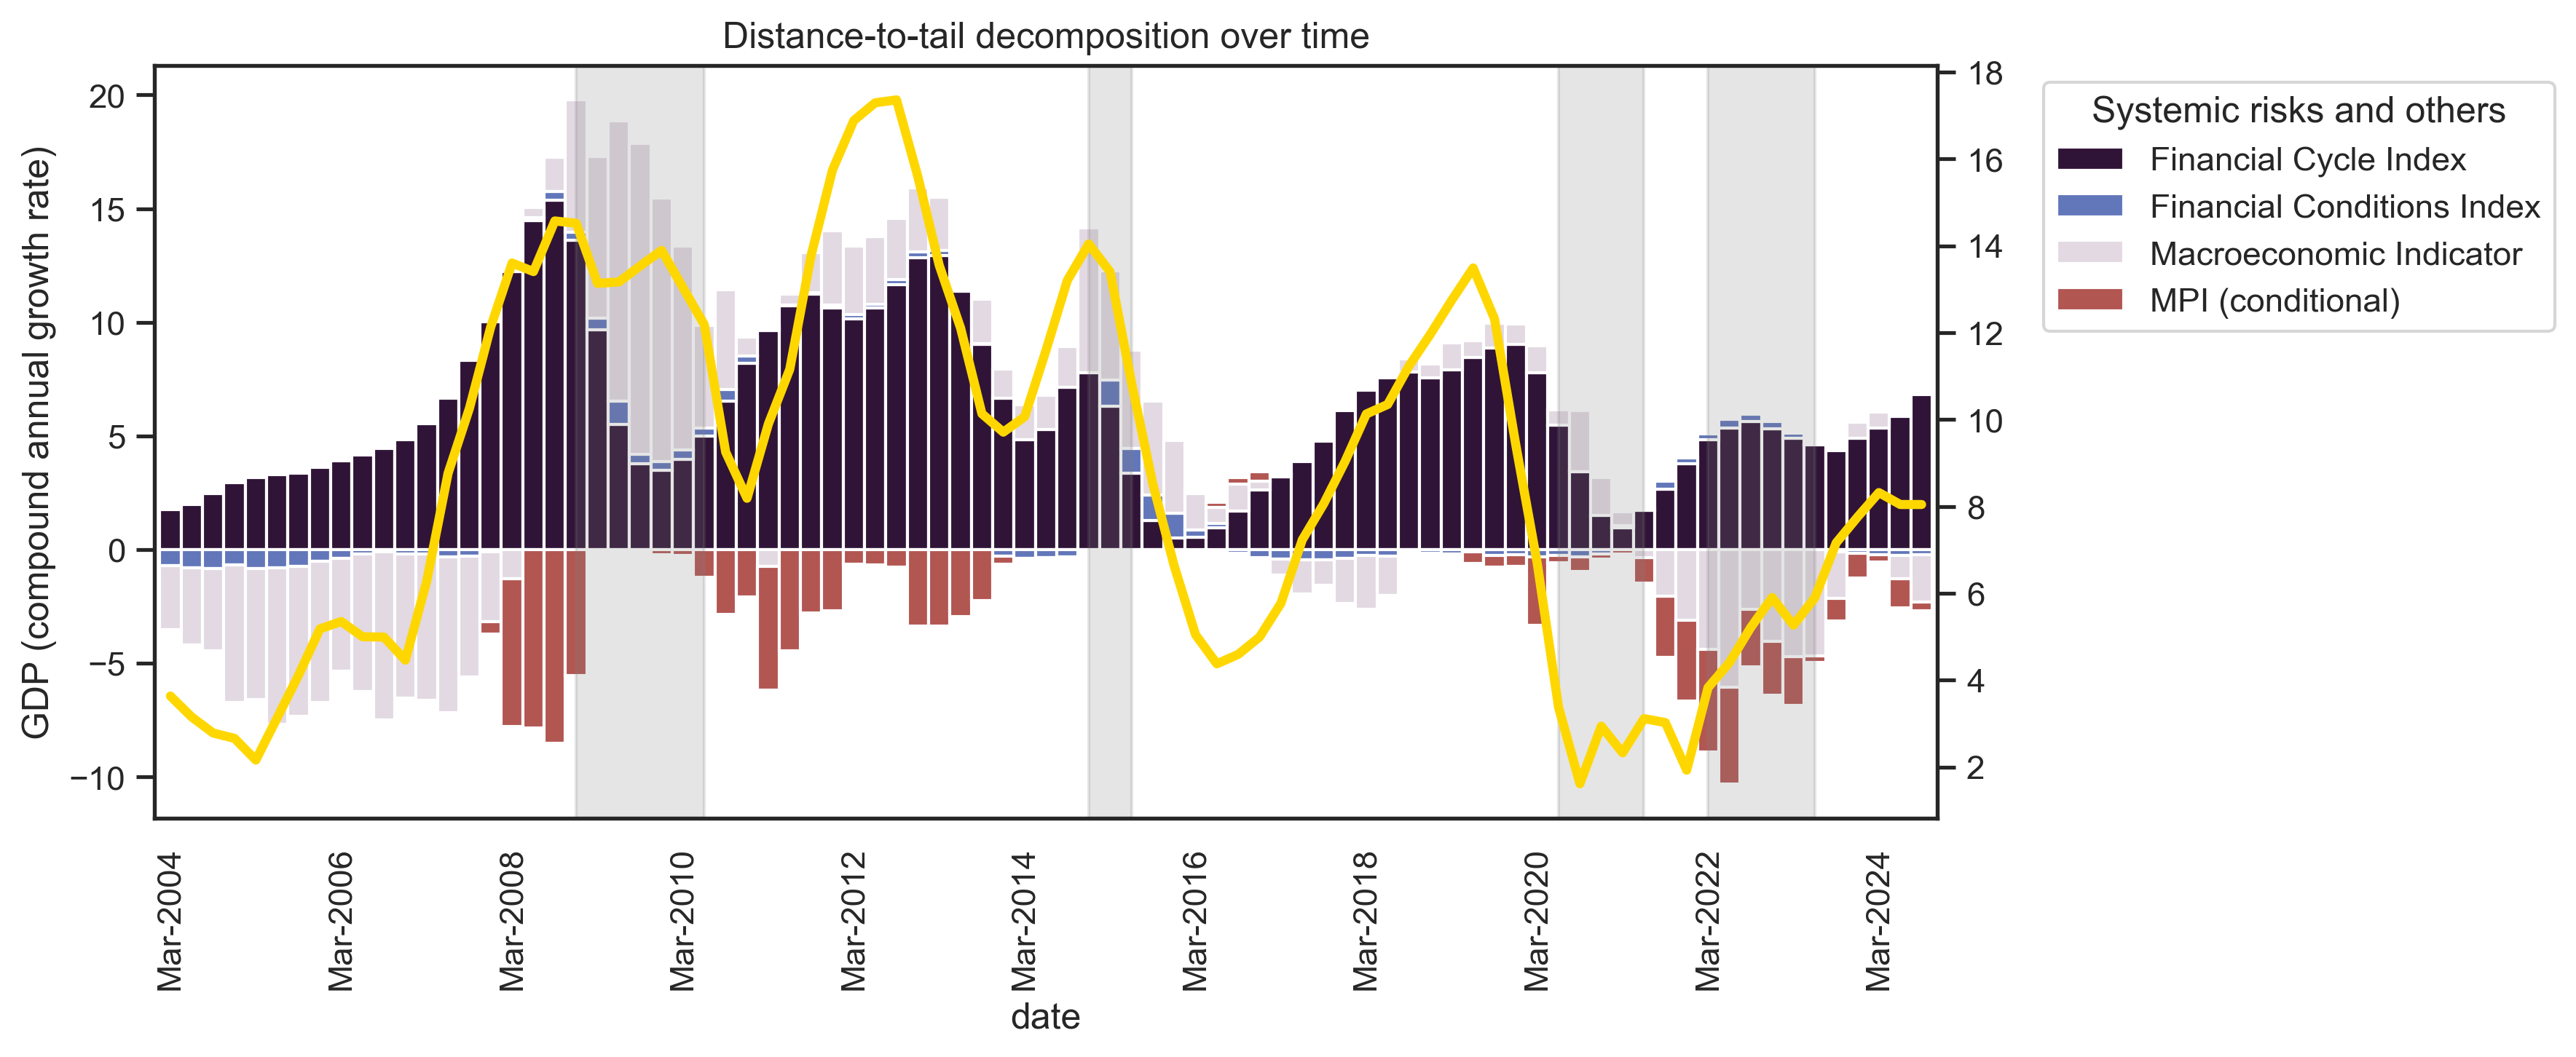
\includegraphics[width=0.9\textwidth, angle=0]{../Figures/distance_to_tail_decomposition.png}    
    \caption{Yellow line represents the distance-to-tail metric over time, and the colored bars are its components}
    \label{fig:distance_to_tail_decomposition}%
\end{figure*}
\begin{figure*}[!ht]
    \centering
    
\includegraphics[width=0.9\textwidth, angle=0]{../Figures/distance_to_tail_changes_before_crises.png}  
    \caption{Changes in distance-to-tail and the buildup of systemic risks before major economic disturbances.}
    \label{fig:distance_to_tail_changes_before_crises}%
\end{figure*}
\begin{figure*}[!ht]
    \centering
    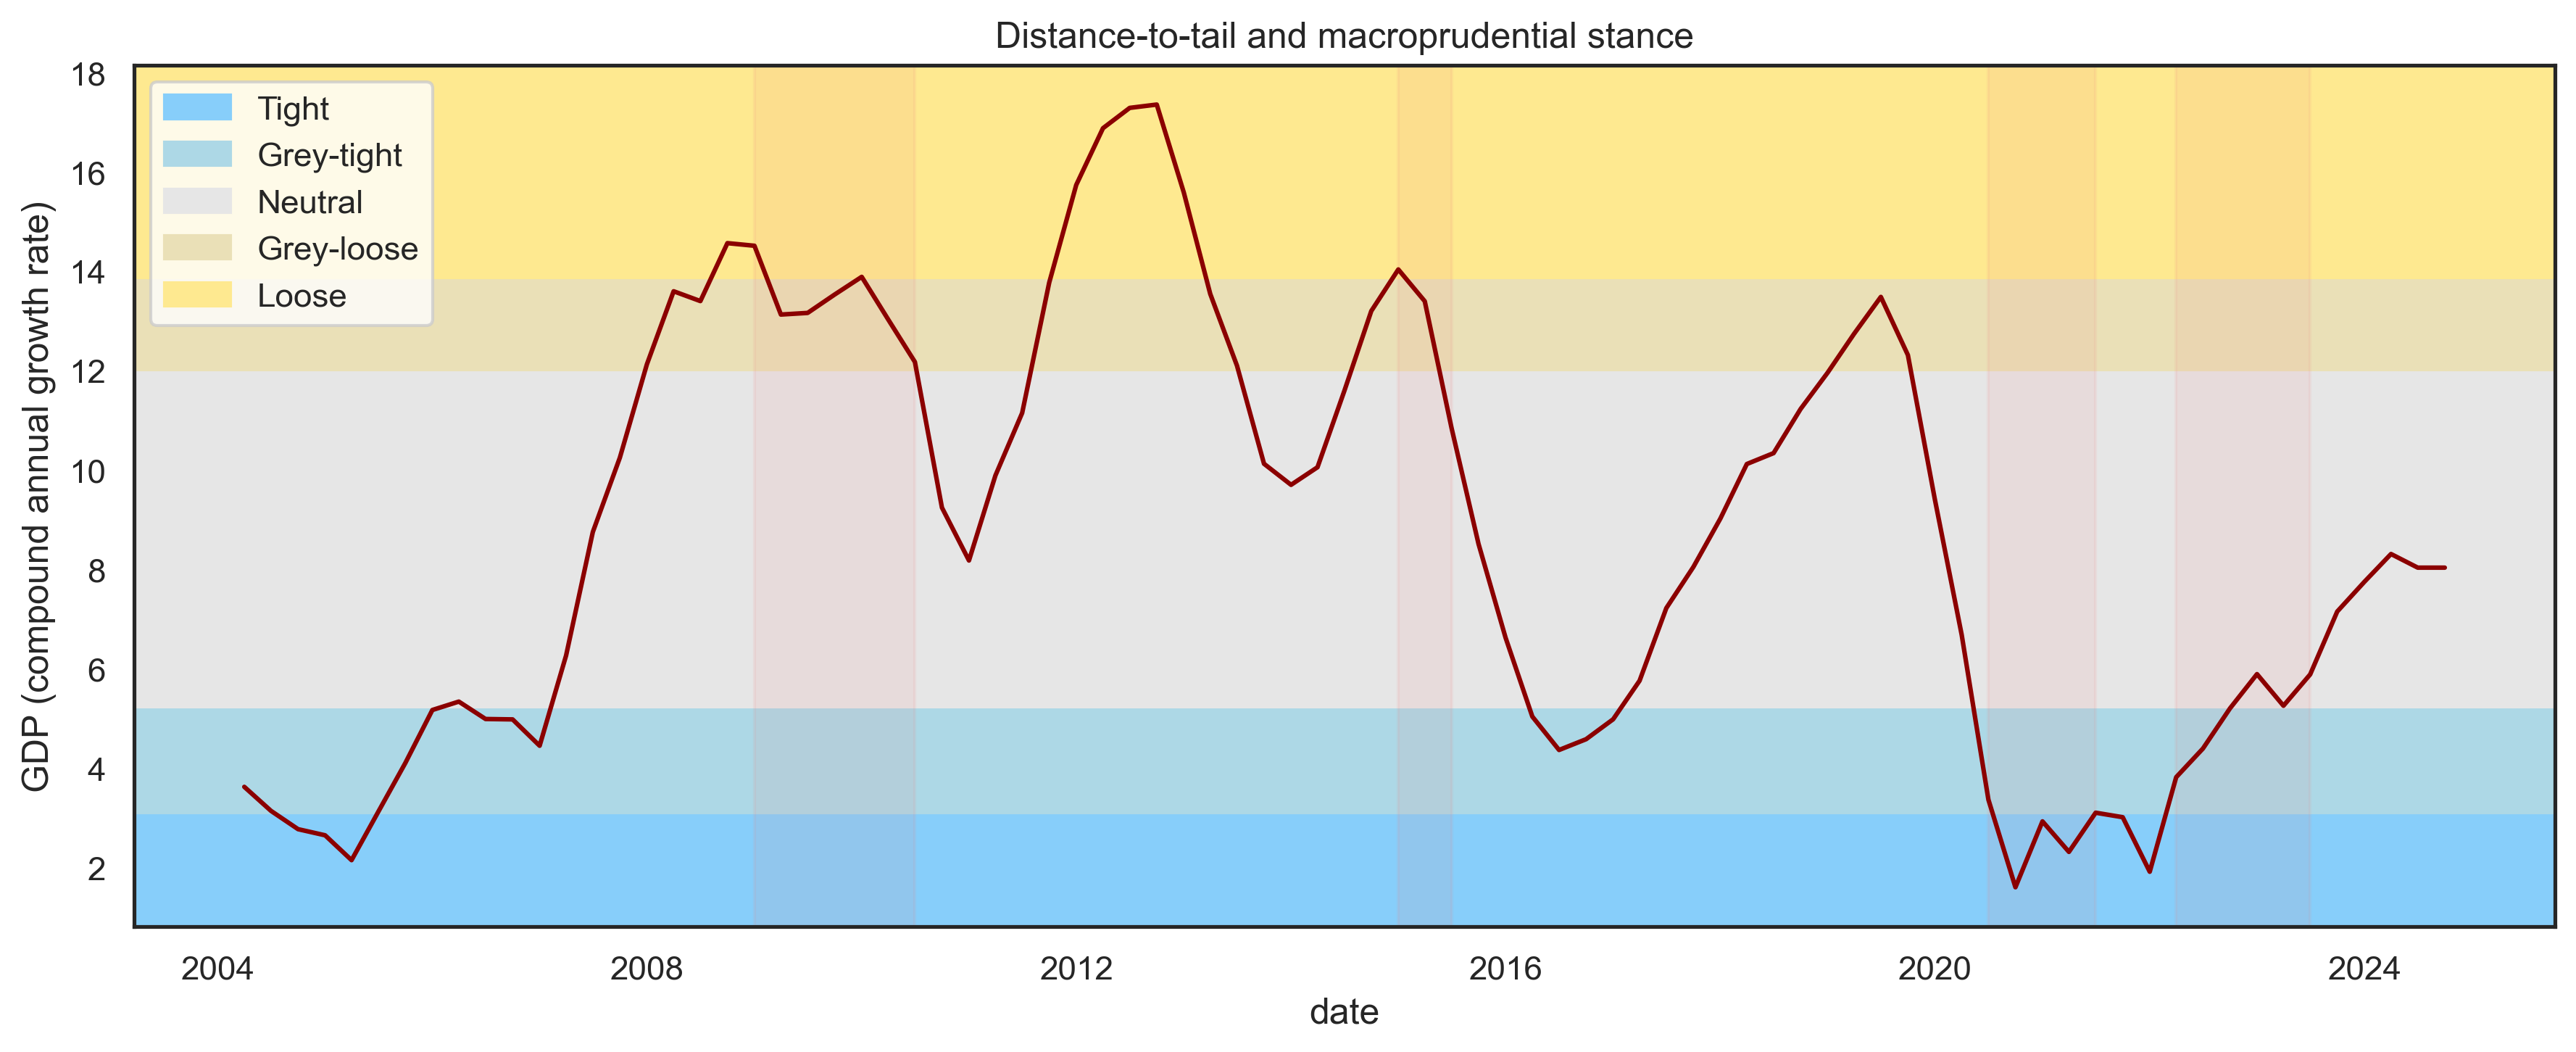
\includegraphics[width=0.9\textwidth, angle=0]{../Figures/distance_to_tail_stance.png}   
    \caption{Estimated distance-to-tail and the macroprudential stance assessment over time. The boundaries describe the 10th, 30th, 70th, and 90th percentiles of the distance-to-tail distribution.}
    \label{fig:distance_to_tail_stance}%
\end{figure*}

The results demonstrate that financial vulnerabilities follow a cyclical pattern, while financial stress tends to have smaller and less persistent impact (it is important to note, that the terms FCyI and FCI also include the interactiuon terms). Macroprudential policy actions mostly contribute to a reduction of risks. Finally, the influence of macroeconomic events on systemic risks is minimal, as they tend to shift the entire GDP growth distribution uniformly, showing little heterogeneity in their effects.

To examine the performance of the distance-to-tail metric for crisis periods we compare systemic risks in Armenia before four major economic disturbances in \autoref{fig:distance_to_tail_changes_before_crises}. Prior to the 2007-2009 financial crisis, there was a significant buildup of financial vulnerabilities, along with the accumulation of other risks that could intensify economic downturns. Indeed, during that period Armenia saw its financial intermediation rising sharply from ~7\% in 2005 to 23-24\% just before crisis. This rapid growth might have been due to some sort of catch-up process, but also due to rapid risk accumulation, which is correctly pointed by the model result. The decline of this indicator during 2014-2015 Russian oil crisis was conditioned by different set of circumstances, mainly by worsening macroeconomic environment on the one hand, and restrictive macroprudential policy on the other (in the midst of the shock, the CBA sharply raised provisioning rates of local currency denominated deposits to address local currency devaluation pressures). Before the Covid-19 shock and the Nagorno-Karabakh war, we observe a moderate increase in Financial cycle index, which was abruptly hit by the external shock. Lastly, the period leading up to the Russo-Ukrainian war overlaps with the Nagorno-Karabakh conflict, during which Armenia experienced a downturn in the financial cycle.

The distance-to-tal metric itself does not indicate the threshold where the policymaker should start to act. However, \citep{esrb2021} suggest simple yet effective way to get threshold levels for both directions of the policy, which are based on specific percentiles of its historical series. The stance metric alongside these thresholds is presented in \autoref{fig:distance_to_tail_stance}. When this value exceeds the 12\% distance-to-tail threshold (the 70th percentile), it signals a relatively loose stance, prompting consideration of tightening measures to maintain it at the neutral level. As of 2024Q4, the metric is at the neutral level, suggesting no immediate need for tightening actions. However, the value exhibits an upward trend, indicating growing risks in the system.

A key limitation of the distance-to-tail approach is that the selected threshold is not tied to a measure of the financial system's resilience, but rather inferred from itself. To test the reliability and robustness of this threshold we use an alternative methodology to derive it, inspired by modern portfolio theory. Using the estimated median and the distance-to-tail (Gap) from the panel quantile regression, we construct an efficient frontier\footnote{For details on the methodology behind the frontier, see \ref{appx:model_results}} across 41 countries, as shown in \autoref{fig:frontier_boundary}.
\begin{figure}[!ht]
	\centering 
	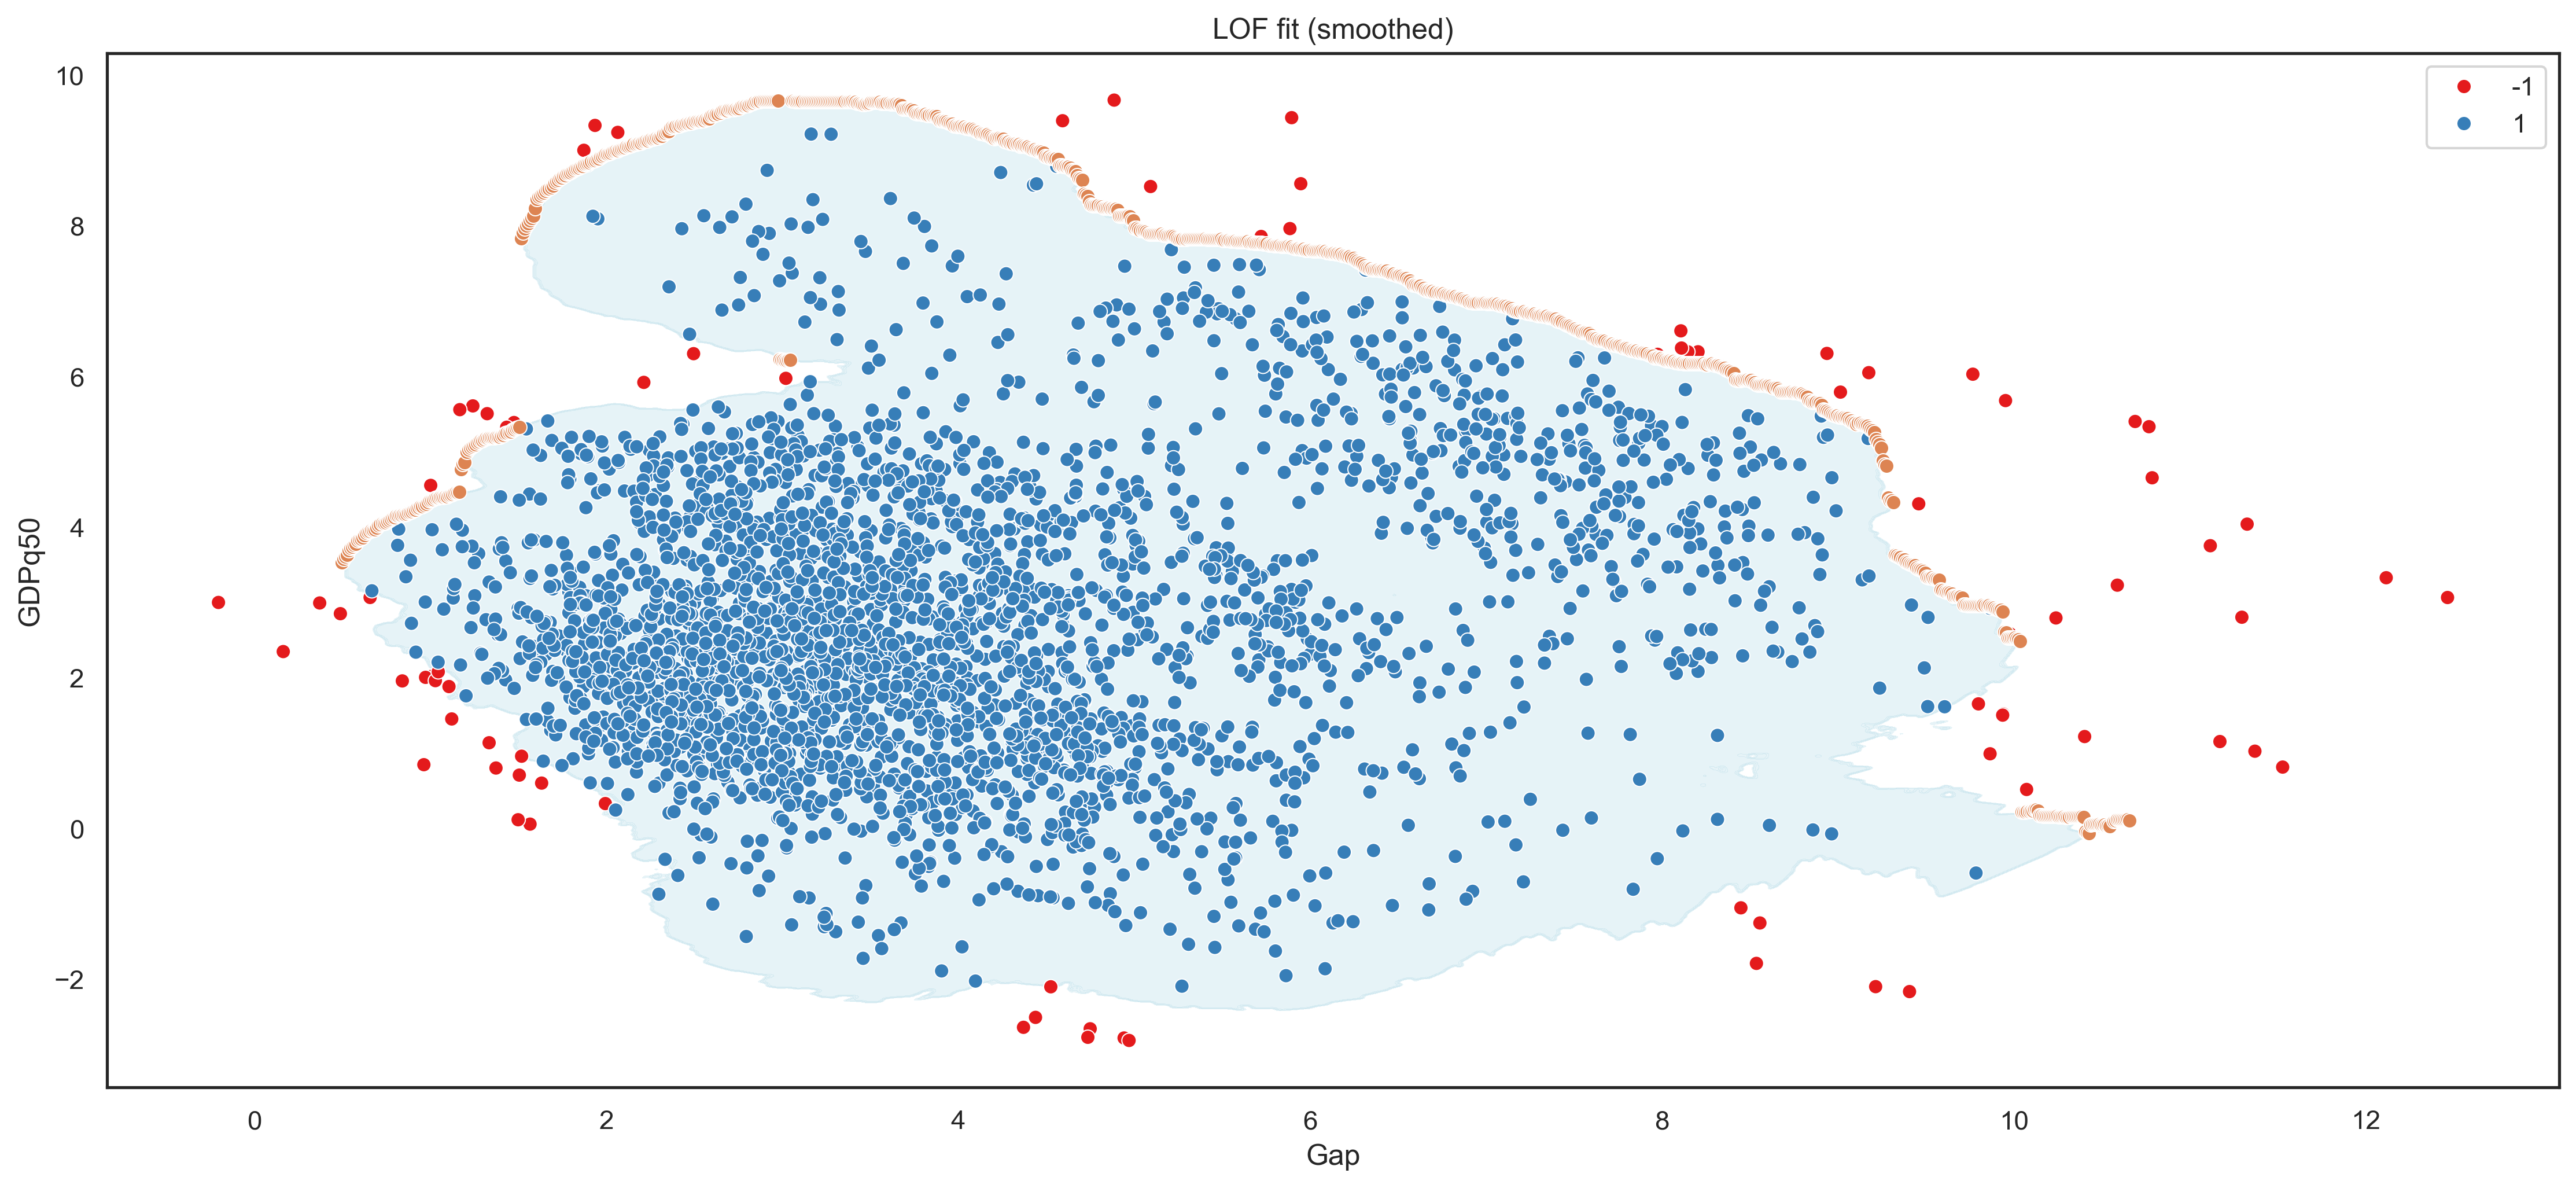
\includegraphics[width=0.9\textwidth, angle=0]{../Figures/frontier_boundary.png}	
	\caption{Local Outlier Factor (LOF) boundary based on estimates from 41 countries.} 
	\label{fig:frontier_boundary}%
\end{figure}

\autoref{fig:country_cases_that_shape_the_boundary } is a simplified version of the above chart, where a few country dots are represented and colored.

\begin{figure*}[!ht]
    \centering
    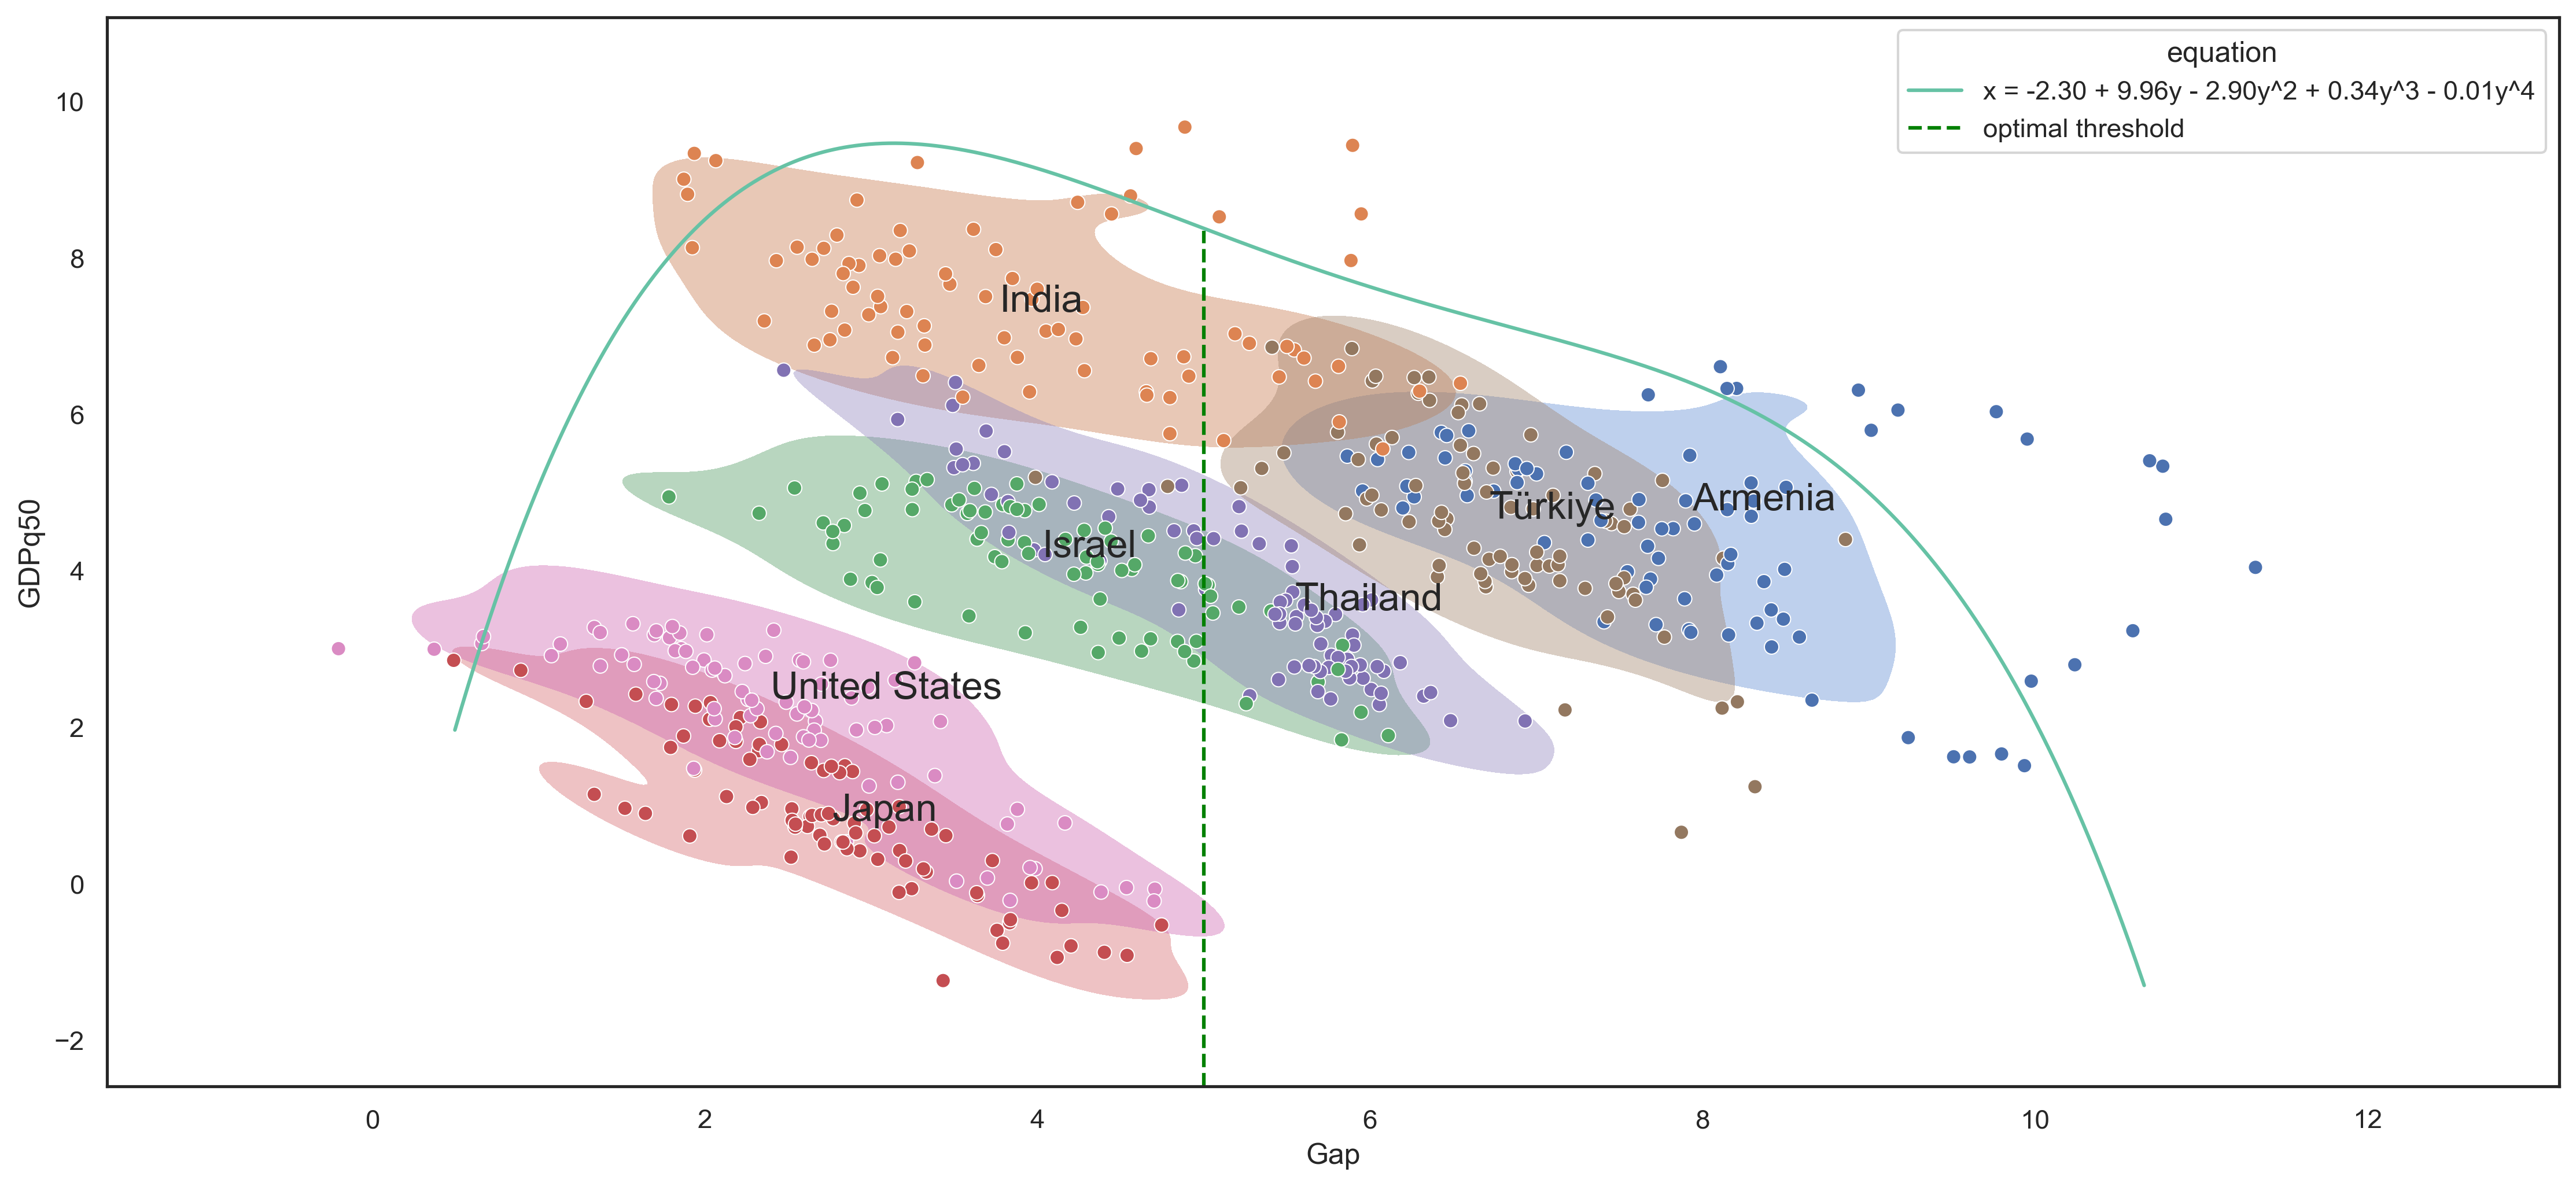
\includegraphics[width=0.9\textwidth, angle=0]{../Figures/country_cases_that_shape_the_boundary.png}   
    \caption{Fitted values for median and the tail from panel estimation and the fitted curve.}
    \label{fig:country_cases_that_shape_the_boundary }%
\end{figure*}

In this context, GDP growth represents each country's ``portfolio'', with the median as the expected return and the distance-to-tail as the associated risk. The efficient frontier illustrates that beyond a certain threshold, countries that face additional risk do not generate excess returns in proportion to those risks. If we exclude India this threshold is around 5-6\%, while including India lowers it to approximately 3\%. This finding is extremely important in this context, as it points out to the specific value for the distance-to-tail metric that should be maintained as an anchor for the neutral stance. Put another way, to be the most effective, the policymaker can take this threshold as a resistance level, over which the distance-to-tail metric should not be allowed to rise and must be brought back by tightening policy action.

\subsection{Suarez welfare approach}
Unlike the distance-to-tail approach, which considers only the distance-to-tail metric as a proxy for risk, the \citet{suarez2022} welfare function also considers the median of the distribution, enabling us to account for both the costs and benefits of the policy. The reduction of the distance-to-tail can happen by both reducing median and/or reducing the tail. A policy that reduces the median without impacting the tail would be considered unfavorable, despite lowering the distance-to-tail. However, with the welfare function, such a policy would decrease overall utility. In other words, the welfare function favors policies that are capable of improving the tail, without a reduction in the median. 
This simple yet powerful approach can assist policymaking in many ways, namely one can infer the impact of any policy action measuring and comparing possible utilities among them, and eventually figure out the optimal policy action that has the biggest utility. Central question here is the calibration of the $w$ term, depending on which the optimal policy can be quite different. There are many ways to come across an anchor value of $w$, we have used 3 methods, each of which takes some value as an anchor and finds a value of $w$  which will make a policy dicatetd by that rule to be closest to the optimal policy from Suarez function (for example, one of the approaches assumes that all the policy decisions in the past have been optimal and find an average value of $w$ that makes optimal polcy by Suarez to be closest to actual). The approximated anchor value for $w$  is around 0.11 and the details of its calibration are discussed in detail in Appendix B. 
As of 2024Q1, the conditional 1-year ahead GDP growth distribution has a median of 5.2\% and a distance-to-tail of 7.3\%. The full distribution is illustrated in \autoref{fig:arm_qr_gdp_dist}.

To present how systemic risks shape the GDP growth distribution, we compare the conditional distributions for 2023Q1 and 2024Q1 in \autoref{fig:arm_dist_optimal_policy}. It shows 3 important messages that can serve as a vital input for policymaking: first, it shows how the conditional GDP distribution is now given the risks from a year before (black line), how it will change a year after given the risks for now with no policy (red line) and with optimal policy action (green line). It can be seen from the chart, that compared to the previous year, the median has decreased by 3.5\%, while the distance-to-tail increased by 4.2\%, while with policy action, that increase in tail could be slightly smaller. Estimates suggest that a 1.5-point increase in the MPI would reduce the median by 1\% and shrink the distance-to-tail by 2.19\%, which is also the utility-maximizing policy. This is equivalent to a CCyB tightening of 0.33\%.\footnote{The conversion is performed using a simple formula: $\frac{1.5 \cdot 0.87}{4}$ For details on the ``conversion rate'' see \ref{appx:w_calibration}}

\begin{figure}[!ht]
    \centering
    
\includegraphics[width=0.9\textwidth, angle=0]{../Figures/arm_dist_optimal_policy.png}    
    \caption{GDP growth distribution conditional on systemic risks in 2023Q1 and 2024Q1. Optimal policy interaction effects are marked in green.}
    \label{fig:arm_dist_optimal_policy}%
\end{figure}

\autoref{fig:arm_dist_decomp_diff_2024Q1} further breaks down the factors contributing to this shift. The decline in the median is largely driven by macroeconomic factors, while the widening distance-to-tail reflects heightened uncertainties stemming from rising financial vulnerabilities and the indirect effects of financial stress.
\begin{figure}[!ht]
    \centering
    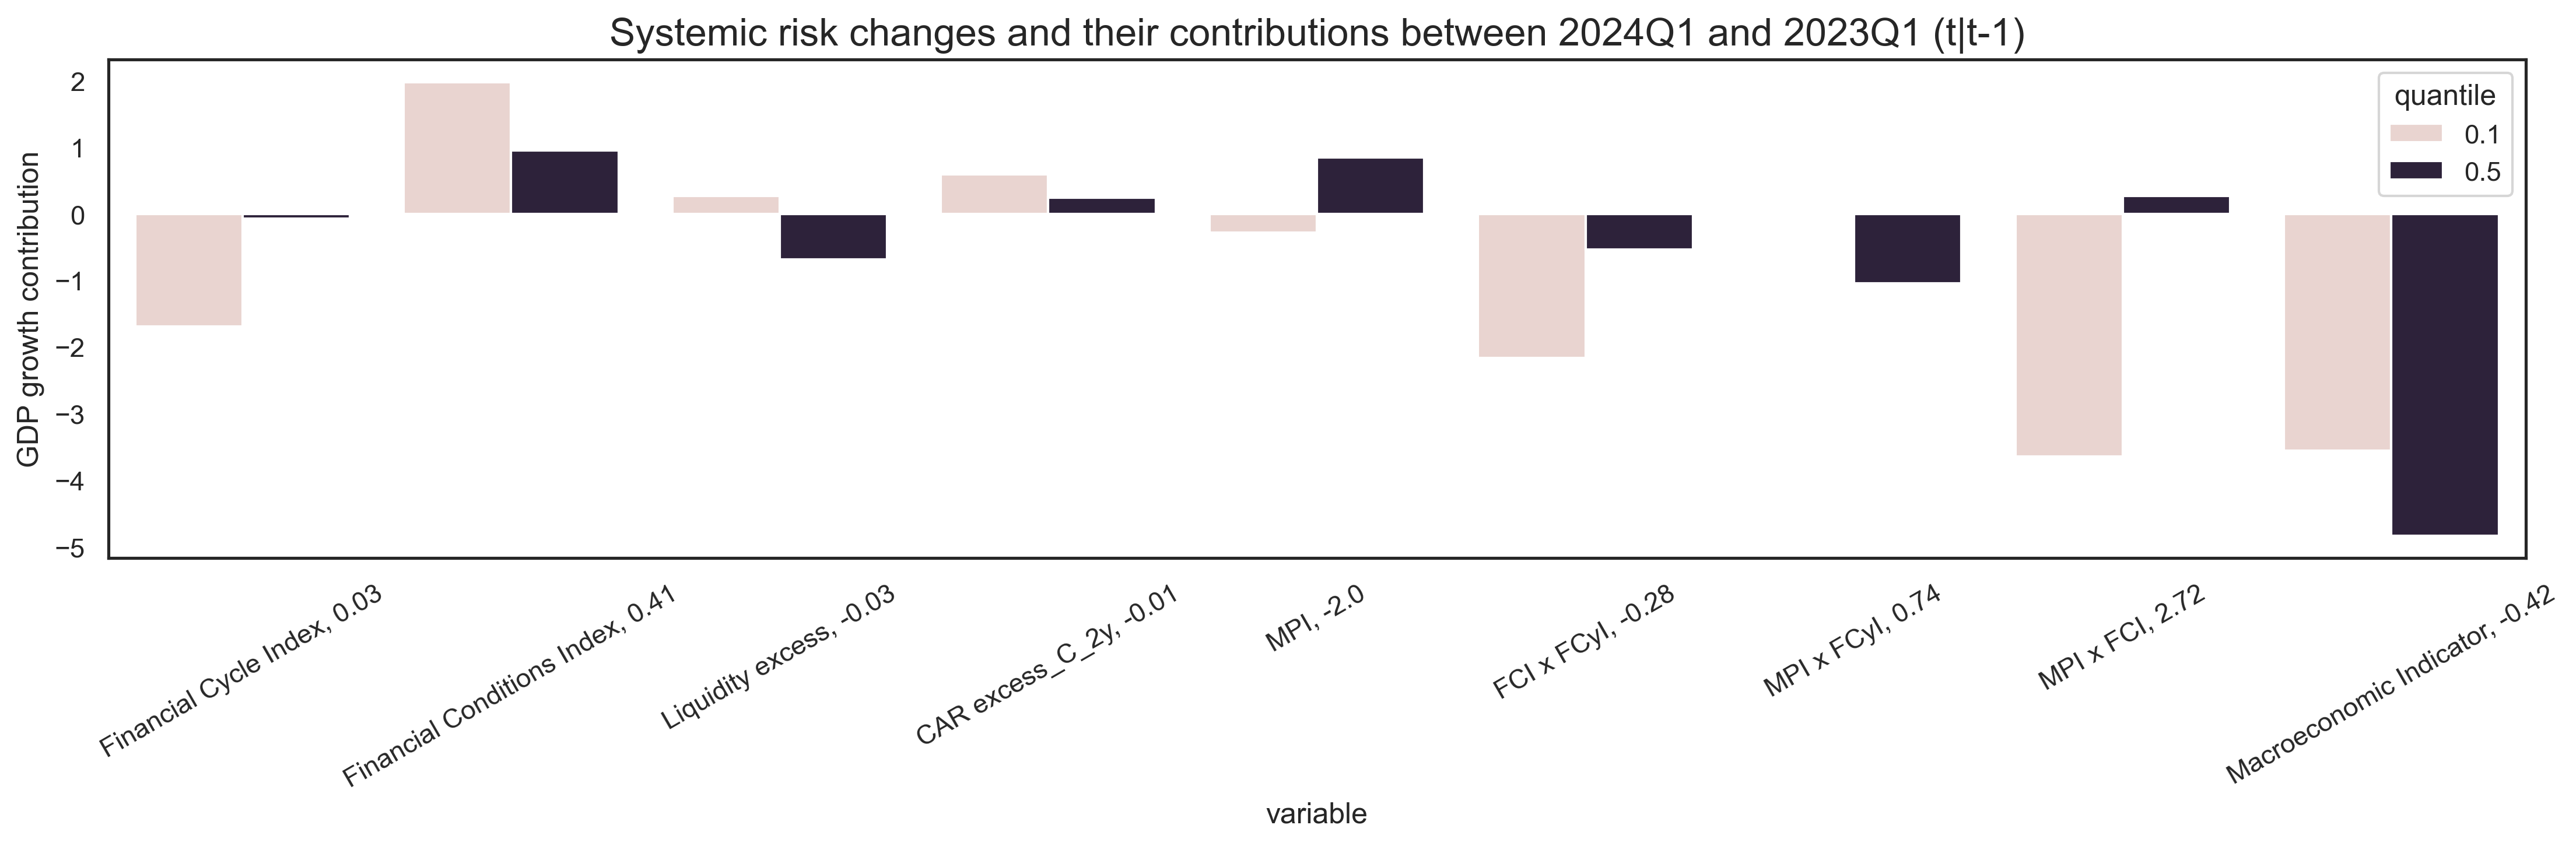
\includegraphics[width=0.9\textwidth, angle=0]{../Figures/arm_dist_decomp_diff_2024Q1.png}    
    \caption{Breakdown of factors contributing the shift of distribution.}
    \label{fig:arm_dist_decomp_diff_2024Q1}%
\end{figure}

When comparing the results from both approaches, it is apparent that they provide different conclusions. We do not view one approach as inherently superior to the other, but instead stress the importance of policymakers considering both perspectives. Each approach highlights distinct dimensions of systemic risks and policy impacts, which together provide a more comprehensive understanding of the financial system and the macroprudential stance.

\subsection{Policy simulation using the model results}
As was discussed previously, the benefits of Macroprudential policy actions are twofold: first, they enhance the resilience of the system to future possible shocks, and second they have potential to moderate the cycle, that is - to impact the size of future shocks, by curbing risky lending, etc.
To test the model we have constructed a conterfactual-like scenario for the next 20 quarters, assuming, that first half of it is a stable time and the second half is when the shock hits. At the beginning we follow the Suarez welfare approach, which taking into account current actual environment, suggests a little tightening of the policy. Then, 3 years later we assume the shock hits (we have constructed a COVID-19 like shock), and the policymaker releases the buffers (by the same amount).
\begin{figure}[!ht]
    \centering
    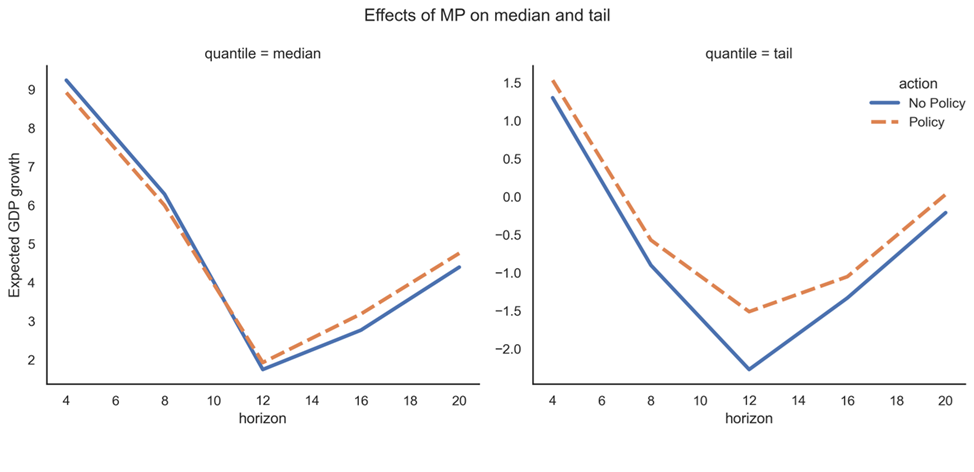
\includegraphics[width=0.9\textwidth, angle=0]{../Figures/policy_simulation.png}    
    \caption{Possible paths of GDP median and tail during the scenario horizon.}
    \label{fig:policy_simulation}%
\end{figure}
\begin{figure}[!ht]
    \centering
    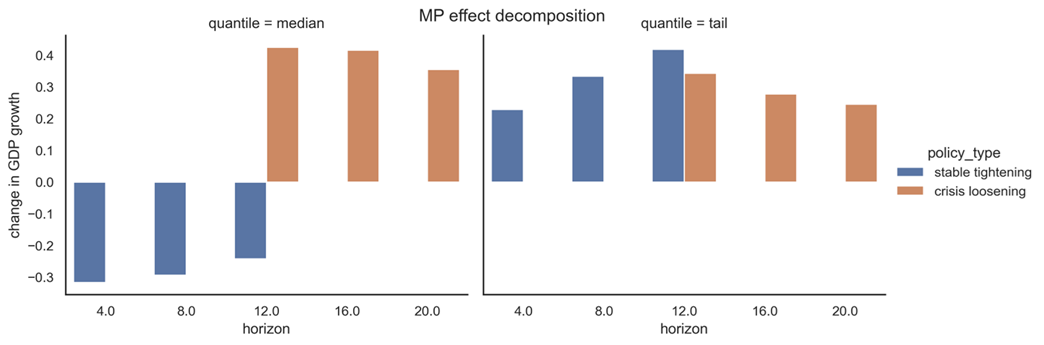
\includegraphics[width=0.9\textwidth, angle=0]{../Figures/policy_simulation_decomposition.png}    
    \caption{This figure is actually the difference between the median and the tail represented in previous chart.}
    \label{fig:policy_simulation_decomposition}%
\end{figure}

\autoref{fig:policy_simulation} and \autoref{fig:policy_simulation_decomposition} present the results. It can bee seen that initial tightening negatively impacts median GDP growth, simultaneously taming the risky tail (blue bars in \autoref{fig:policy_simulation_decomposition}). Then, when the shock hits and the policy is loosens, both median rises and the tail shrinks (orange bars in the same chart).
The results of this simple exercise seem straghtforward and natural, but still, we think that to actually have impact on policymaking, the model results still need to be calibrated with historical data, which is very scarse now due to little history of active macroprudential policy.


\section{Conclusion}
This paper quantifies the buildup of systemic risks in the Armenian economy, differentiates between those risks and considers their effects on future output growth. It also measures the impact of macroprudential policy on systemic risks and uses two approaches to derive the macroprudential stance. By employing both panel and localized models, the study ensures robust results, accounting for the nonlinear dynamics of systemic risks and policy measures. The framework integrates financial cycles, financial conditions, liquidity and capital risks, macroeconomic factors, and their interactions with macroprudential policy, while also considering the associated costs of the policy.

The findings reveal that the lag between systemic risk buildup and materialization is shorter in Armenia compared to other countries, with financial vulnerabilities following a cyclical trend and financial stress emerging more abruptly. Macroprudential policy affects the resilience of the system and is most effective during periods of low financial stress. The most significant risk reductions occur when tightening policies are applied during phases of rapid credit growth, however, this comes with larger short-term costs. Historically, the impact of the policy on financial vulnerabilities is much stronger than on financial stress.

As a small, open economy, Armenia's systemic risks are more sensitive to external shocks, but these externalities affect the entire output growth distribution rather uniformly. This suggests that while external shocks are a concern, their direct impact on systemic risks remains small.

Using the distance-to-tail approach, we estimate that a policy tightening threshold of around 7\% is appropriate for Armenia, whereas cross-country comparisons suggest a range of 5-6\%.\footnote{For details, please see \autoref{sec:dtt}} Additionally, when considering the welfare function approach, we estimate that the historical relative risk aversion in Armenia is around 3.57\footnote{For details, please see \ref{appx:w_calibration}} and offer insights on how to refine policy decisions.


\section*{Acknowledgements}
We extend our gratitude to Ashot Nanyan from the Financial Stability Directorate, Central Bank of Armenia (CBA), for his valuable suggestions and constructive discussions. We also thank our colleagues, Tatul Hayruni, Gevorg Minasyan and Aleksandr Shirkhanyan from the Economic Research Department at the CBA for their insightful comments. Special thanks to Vladimir Asriyan (Barcelona School of Economics) for his feedback and ideas on enhancing the Growth-at-Risk framework.


\section*{Data and code availability}
All scripts used for data preparation, model estimation, and figure generation are publicly available at 
\url{https://github.com/vlad-yeghiazaryan/armenian-gar}. Access can be obtained upon request from the corresponding author.

\newpage

% References
\bibliographystyle{plainnat}
\bibliography{references}


\newpage

\begin{flushleft}
    \LARGE\textbf{Appendices}\par
\end{flushleft}

\vspace{1cm}

\appendix

\section{Suarez welfare function}

\renewcommand{\thefigure}{\thesection.\arabic{figure}}
\setcounter{figure}{0}

\renewcommand{\thetable}{\thesection.\arabic{table}}
\setcounter{table}{0}


\label{appx:suarez}
One of the main advantages of GaR is that it is measured in the same units as GDP growth. This makes the comparison between the two very straightforward. Yet compared to monetary policy, the macroprudential policy literature still lacks explicit design rules. \citet{suarez2022} fills this gap by suggesting a welfare function that ``rewards expected GDP growth and penalizes the gap between expected GDP growth and GaR''. To derive this welfare function from microfoundations, the following steps are used.
First, let $Y$ denote GDP and $y$ the GDP growth rate:
\begin{equation}
    \label{eq:gdp_growth_theory}
    Y = (1+y)Y_0
\end{equation}

Now let us assume that there is a representative agent with a local coefficient of absolute risk aversion $\lambda(Y_0)$ at $Y=Y_0$. Then we can express the utility function as one exhibiting constant absolute risk aversion (CARA) with $\lambda(Y_0)$, so that:
\begin{equation}
    \label{eq:utility_theory}
    U(Y) = -\exp{\left(\lambda(Y_0)Y\right)}
\end{equation}

If we insert \autoref{eq:gdp_growth_theory} in \autoref{eq:utility_theory}, and perform a monotonic transformation, we get:
\begin{equation}
    \label{eq:utility_growth_rate_theory}
    u(y) = -\exp{\left(\lambda(Y_0)Y_0y\right)} = -\exp{\left(\rho_0 y\right)}
\end{equation}
In \autoref{eq:utility_growth_rate_theory} $\rho_0=\lambda(Y_0)Y_0$ describes the agent's coefficient of relative risk aversion at $Y_0$. If we assume GDP growth is normally distributed, so that $y\sim\mathcal{N}(y_m,y_s^2)$, then using the known moment functions we can write the agent's expected utility as:
\begin{equation}
    \label{eq:utility_expectation}
    \mathop{\mathbb{E}}\left[u(y)\right] =  -\mathop{\mathbb{E}}\left[\exp{\left(\rho_0 y\right)}\right] = -\exp{\left(-\rho_0 y_m + \frac{1}{2}\rho_0^2 y_s^2 \right)}
\end{equation}
Indirectly, \autoref{eq:utility_expectation} can also be described as: 
\begin{equation}
    \nu = y_m - \frac{\rho_0}{2}y_s^2 
\end{equation}
\begin{equation}
    y_s = \frac{y_c-y_m}{\Phi^{-1}(c)}
\end{equation}
\begin{equation}
    \nu = y_m - \frac{1}{2}\frac{\rho_0}{\left(\Phi^{-1}(c)\right)^2} (y_c - y_m)^2 
\end{equation}
Finally, by reordering some terms and assigning $w=\frac{\rho_0}{\left(\Phi^{-1}(c)\right)^2}$, which we can interpret as the aversion for financial instability, we derive the social welfare function proposed by \citet{suarez2022} in \autoref{eq:suarez_W}.

The limitations of this function are embedded in its assumptions. Since most GDP growth distributions are not normally distributed this makes the function sensitive to the choice of quantile $c$. Additionally, even if $c$ is chosen correctly, the value for $\rho_0$ and consequently $w$ is up to the policymaker. Nevertheless, this function can still serve as a good basis for policy recommendations since it offers a means to perform a cost-benefit analysis for the effects of macroprudential policy.

\section{w calibration results}

\renewcommand{\thefigure}{\thesection.\arabic{figure}}
\setcounter{figure}{0}

\renewcommand{\thetable}{\thesection.\arabic{table}}
\setcounter{table}{0}


\label{appx:w_calibration}
This section discusses the calibration procedure used to derive a representative value for $w$, the aversion for financial instability from the \citet{suarez2022} welfare function. For any arbitrary value of $w\in(0,\inf)$, it is possible to simulate an optimal policy path $\vec{p}_w$ (see \autoref{fig:arm_policy_simulation_interaction}). Using simple rules, we define 3 preferred policy paths: $\vec{p}_h$, $\vec{p}_b$, and $\vec{p}_c$. The $\vec{p}_h$ path assumes that the historical macroprudential policy of Armenia is the optimal path, in other words, all the policy decisions made so far have been the optimal ones. This assumption may seem unrealistic and indeed it is unrealistic, but here we need and anchor to calibrate the $w$ parameter, and that assumption simply assumes that the future decisions of the policymaker will have the same logic as before. The $\vec{p}_b$ path follows the CCyB rule defined by the Basel Committee \citep{basel2010}, using the credit-to-GDP gap to arrive at optimal values for CCyB. Here the problem is that we use a general macroprudential policy variable, whereas this rule strictly sticks to the specific tool of Macroprudential policy, and we need to brigde those two. According to estimates performed by \citet{esrb2021}, a ``capital-based macroprudential policy corresponds to a CET1 capital of 0.87 of risk-weighted assets''. Using this ``conversion rate'' we are able to map the CCyB rule to macroprudential policy actions and generate the Basel preferred policy path $\vec{p}_b$. The $\vec{p}_c$ path follows the same logic as $\vec{p}_b$, except for the CCyB values it uses the rule defined by the Czech National Bank (CNB). This rule is defined as a piecewise function that maps different phases of the financial cycle to CCyB decisions \citep{cnb2023}. After applying the ``conversion rate'' we end up with the policy path $\vec{p}_c$. The historical CCyB policy measures for the Basel and CNB methods are presented in \autoref{fig:arm_ccyb_simulation}.
\begin{figure}[!ht]
	\centering 
	
\includegraphics[width=0.9\textwidth, angle=0]{../Figures/arm_policy_simulation_interaction.png}	
	\caption{Policy path simulation given an arbitrary value for w.} 
	\label{fig:arm_policy_simulation_interaction}%
\end{figure}
\begin{figure}[!ht]
	\centering 
	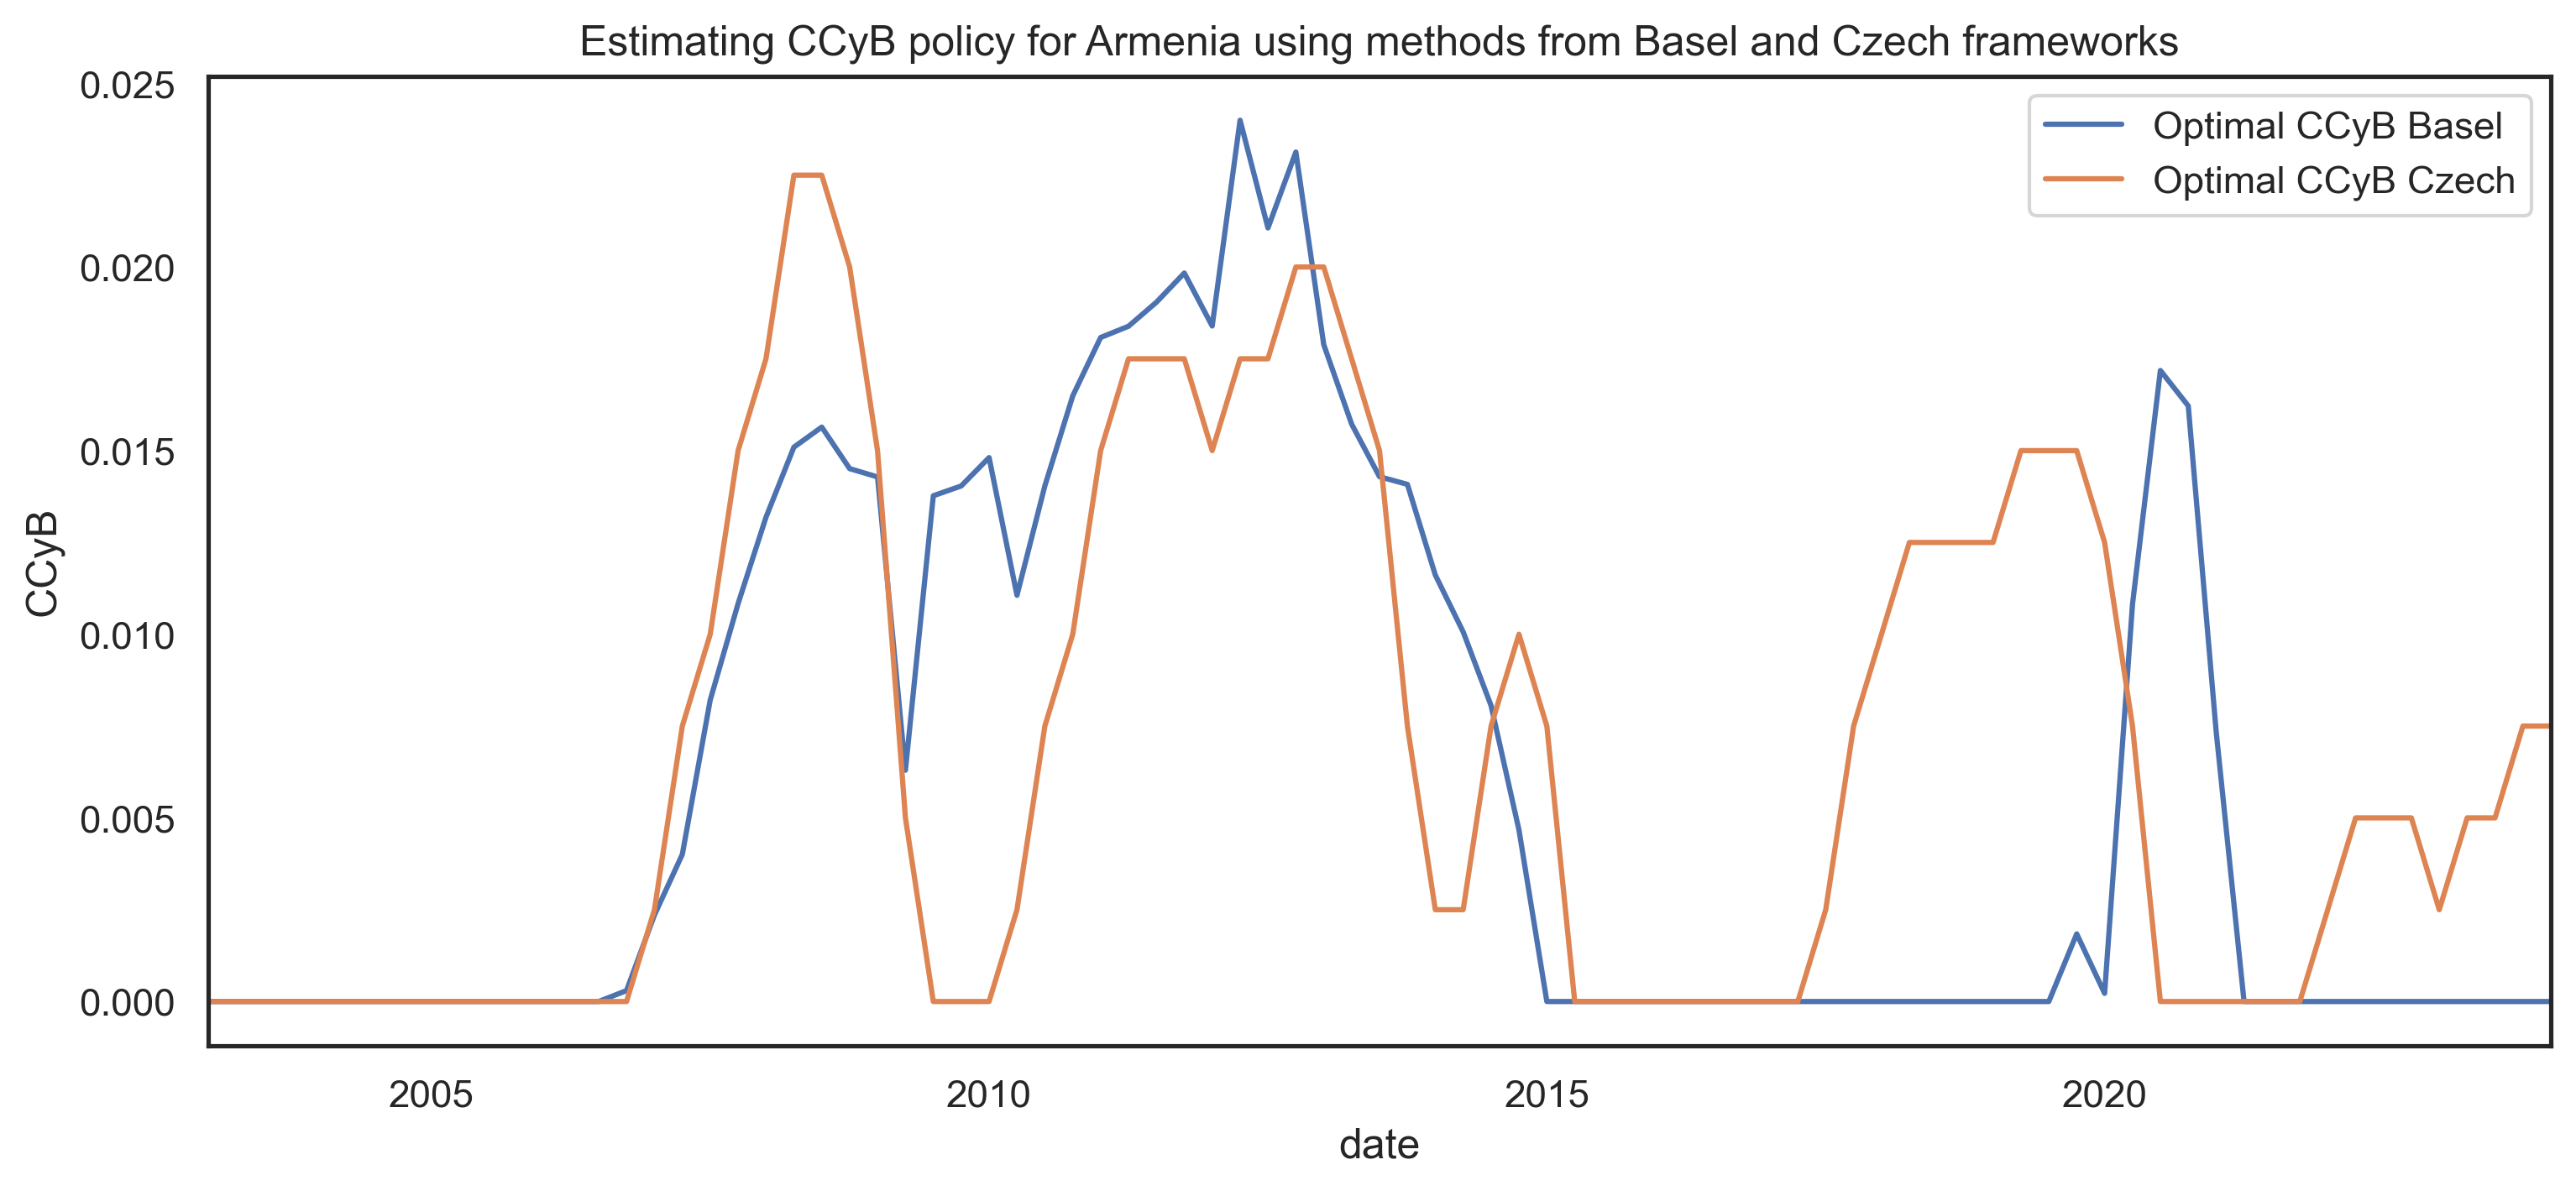
\includegraphics[width=0.9\textwidth, angle=0]{../Figures/arm_ccyb_simulation.png}	
	\caption{Optimal CCyB tightening measures derived using the Basel gap and Financial Cycle Index (CNB)} 
	\label{fig:arm_ccyb_simulation}%
\end{figure}

Next, to see which path is the most viable we compare all of the optimal paths $\vec{p}_w$ with the 3 preferred policy paths by taking the Euclidean distance between them. Put another way, we have two policy choices: policies generated by Suarez welfare function and either one of the three policies suggested above: We simply need to get the appropriate value of $w$ parameter, that makes those two closest to each other. \autoref{fig:arm_w_calibration_interaction} shows the relationship between the choice of $w$ and the 3 preferred policy paths. Using the elbow method and optimal choices from the Basel and CNB methods, we believe that 0.11 is a representative value. This is also equivalent to a relative risk aversion $\rho_0=w\left(\Phi^{-1}(c)\right)^2$ of 3.57, which is in line with the values considered in the literature \citep{cecchetti_2021}.
\begin{figure}[!ht]
	\centering 
	
\includegraphics[width=0.9\textwidth, angle=0]{../Figures/arm_w_calibration_interaction.png}	
	\caption{Euclidean distance between $\vec{p}_w$ and the 3 preferred policy paths for all values of $w$. The dotted lines show the points with the smallest distance.} 
	\label{fig:arm_w_calibration_interaction}%
\end{figure}

As a robustness check for the calibration results above, we ignore the 2 preferred policy paths and instead allow the value of $w$ to change over time. We then select the set $vect{w}$ so that $\vec{p}_{\vec{w}}$ matches almost exactly with $\vec{p}_h$. Finally, we plot the distribution for $w$ in \autoref{fig:arm_w_dynamic_dist}. The selected value of 0.11 is not significantly different from the modes of these distributions.
\begin{figure}[!ht]
	\centering 
	
\includegraphics[width=0.9\textwidth, angle=0]{../Figures/arm_w_dynamic_dist.png}	
	\caption{Distribution for the dynamic values of $w$ over time.} 
	\label{fig:arm_w_dynamic_dist}%
\end{figure}

\section{Input data and transformations}

\renewcommand{\thefigure}{\thesection.\arabic{figure}}
\setcounter{figure}{0}

\renewcommand{\thetable}{\thesection.\arabic{table}}
\setcounter{table}{0}


\label{appx:data}
\subsection{Data for the panel model}
\autoref{table:panel_stats} and \autoref{table:panel_tf_stats} illustrate summary statistics related to the panel data before and after the transformations. Variables with the prefix ``\_C'' and ``\_PctC'' describe the simple difference and percentage change difference transformations respectively. Variables with the prefix ``\_lag\_i'' indicate that the series has been shifted backward by $i$ quarters.
\begin{table}
\begin{center}
\caption{Panel summary statistics}
\label{table:panel_stats}
\scalebox{0.55}{
\begin{tabular}{lllllll}
\toprule
 & count & mean & std & min & 50\% & max \\
\midrule
GDP\_real\_growth\_1.0y & 5,084.00 & 3.22 & 4.52 & -23.37 & 2.98 & 45.60 \\
REER & 5,248.00 & 96.60 & 14.51 & 19.09 & 97.92 & 163.71 \\
Bond\_yield\_5Y & 5,248.00 & 6.47 & 5.63 & -0.99 & 5.33 & 61.15 \\
Bond\_yield\_1Y & 5,248.00 & 5.60 & 5.09 & -0.77 & 4.62 & 35.50 \\
Unemployment & 5,248.00 & 7.64 & 4.21 & 0.48 & 6.90 & 28.20 \\
CPI & 5,248.00 & 87.32 & 31.82 & 0.00 & 90.46 & 350.54 \\
Credit\_GDP\_ratio & 5,248.00 & 134.63 & 68.67 & 6.03 & 133.60 & 400.60 \\
Credit\_GDP\_gap & 5,248.00 & 0.89 & 14.49 & -107.20 & 0.87 & 80.00 \\
Liquid\_asset\_ratio & 5,248.00 & 27.76 & 23.50 & 3.46 & 23.94 & 211.54 \\
RPP\_Real & 5,248.00 & 95.07 & 34.67 & 33.32 & 96.13 & 237.65 \\
Provisions/NPL & 5,248.00 & 60.56 & 43.70 & -94.42 & 52.65 & 314.02 \\
Bank\_liabilities\_MC & 5,248.00 & 336,897,733.54 & 935,041,903.27 & 515.90 & 6,667,702.39 & 3,633,974,000.00 \\
RRE/Loans & 5,248.00 & 21.56 & 17.09 & 0.12 & 18.57 & 84.34 \\
Interest\_margin/Income & 5,248.00 & 58.42 & 16.15 & -294.33 & 59.07 & 498.61 \\
CAR\_T1 & 5,248.00 & 12.83 & 4.00 & -3.64 & 12.49 & 33.72 \\
MPI & 5,248.00 & 0.54 & 1.82 & -13.00 & 0.00 & 12.00 \\
DSR & 5,248.00 & 16.34 & 5.36 & 3.00 & 16.20 & 40.10 \\
FCI & 4,756.00 & 0.00 & 0.76 & -5.13 & 0.16 & 1.74 \\
FCyI & 4,756.00 & 0.15 & 0.14 & -0.01 & 0.11 & 0.82 \\
\bottomrule
\end{tabular}
}
\end{center}
\end{table}
\begin{table}
\begin{center}
\caption{Panel summary statistics for transformed variables}
\label{table:panel_tf_stats}
\scalebox{0.6}{
\begin{tabular}{lllllll}
\toprule
 & count & mean & std & min & 50\% & max \\
\midrule
GDP\_real\_growth\_1.0y & 5,084.00 & 3.22 & 4.52 & -23.37 & 2.98 & 45.60 \\
GDP\_real\_growth\_2.0y & 4,920.00 & 3.11 & 3.43 & -13.03 & 2.84 & 30.49 \\
GDP\_real\_growth\_3.0y & 4,756.00 & 3.16 & 3.03 & -8.39 & 2.82 & 25.84 \\
REER\_lag\_1\_normalized & 4,756.00 & 0.02 & 0.96 & -4.00 & 0.05 & 3.17 \\
Bond\_yield\_5Y\_C\_2y & 4,756.00 & -0.68 & 3.70 & -56.70 & -0.55 & 52.49 \\
Bond\_yield\_1Y\_normalized\_C\_3y & 4,756.00 & -0.28 & 0.77 & -6.37 & -0.23 & 4.92 \\
Unemployment\_normalized & 4,756.00 & -0.01 & 0.99 & -3.63 & -0.11 & 5.73 \\
CPI\_C\_1y & 4,756.00 & 2.89 & 4.10 & -54.50 & 2.16 & 72.00 \\
Credit\_GDP\_ratio\_PctC\_2y & 4,756.00 & 0.05 & 0.12 & -0.65 & 0.04 & 1.23 \\
Credit\_GDP\_gap\_PctC\_2y & 4,756.00 & -0.43 & 10.40 & -434.15 & -0.18 & 125.00 \\
Liquid\_asset\_ratio\_PctC\_2y & 4,756.00 & 0.01 & 0.16 & -0.73 & -0.00 & 1.84 \\
RPP\_Real\_PctC\_3y & 4,756.00 & 0.08 & 0.19 & -0.45 & 0.06 & 1.12 \\
Provisions/NPL\_C\_2y & 4,756.00 & 0.53 & 16.28 & -169.40 & 0.36 & 99.23 \\
Bank\_liabilities\_MC\_normalized\_C\_1y & 4,756.00 & 0.06 & 0.45 & -4.73 & 0.01 & 3.77 \\
RRE/Loans\_PctC\_1y & 4,756.00 & 0.20 & 2.11 & -0.98 & 0.01 & 57.52 \\
Interest\_margin/Income\_normalized\_C\_2y & 4,756.00 & 0.02 & 1.29 & -10.64 & 0.02 & 10.96 \\
CAR\_T1\_lag\_3\_PctC\_1y & 4,756.00 & 0.02 & 0.55 & -31.89 & 0.02 & 12.64 \\
MPI & 4,756.00 & 0.59 & 1.90 & -13.00 & 0.00 & 12.00 \\
DSR & 4,756.00 & 16.44 & 5.33 & 3.00 & 16.42 & 40.10 \\
FCI & 4,756.00 & 0.00 & 0.76 & -5.13 & 0.16 & 1.74 \\
FCyI & 4,756.00 & 0.15 & 0.14 & -0.01 & 0.11 & 0.82 \\
\bottomrule
\end{tabular}
}
\end{center}
\end{table}

\subsection{Data from the local model}
\begin{table}
\begin{center}
\caption{Local model summary statistics}
\label{table:local_stats}
\scalebox{0.7}{
\begin{tabular}{lrrrrrr}
\toprule
 & count & mean & std & min & 50\% & max \\
\midrule
GDP\_real\_growth\_1.0y & 81 & 5.5 & 7.4 & -19.8 & 6.7 & 19.1 \\
Financial Cycle Index & 85 & 0.1 & 0.1 & 0.0 & 0.1 & 0.3 \\
Financial Conditions Index & 85 & 0.0 & 0.7 & -1.3 & 0.0 & 2.4 \\
Liquidity excess & 85 & 0.2 & 0.1 & 0.1 & 0.2 & 0.4 \\
CAR excess & 85 & 0.1 & 0.1 & 0.0 & 0.1 & 0.2 \\
Mortgage stock & 72 & 0.3 & 0.4 & 0.0 & 0.2 & 1.6 \\
Mortgage flow & 72 & 0.4 & 0.6 & -0.8 & 0.2 & 1.6 \\
Mortgage interest rate & 63 & -2.1 & 0.1 & -2.3 & -2.1 & -1.6 \\
Construction loans & 77 & 0.7 & 0.6 & -0.1 & 0.5 & 3.0 \\
Real estate prices & 81 & 0.1 & 0.1 & -0.2 & 0.1 & 0.4 \\
DSTI & 77 & 0.0 & 0.0 & 0.0 & 0.0 & 0.1 \\
Macroeconomic Indicator & 85 & 0.0 & 0.3 & -1.0 & 0.0 & 0.5 \\
MP & 85 & 0.3 & 0.7 & -1.0 & 0.0 & 3.0 \\
MPI & 85 & 1.2 & 1.7 & -2.0 & 1.0 & 6.0 \\
\bottomrule
\end{tabular}
}
\end{center}
\end{table}



\section{Additional Panel and local model estimation results}

\renewcommand{\thefigure}{\thesection.\arabic{figure}}
\setcounter{figure}{0}

\renewcommand{\thetable}{\thesection.\arabic{table}}
\setcounter{table}{0}


\label{appx:model_results}
\subsection{Panel model estimation results}
The full list of countries used in the panel estimation includes Armenia, Australia, Austria, Belgium, Brazil, Chile, Colombia, Croatia, Czech Republic, Denmark, Finland, France, Georgia, Germany, Greece, Hong Kong, China, Hungary, Iceland, India, Ireland, Israel, Italy, Japan, Korea, Republic of, Mexico, Netherlands, New Zealand, Norway, Philippines, Poland, Portugal, Romania, Russian Federation, Singapore, Spain, Sweden, Switzerland, Thailand, Türkiye, United Kingdom and United States.
\begin{table}[!ht]
\begin{center}
\caption{In-sample panel quantile regression coefficients.}
\label{table:panel_coeffs}
\scalebox{0.6}{
\begin{tabular}{p{7cm}p{3cm}p{3cm}}
\hline
                                           & GDP growth, h=4, q=0.1, e=f & GDP growth, h=4, q=0.5, e=f \\
\hline
autoregressive                             & 0.0302                      & 0.1038***                    \\
                                           & (0.0276)                    & (0.0107)                     \\
FCyI                                       & -3.4029***                  & -2.0606***                   \\
                                           & (0.6489)                    & (0.3287)                     \\
FCI                                        & 0.2306*                     & 0.1166**                     \\
                                           & (0.1188)                    & (0.0593)                     \\
MPI                                        & 0.1012*                     & -0.0221                      \\
                                           & (0.0550)                    & (0.0275)                     \\
DSR                                        & -0.1543***                  & -0.1084***                   \\
                                           & (0.0274)                    & (0.0147)                     \\
Interest\_margin/Income\_normalized\_C\_2y & -0.1249**                   & -0.0268                      \\
                                           & (0.0559)                    & (0.0270)                     \\
Bank\_liabilities\_MC\_normalized\_C\_1y   & -0.8270***                  & -0.5366***                   \\
                                           & (0.1662)                    & (0.0803)                     \\
NPL\_ratio\_PctC\_3y                       & -0.1747***                  & -0.0424                      \\
                                           & (0.0562)                    & (0.0290)                     \\
Provisions/NPL\_C\_2y                      & 0.0231***                   & 0.0057**                     \\
                                           & (0.0044)                    & (0.0024)                     \\
RPP\_Real\_PctC\_3y                        & 3.6966***                   & 3.9197***                    \\
                                           & (0.4692)                    & (0.2543)                     \\
RRE\_Loans\_MC\_PctC\_1y                   & 1.3092***                   & 0.7058***                    \\
                                           & (0.1921)                    & (0.1395)                     \\
CPI\_C\_1y                                 & -0.1441***                  & -0.0532***                   \\
                                           & (0.0212)                    & (0.0109)                     \\
MPR\_log                                   & -0.2010***                  & -0.0307                      \\
                                           & (0.0539)                    & (0.0273)                     \\
Unemployment\_normalized                   & 1.0673***                   & 0.6037***                    \\
                                           & (0.0969)                    & (0.0451)                     \\
FX\_log\_C\_2y                             & 0.8575***                   & 0.5483***                    \\
                                           & (0.1767)                    & (0.0886)                     \\
Import\_Merchandise\_Price\_normalized     & -0.9196***                  & -0.4745***                   \\
                                           & (0.0833)                    & (0.0405)                     \\
FCyI x FCI                                 & 2.0863***                   & 0.9796**                     \\
                                           & (0.6735)                    & (0.3813)                     \\
MPI x FCyI                                 & -0.2048*                    & 0.0615                       \\
                                           & (0.1066)                    & (0.0614)                     \\
MPI x FCI                                  & -0.9881***                  & -0.3099***                   \\
                                           & (0.1947)                    & (0.0913)                     \\
N                                          & 4469.0000                   & 4469.0000                    \\
Pseudo-R2                                  & 0.1831                      & 0.2007                       \\
\hline \\
\multicolumn{3}{l}{* p<0.05,  ** p<0.01,  *** p<0.001}
\end{tabular}
}
\end{center}
\end{table}
\begin{figure}[!ht]
	\centering 
	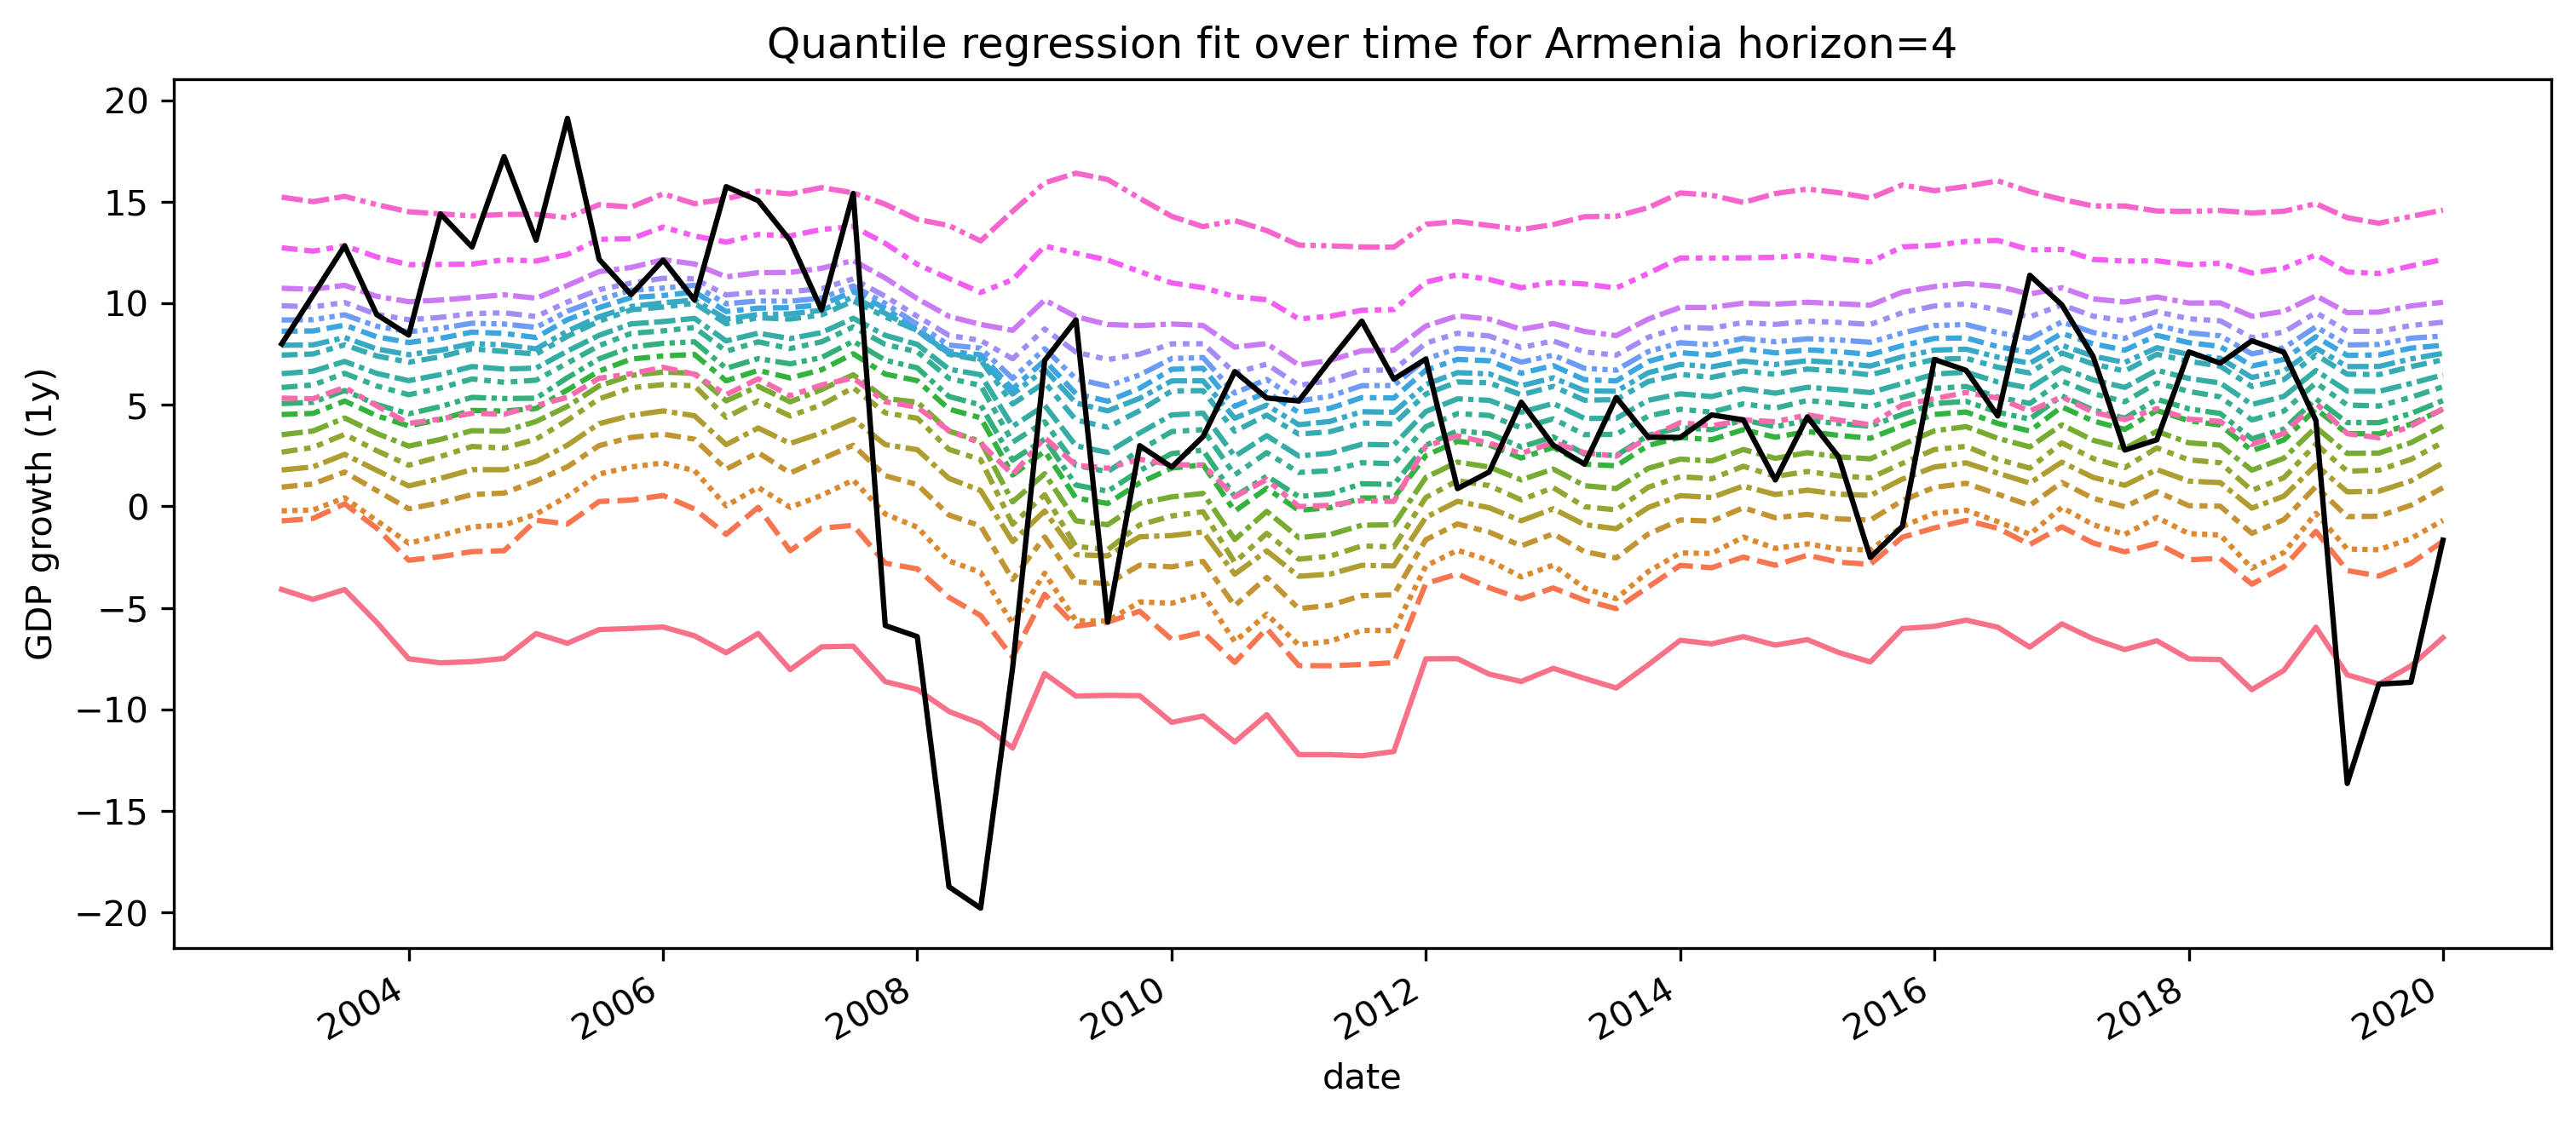
\includegraphics[width=0.9\textwidth, angle=0]{../Figures/panel_qr_prediction_for_Armenia.png}	
	\caption{Panel quantile regression one year ahead fitted values of Armenia for different quantiles.} 
	\label{fig:panel_qr_prediction_for_Armenia}%
\end{figure}

In \autoref{fig:frontier_boundary} we plot the estimated median and distance-to-tail (Gap) values. We then use the Local Outlier Factor (LOF) algorithm on the data points to compute local densities for each of the points relative to their neighbors. Points with very low density are considered to be outliers (marked in red). Using this density function we derive a boundary that best describes the efficient frontier for our risk (Gap) and reward (median) pairs. Boundary points are marked in orange. By fitting a polynomial onto these points, it is possible to derive an explicit frontier function.

\begin{figure}[!ht]
	\centering 
	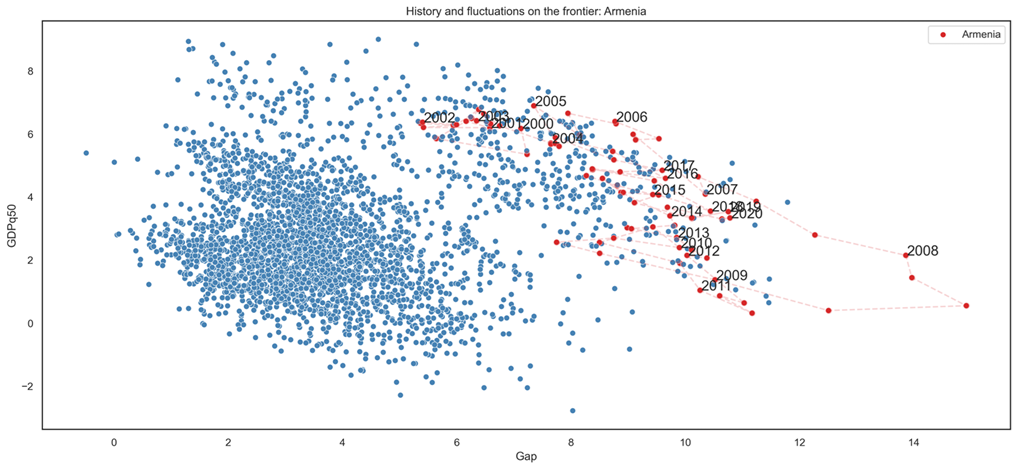
\includegraphics[width=0.9\textwidth, angle=0]{../Figures/arm_position_on_scatter.png}	
	\caption{Armenia's track on the boundary.} 
	\label{fig:arm_position_on_scatter}%
\end{figure}




\subsection{Local model estimation results}
\begin{table}[!ht]
\begin{center}
\caption{In-sample local quantile regression coefficients}
\label{table:local_coeffs}
\scalebox{0.6}{
\begin{tabular}{p{7cm}p{1.5cm}p{1.5cm}p{1.5cm}p{1.5cm}}
\hline
                           & GDP growth, h=4, q=0.1, e=b & GDP growth, h=4, q=0.1, e=f & GDP growth, h=4, q=0.5, e=b & GDP growth, h=4, q=0.5, e=f  \\
\hline
autoregressive             & -0.49***                    & -0.10                       & -0.41***                    & -0.19*                       \\
                           & (0.15)                      & (0.20)                      & (0.09)                      & (0.11)                       \\
const                      & -11.06**                    & 10.90                       & -1.03                       & 5.20*                        \\
                           & (4.60)                      & (7.75)                      & (3.11)                      & (2.95)                       \\
Financial Cycle Index      & 46.43**                     & -63.60*                     & 33.46**                     & -2.61                        \\
                           & (17.72)                     & (31.94)                     & (13.36)                     & (13.15)                      \\
Financial Conditions Index & -2.47                       & 4.83**                      & -2.16                       & 2.34*                        \\
                           & (1.92)                      & (2.02)                      & (1.33)                      & (1.32)                       \\
Liquidity excess           & 56.85**                     & -7.73                       & 28.59**                     & 19.38                        \\
                           & (22.58)                     & (31.87)                     & (13.36)                     & (12.43)                      \\
CAR excess\_C\_2y          & -61.56**                    & -44.55*                     & -23.07                      & -18.15                       \\
                           & (30.67)                     & (25.40)                     & (23.01)                     & (21.13)                      \\
MPI                        & -1.11**                     & 0.14                        & -0.49                       & -0.42                        \\
                           & (0.50)                      & (0.57)                      & (0.37)                      & (0.34)                       \\
FCI x FCyI                 & -4.05***                    & 7.65***                     & -1.50                       & 1.89**                       \\
                           & (1.51)                      & (1.86)                      & (0.96)                      & (0.94)                       \\
MPI x FCyI                 & -0.86*                      & 0.01                        & 0.02                        & -1.40***                     \\
                           & (0.50)                      & (0.83)                      & (0.35)                      & (0.34)                       \\
MPI x FCI                  & -1.34                       & -1.34                       & -0.52                       & 0.10                         \\
                           & (0.97)                      & (0.89)                      & (0.53)                      & (0.45)                       \\
Macroeconomic Indicator    & 21.75***                    & 8.46*                       & 19.36***                    & 11.51***                     \\
                           & (4.11)                      & (4.33)                      & (2.88)                      & (3.11)                       \\
N                          & 77.0000                     & 73.0000                     & 77.0000                     & 73.0000                      \\
Pseudo-R2                  & 0.6597                      & 0.5872                      & 0.4997                      & 0.4726                       \\
\hline \\
\multicolumn{3}{l}{* p<0.05,  ** p<0.01,  *** p<0.001}
\end{tabular}
}
\end{center}
\end{table}
\begin{figure}[!ht]
	\centering 
	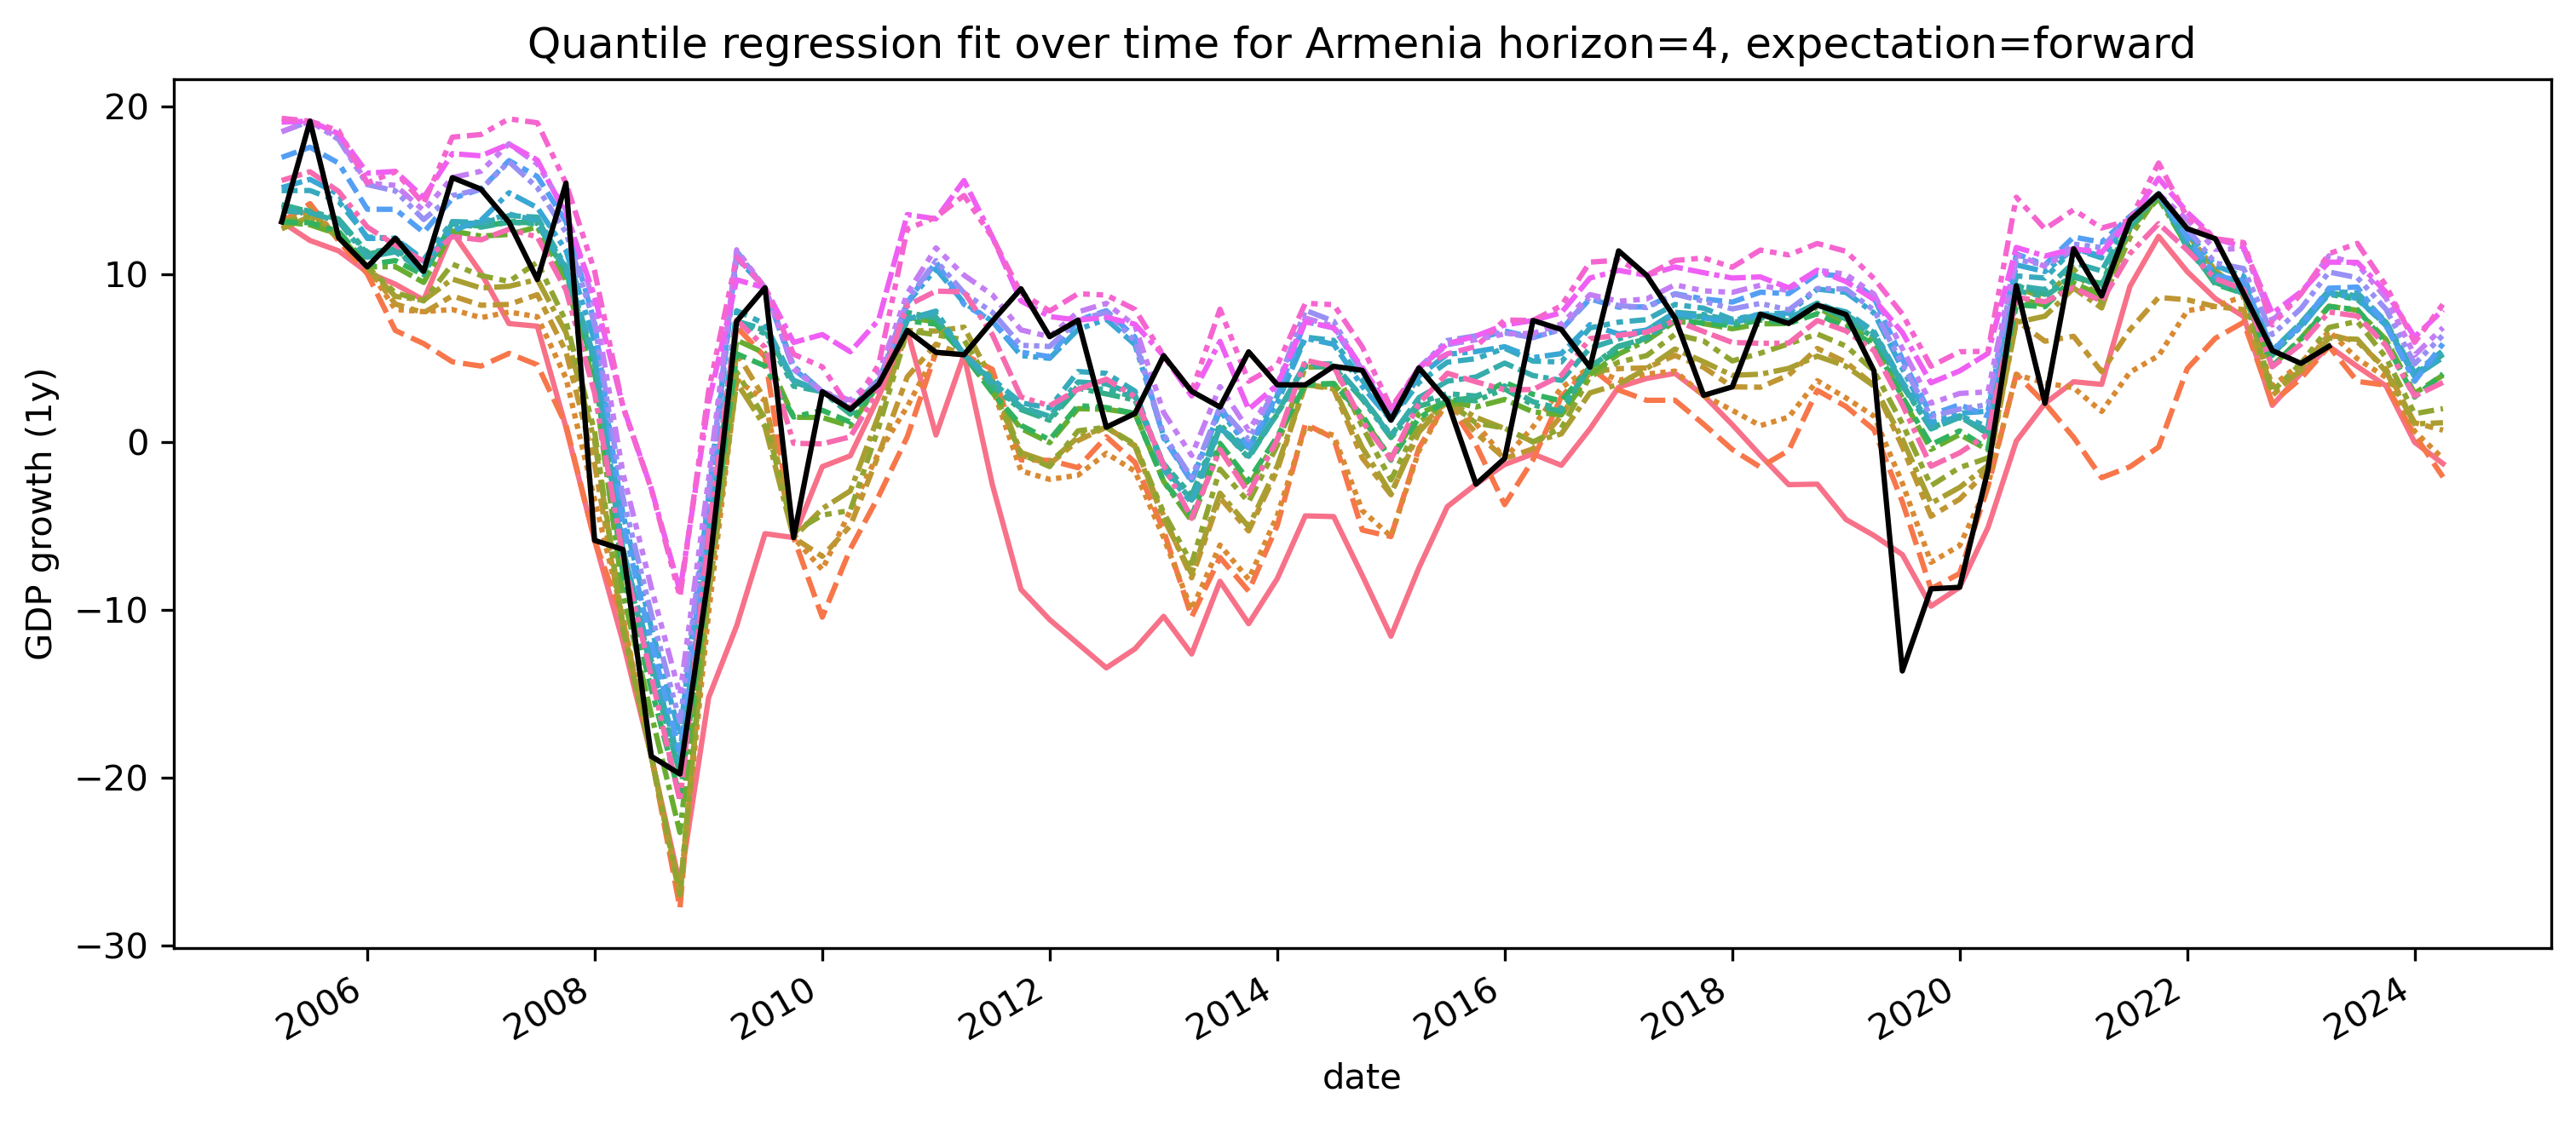
\includegraphics[width=0.9\textwidth, angle=0]{../Figures/arm_qr_f_fits.png}	
	\caption{Local quantile regression one year ahead fitted values of Armenia for different quantiles.} 
	\label{fig:arm_qr_f_fits}%
\end{figure}

\autoref{fig:arm_qr_gdp_kde_dist} shows the GDP growth distribution of Armenia conditional on systemic risks in 2024Q1. Instead of using skewed t-distribution as in \autoref{fig:arm_qr_gdp_dist}, a Kernel density-based estimation is used to interpolate the quantiles. Even though it is more sensitive to the choice of the number of quantiles, it does a better job of describing the left tail of the distribution.
\begin{figure}[!ht]
	\centering 
	
\includegraphics[width=0.9\textwidth, angle=0]{../Figures/arm_qr_gdp_kde_dist.png}	
	\caption{Conditional GDP growth distribution using non-parametric KDE-based interpolation.} 
	\label{fig:arm_qr_gdp_kde_dist}%
\end{figure}



\section{Additional Figures}

\renewcommand{\thefigure}{\thesection.\arabic{figure}}
\setcounter{figure}{0}

\renewcommand{\thetable}{\thesection.\arabic{table}}
\setcounter{table}{0}

\label{appx:additional_figures}
\begin{figure*}[!ht]
	\centering 
	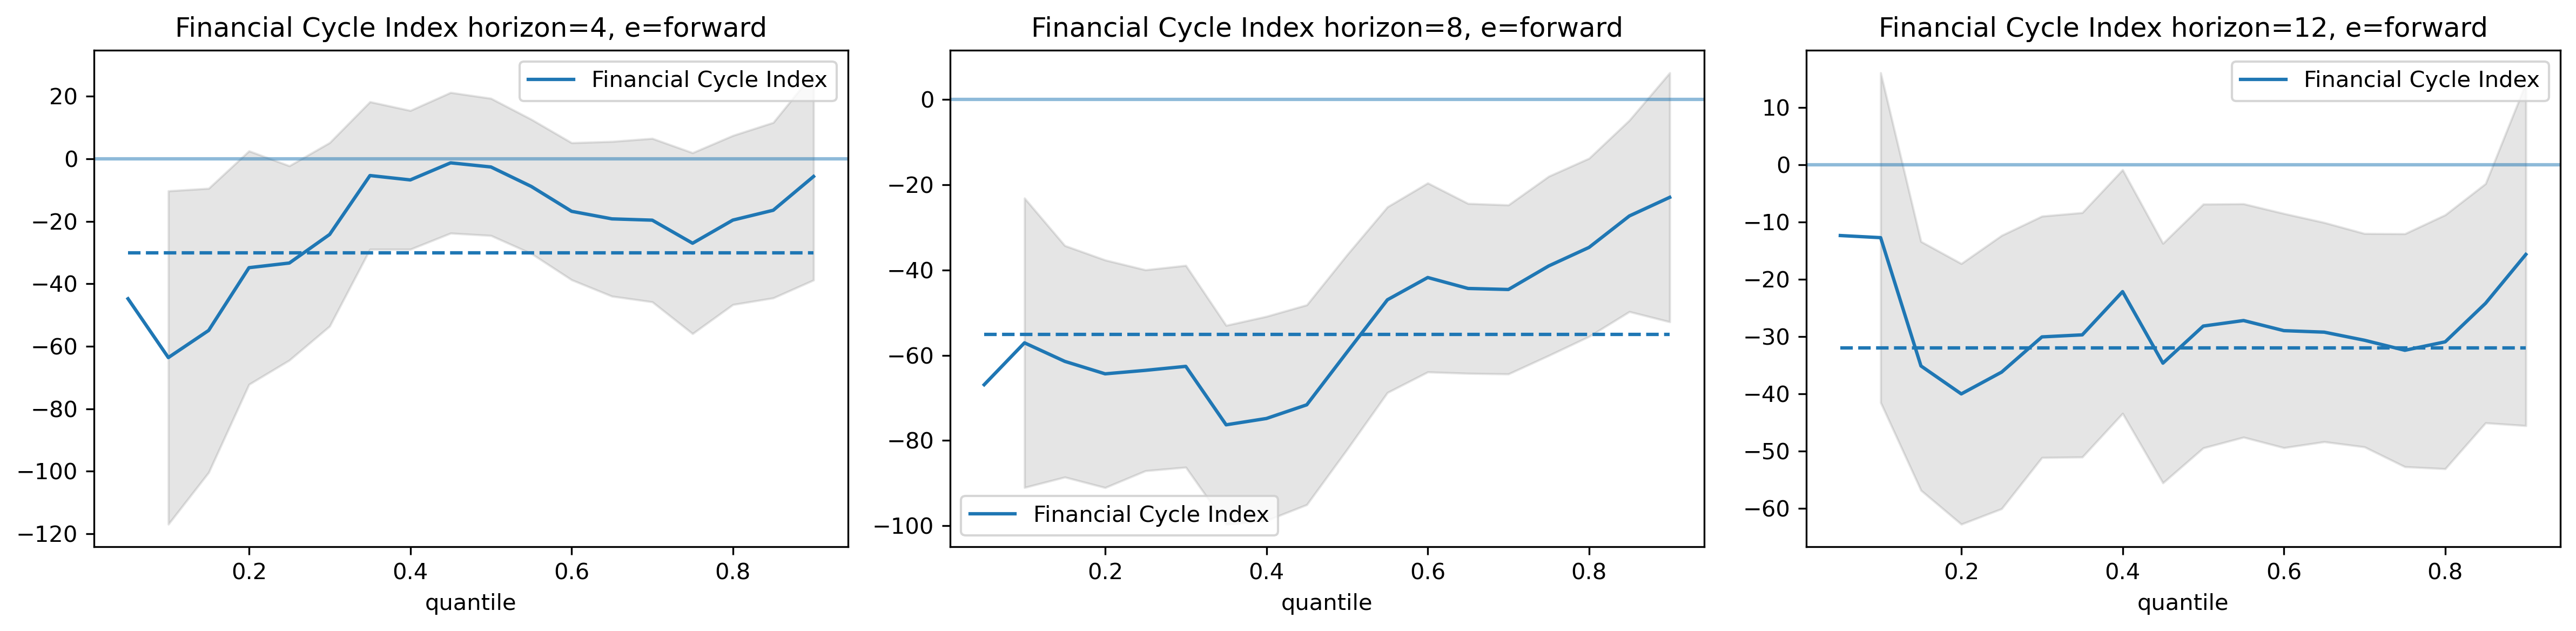
\includegraphics[width=1\textwidth, angle=0]{../Figures/arm_FCyI_f_coeff_quantiles.png}	
	\caption{Local model Financial Cycle Index coefficients. Estimated quantile regression coefficients for horizons 4, 8, and 12. The grey-shaded areas represent the 95\% confidence intervals. The dashed horizontal line presents the OLS coefficient.}
	\label{fig:arm_FCyI_f_coeff_quantiles}%
\end{figure*}
\begin{figure*}[!ht]
	\centering
	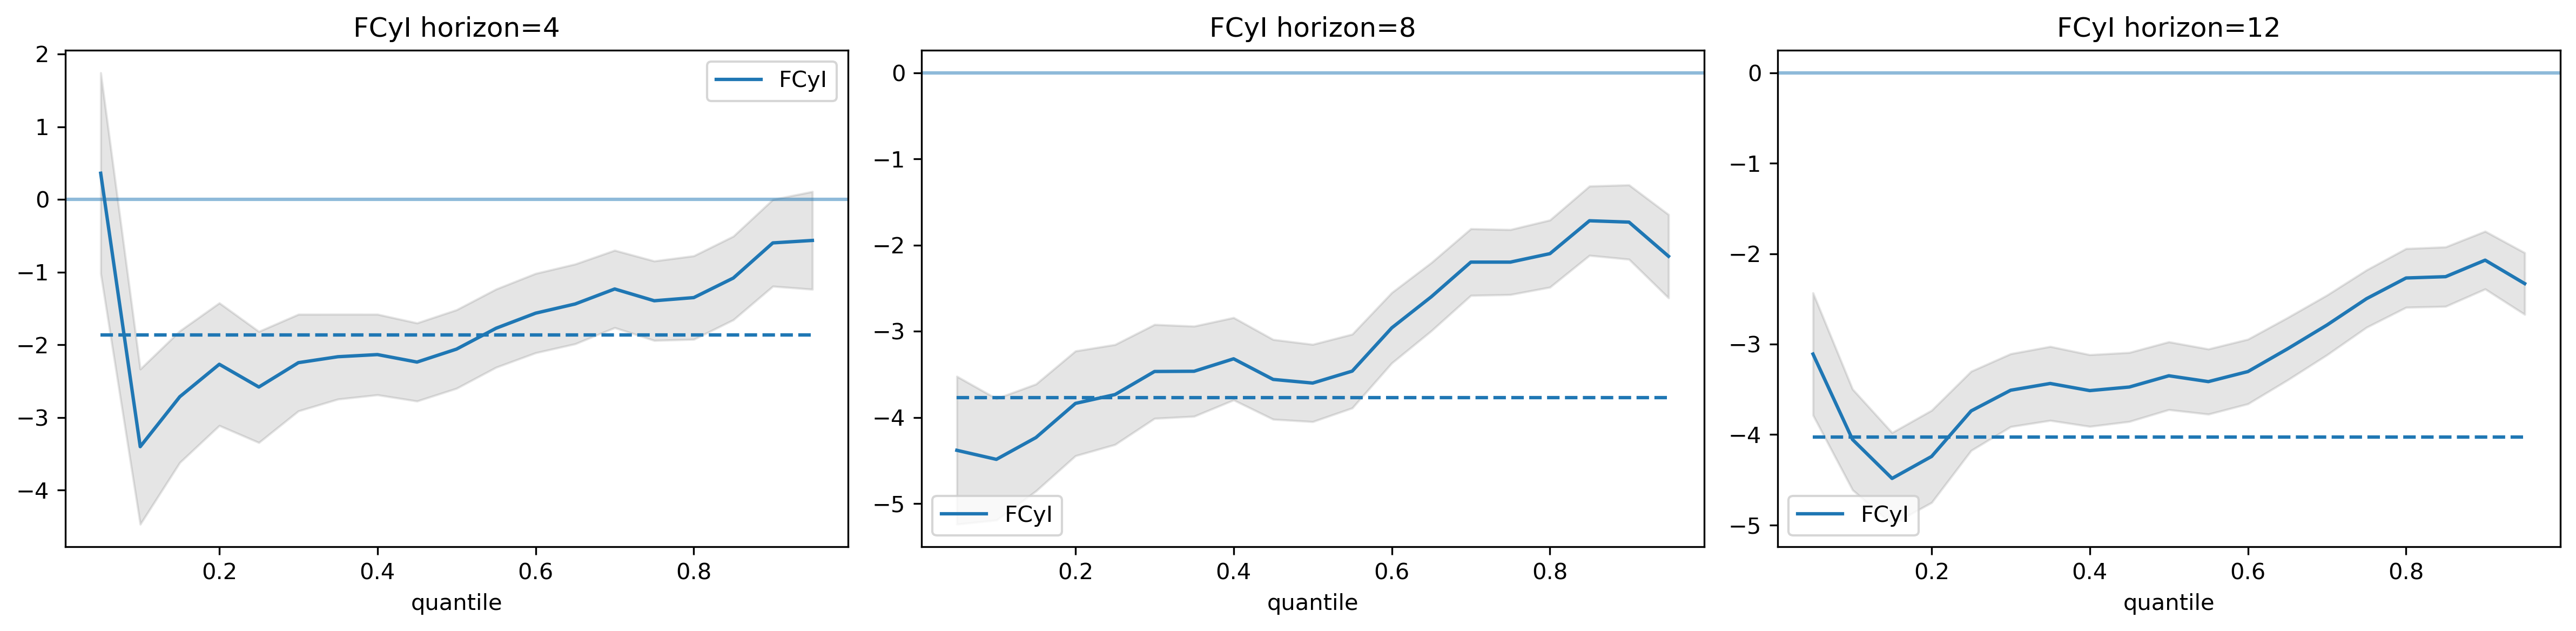
\includegraphics[width=1\textwidth, angle=0]{../Figures/panel_FCyI_coeff_quantiles.png}	
	\caption{Panel model Financial Cycle Index coefficients.} 
	\label{fig:panel_FCyI_coeff_quantiles}%
\end{figure*}
\begin{figure*}[!ht]
	\centering
	
\includegraphics[width=1\textwidth, angle=0]{../Figures/arm_qr_gdp_dist.png}	
	\caption{Conditional GDP growth distribution of Armenia using skewed t-distribution fit for interpolation.}
	\label{fig:arm_qr_gdp_dist}%
\end{figure*}
\begin{figure*}[!ht]
	\centering 
	
\includegraphics[width=1\textwidth, angle=0]{../Figures/arm_FCI_f_coeff_quantiles.png}	
	\caption{Local model Financial Conditions Index coefficients. Estimated quantile regression coefficients for horizons 4, 8, and 12. The grey-shaded areas represent the 95\% confidence intervals. The dashed horizontal line presents the OLS coefficient.}
	\label{fig:arm_FCI_f_coeff_quantiles}%
\end{figure*}
\begin{figure*}[!ht]
	\centering
	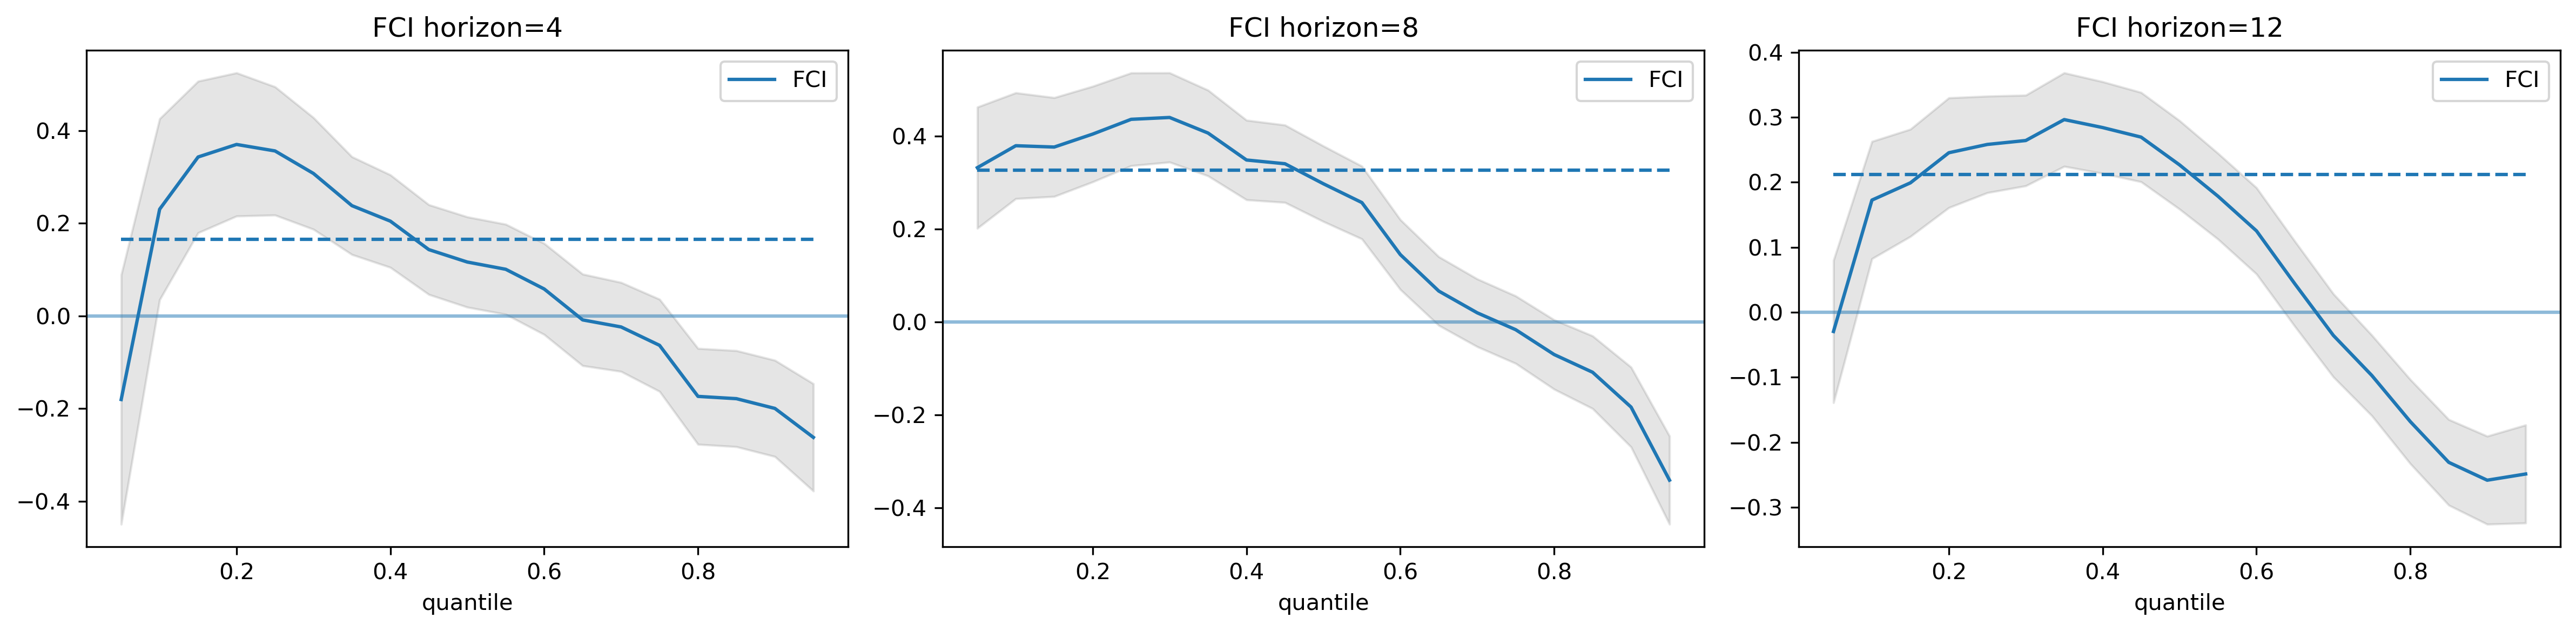
\includegraphics[width=1\textwidth, angle=0]{../Figures/panel_FCI_coeff_quantiles.png}	
	\caption{Panel model Financial Conditions Index coefficients.} 
	\label{fig:panel_FCI_coeff_quantiles}%
\end{figure*}
% \begin{figure*}
% 	\centering
% 	
\includegraphics[width=1\textwidth, angle=0]{Figures/arm_dist_decomp_diff_2024Q1.png}
% 	\caption{Changes in systemic risks between 2023Q1 and 2024Q1 and their impact on the GDP growth.}
% 	\label{fig:arm_dist_decomp_diff_2024Q1}%
% \end{figure*}
% \begin{figure*}[!ht]
% 	\centering
% 	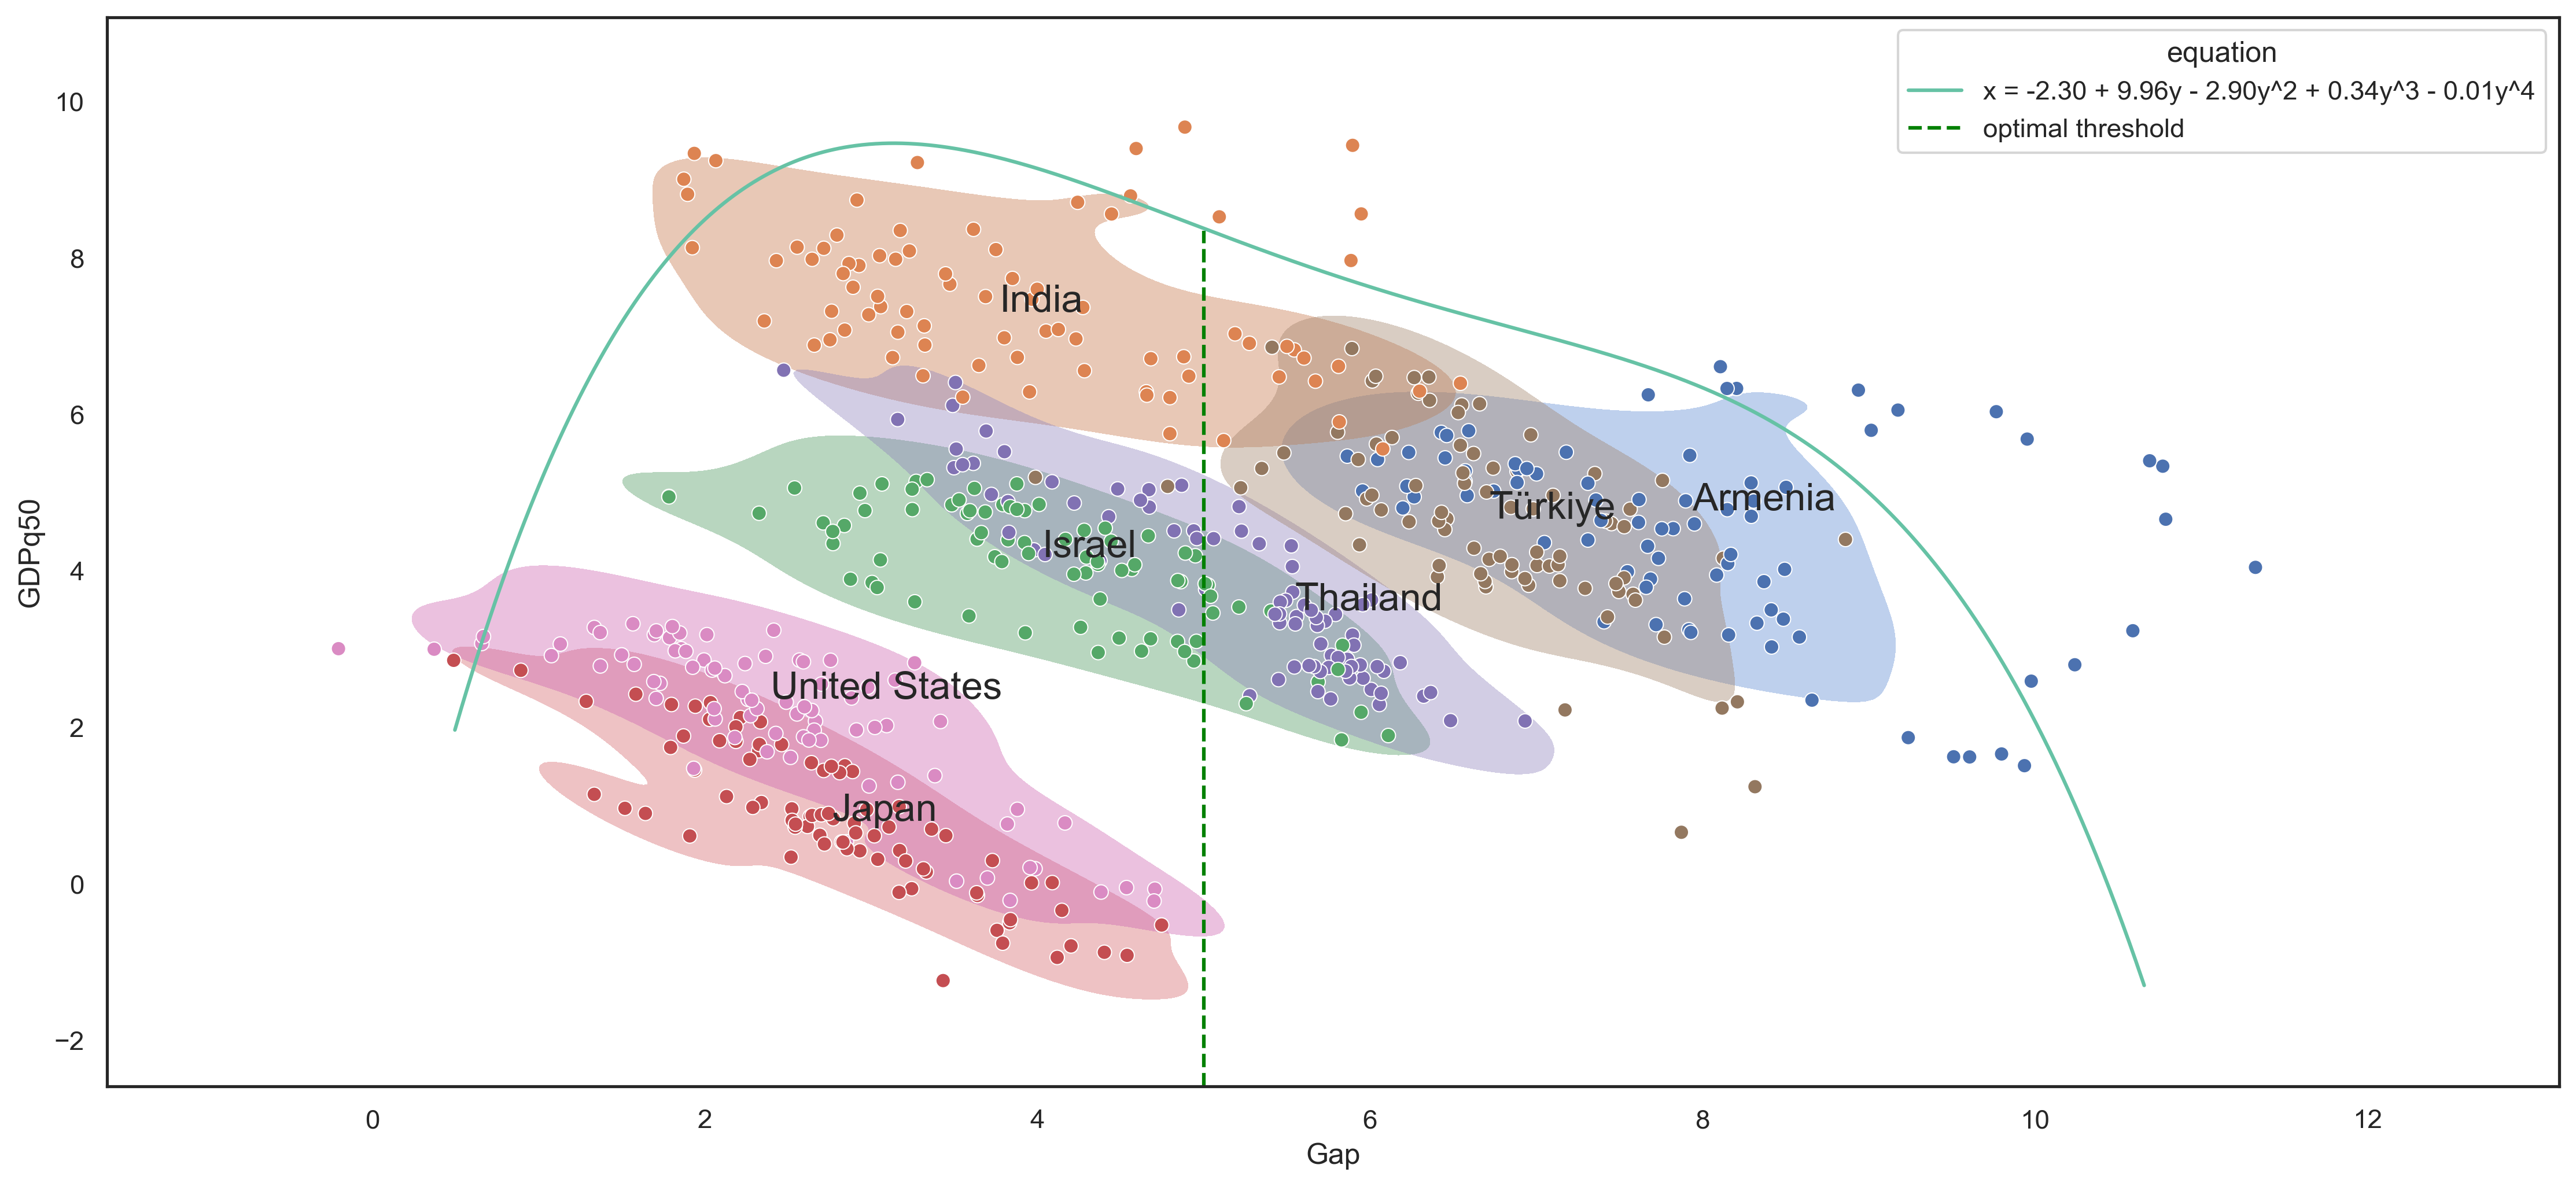
\includegraphics[width=1\textwidth, angle=0]{../Figures/country_cases_that_shape_the_boundary.png}	
% 	\caption{Efficient frontier based on the median and distance-to-tail (Gap) estimates from the 41 countries. The green line represents the frontier and was estimated using a Local Outlier Factor (LOF) algorithm.}
% 	\label{fig:country_cases_that_shape_the_boundary}%
% \end{figure*}
% \begin{figure}[!ht]
% 	\centering 
% 	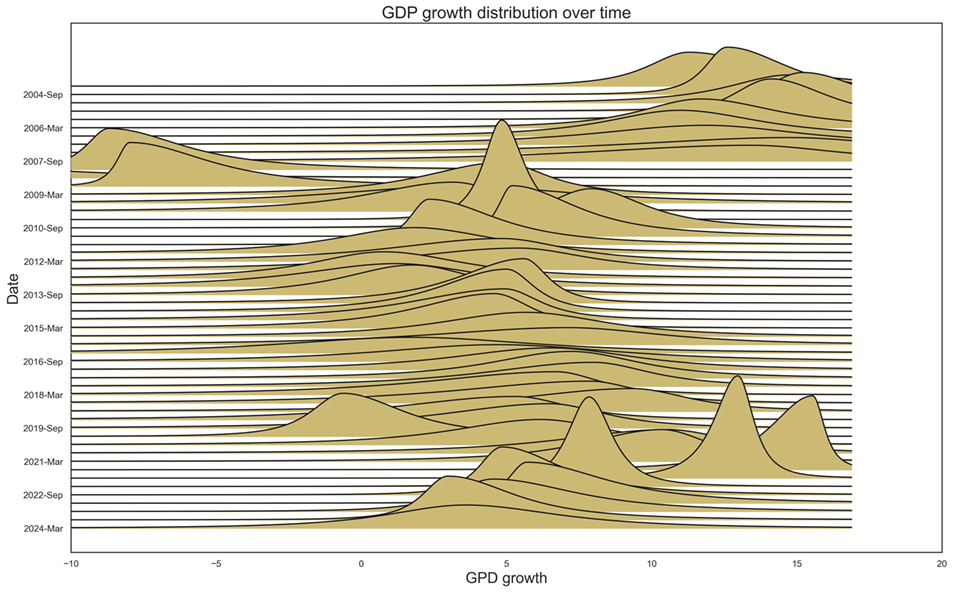
\includegraphics[width=0.9\textwidth, angle=0]{../Figures/arm_ridge_history.png}	
% 	\caption{Fitted historical GDP distributions for Armenia} 
% 	\label{fig:arm_ridge_history}%
% \end{figure}




\end{document}